\documentclass{tudelft-report}
\usepackage{natbib}
\setcitestyle{authoryear, open={[} ,close={]}}				% [Author, Year]
\usepackage{changes}
\usepackage{graphicx}
\usepackage{xcolor,colortbl}
\usepackage{caption}
\usepackage{subcaption}
\usepackage{epstopdf}
\usepackage{float}
\usepackage{enumerate}
\usepackage{wrapfig}
\usepackage{adjustbox}
\usepackage{lscape}
\usepackage{graphicx,wrapfig,lipsum}
\usepackage{multirow}
\usepackage{bm}
\usepackage{amsmath}
\usepackage{siunitx}
\usepackage{comment}

\sisetup{detect-all}

%%Nomenclature
\usepackage{nomencl}
\makenomenclature
\usepackage{etoolbox}
\renewcommand\nomgroup[1]{%
\item[\bfseries
 \ifstrequal{#1}{A}{Roman Symbols}{%
  \ifstrequal{#1}{G}{Greek Symbols}{%
  \ifstrequal{#1}{Z}{Abbreviations}{}}}%
]}
\newcommand{\nomunit}[1]{%
\renewcommand{\nomentryend}{\hspace*{\fill}#1}}




\begin{document}

%% Use Roman numerals for the page numbers of the title pages and table of
%% contents.
\frontmatter

\title{Decreasing the surface turbidity due to overflow losses on a TSHD - A preliminary study}
\author{F.B.\ Tims}
\affiliation{Technische Universiteit Delft}
\coverimage{Images/Dredge.jpg}
\makecover

%% Include an optional title page.
\begin{titlepage}

\begin{center}

%% Insert the TU Delft logo at the bottom of the page.
\begin{tikzpicture}[remember picture,overlay]
    \node at (current page.south)[anchor=south,inner sep=0pt]{
        
\includegraphics{cover/logo}
        
\includegraphics[scale=0.55]{Images/APT.jpg}
    };
\end{tikzpicture}

%% Extra whitespace at the top.
\vspace*{2\bigskipamount}

%% Print the title in cyan.
{\makeatletter
\titlestyle\color{tudelft-cyan}\Huge \@title 
\makeatother}

%% Print the optional subtitle in black.
{\makeatletter
\ifx\@subtitle\undefined\else
    \bigskip
    \titlefont\titleshape\LARGE\@subtitle
\fi
\makeatother}

\bigskip
\bigskip

by
%door

\bigskip
\bigskip

%% Print the name of the author.
{\makeatletter
\titlefont\Large\bfseries\@author
\makeatother}

\vfill

in partial fulfillment of the requirements for the degree of
%in overeenstemming met de vereisten voor het verkrijgen van de graad van

\bigskip
\bigskip

{\bfseries Master of Science}

in Applied Physics

\bigskip
\bigskip

at the Delft University of Technology,
%aan de Technische Universiteit Delft,

to be defended publicly on Tuesday January 1, 2013 at 10:00 AM.
%in het openbaar de verdedigen op dinsdag 1 januari om 10:00 uur.

\vfill

\begin{tabular}{lll}
%% Add additional information here, per faculty requirements, e.g
   Student number: & 4418808 \\
    Project duration: & \multicolumn{2}{l}{February 19, 2018 -- \today} \\
    Chairman: & Dr.\ Ir. \ G.H. \ Keetels, & TU Delft \\
    Thesis committee:
        & Prof.\ dr.\ ir. \ C.\ van Rhee, & TU Delft \\
        & Ir.\ G.\ Teheux, & APT Offshore BV \\
        & Dr.\ E.\ L.\ Brown, & TU Delft \\
    External: & Ir. \ U. \ Andersen, & Rohde Nielsen
        
\end{tabular}

%% Only include the following lines if confidentiality is applicable.
\bigskip
\bigskip
\emph{This thesis is confidential and cannot be made public until December 31, 2019.}
%\emph{Op dit verslag is geheimhouding van toepassing tot en met 31 december 2013.}

\bigskip
\bigskip
An electronic version of this thesis is available at \url{http://repository.tudelft.nl/}.
%Een elektronische versie van dit verslag is beschikbaar op \url{http://repository.tudelft.nl/}.

\end{center}

\end{titlepage}



\chapter*{Preface}
\setheader{Preface}

Preface\ldots

%Thanks to APT en Rohde Nielsen (+ Persons), TU Delft staff, family etc.
%Frans van Grunsven & Wesley Pont, Ed Stok en Freek Brakel



\begin{figure}
    \centering
    \begin{subfigure}[b]{0.6\textwidth}
        
\includegraphics[scale=0.5]{Images/APT.jpg}
    \end{subfigure}
    ~ %add desired spacing between images, e. g. ~, \quad, \qquad, \hfill etc. 
      %(or a blank line to force the subfigure onto a new line)
    \begin{subfigure}[b]{0.22\textwidth}
        
\includegraphics[scale=0.1]{Images/RD.jpg}
       
    \end{subfigure}
\end{figure}

\begin{flushright}
{\makeatletter\itshape
    \@author \\
    Delft, \today
\makeatother}
\end{flushright}


\chapter*{Summary}
\addcontentsline{toc}{chapter}{Summary}
\chapter*{Samenvatting}
\addcontentsline{toc}{chapter}{Samenvatting}

\tableofcontents
\listoffigures
\listoftables
%\chapter*{Nomenclature}
\addcontentsline{toc}{chapter}{Nomenclature}

\makenomenclature

\printnomenclature

\printnomenclature


%% Use Arabic numerals for the page numbers of the chapters.
\mainmatter


\chapter{Introduction}

\section{Overview TSHD}
%\textbf{Omschrijving schip werkwijze + kort vulling hopper}
%\textbf{Van Rhee PhD + lecturenotes Dredging processes}

The Trailing suctions hopper dredger (TSHD) is a ship that is equipped with one or two suction pipes, which are lowered to the seabed during dredging operations. A water-sediment mixture is sucked up to the ship which will be discharged in the cargo hold, also called the hopper of the ship. The hopper is filled, where the sand particles settle and excess water flows overboard. The loading process of a TSHD is shown in figure \ref{fig:loading}\citep{Lecture}.\newline

\begin{figure}[ht!]
    \centering
    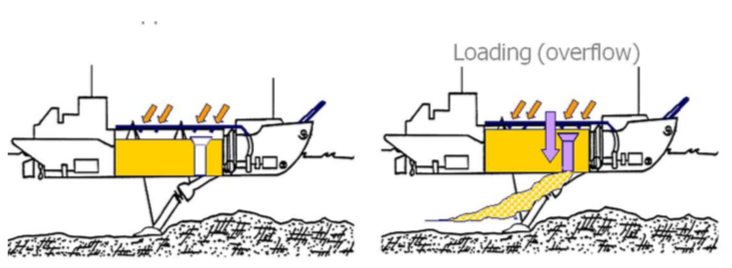
\includegraphics[width=0.8\linewidth]{Images/TSHD_loading.png}
    \caption{Loading process of a TSHD}
    \label{fig:loading}
\end{figure}
\noindent
After the loading process, the TSHD sails to the designated location where the hopper is discharged by opening the doors in the bottom of the ship, pumping the sediment ashore or by rain bowing, which is shown in figure \ref{fig:Rainbow}

\begin{figure}[ht!]
    \centering
    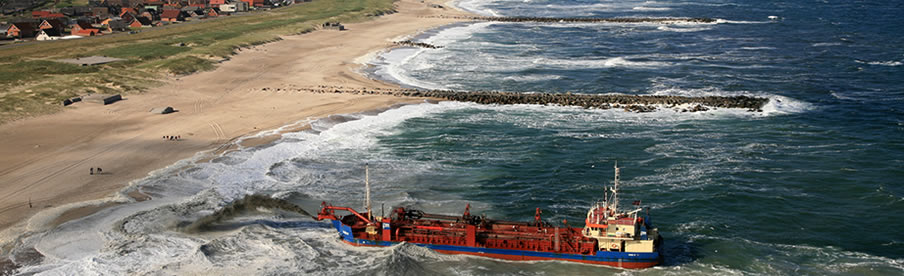
\includegraphics[width=0.8\linewidth]{Images/Rainbow.jpg}
    \caption{Discharge of TSHD by rain bowing}
    \label{fig:Rainbow}
\end{figure}

\noindent
The hopper inlet system varies between ships, but the general aim is to divide the water-sediment mixture over the width of the hopper. During the loading process, the hopper is filled with water to obtain a water level inside the hopper equal to outside. The inlet loading pipes discharge the sucked up water-sediment mixture inside the hopper. The sand particles settle and will form a bed, which grows during the loading process. 




%%%%%%%%%%%%%%%%%%%%%%%%%%%%%%%%%%%%%%%%%%%%%%%%%%%%%%%%%%%%%%%%%%%%%%%%%%%%%%%%%%%%%%%%%%%%%%%%%%%%%%%%%%%%%%%%%%%%%%%%%%%%%%%%%%%%%%%%%%%%%%%%%%%%%%%%%%%%


\section{Description of overflow}

%\textbf{Types of overflow} \newline
%\textbf{Info bij van Rhee winnen} \newline
%\textbf{Tekening overflow (bijlage)}

The excess water flows overboard through the overflow. The commonly used overflows these days are adjustable in the vertical to regulate the overflow in the hopper. An overview of an overflow is shown in figure \ref{fig:Overflow}. 

\begin{figure}[ht!]
    \centering
    \includegraphics[width=0.8\linewidth]{Images/}
    \caption{Cross section of hopper with overflow}
    \label{fig:Overflow}
\end{figure}

\noindent
The overflow will transport the excess water underneath the hull into the surrounding water. However, not every sand particle will settle inside the hopper due to the current from the inlets to the overflow inside the hopper. With the dividing of the water-sediment mixture over the hopper dimension the process is more or less controlled to load as fast as possible, and so, to lose as less sand particles through the overflow. Despite this, the control of the process is very hard and so sand particles are lost through the overflow.\newline

%Werking Overflow vragen Vrhee / Rhode Nielsen




%%%%%%%%%%%%%%%%%%%%%%%%%%%%%%%%%%%%%%%%%%%%%%%%%%%%%%%%%%%%%%%%%%%%%%%%%%%%%%%%%%%%%%%%%%%%%%%%%%%%%%%%%%%%%%%%%%%%%%%%%%%%%%%%%%%%%%%%%%%%%%%%%%%%%%%%%%%%


\section{Ecological effects of sediment turbidity}
The dredging process with a TSHD may lead to increased turbidity, higher suspended concentrations and enhanced sediment deposition. This mainly affects performance of visual predators and growth and survival of bottom vegetation as is shown in figure \ref{fig:Ecoligical}. However it is not understood yet, how large this impact is and whether it results in real problems. The circumstances in the sea and on and in the bed may change, but it is not clear if and how it will affect the flora and fauna in this region. The tolerance levels of different species of plant and animals differ from each other. Therefore some species may profit from increased sedimentation or suspended matter concentrations, whilst others do not survive a slight change in living environment. An important aspect is the kind of material that is released into the water. Clay particles together with organic material can form large coagulates that absorb a lot of light, while the organic material is also a source of food. In contrast a same weight of sand particles absorbs almost no light. \citep{Dankers} \newline
Turbidity at a certain distance from the ship can be reduced, however, turbidity around the ships location can not disappear. Therefore the ecological effect of turbidity is more important for passive plumes that travel far field.

\begin{figure}[ht!]
    \centering
    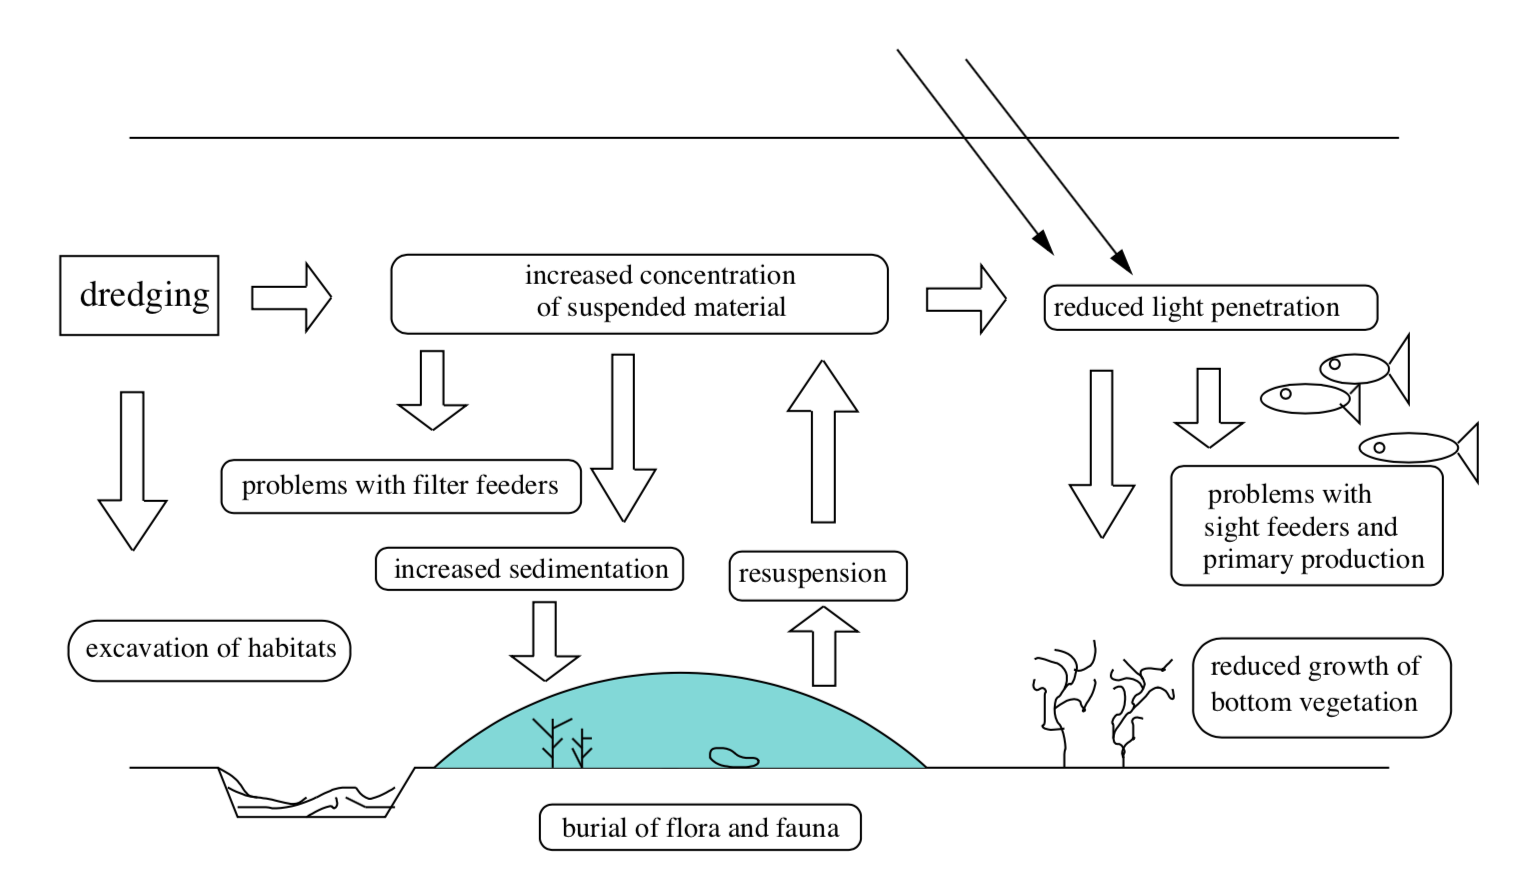
\includegraphics[width=.75\linewidth]{Images/Ecological.png}
    \caption{Ecological effect dredging}
    \label{fig:Ecoligical}
\end{figure}

%%%%%%%%%%%%%%%%%%%%%%%%%%%%%%%%%%%%%%%%%%%%%%%%%%%%%%%%%%%%%%%%%%%%%%%%%%%%%%%%%%%%%%%%%%%%%%%%%%%%%%%%%%%%%%%%%%%%%%%%%%%%%%%%%%%%%%%%%%%%%%%%%%%%%%%%%%%%

\section{Research Aim}

The aim of this master thesis is to provide insight in which factors influence the amount of surface turbidity and provide a practical solution to decrease the surface turbidity. The turbidity has ecological ans visual impact and should be decreased for ecological regulations.

%%%%%%%%%%%%%%%%%%%%%%%%%%%%%%%%%%%%%%%%%%%%%%%%%%%%%%%%%%%%%%%%%%%%%%%%%%%%%%%%%%%%%%%%%%%%%%%%%%%%%%%%%%%%%%%%%%%%%%%%%%%%%%%%%%%%%%%%%%%%%%%%%%%%%%%%%%%%

\section{Research Methodology}

\noindent The research methodology is characterized by the following steps:
\begin{itemize}
    \item Description dredging processes in the near field
    \item Find out which factors influence the creating of a surface plume
    \item Experiments (Practical)
    %\item Practical solution
\end{itemize}  






%%%%%%%%%%%%%%%%%%%%%%%%%%%%%%%%%%%%%%%%%%%%%%%%%%%%%%%%%%%%%%%%%%%%%%%%%%%%%%%%%%%%%%%%%%%%%%%%%%%%%%%%%%%%%%%%%%%%%%%%%%%%%%%%%%%%%%%%%%%%%%%%%%%%%%%%%%%%

\section{Outline}



%%%%%%%%%%%%%%%%%%%%%%%%%%%%%%%%%%%%%%%%%%%%%%%%%%%%%%%%%%%%%%%%%%%%%%%%%%%%%%%%%%%%%%%%%%%%%%%%%%%%%%%%%%%%%%%%%%%%%%%%%%%%%%%%%%%%%%%%%%%%%%%%%%%%%%%%%%%%

%NOMENCLATURE

\nomenclature[Z]{TSHD}{Trailing Suction Hopper Dredger}
\nomenclature[A]{$g$}{Gravity acceleration \nomunit{[$m/s^2$]}}


\chapter{Description Dredging Processes}

INTRO met verwijzingen


\newpage
\section{Sedimentation in hopper \& overflow losses}
\label{sec:hopper}

Research on the sedimentation process is carried out by multiple professors like \citep{Miedema_Vlasblom}, \citep{Ooijens} and \citep{Rhee}. All their models are based on the \citep{Camp} model, a settling basin theory model which was developed for waste water treatment. The Camp model is a strongly simplified flow field where no vertical flow and constant flow depth are assumed. The description of the Camp model is shown in figure \ref{fig:Camp}. It can be seen that all particles having a settling velocity larger than v$_0$ enter the sludge zone and therefore are removed from the flow. Particles having a smaller settling velocity w$_s$ only enter the sludge zone when they enter the settling zone between point b and c.

\begin{figure}[ht!]
    \centering
    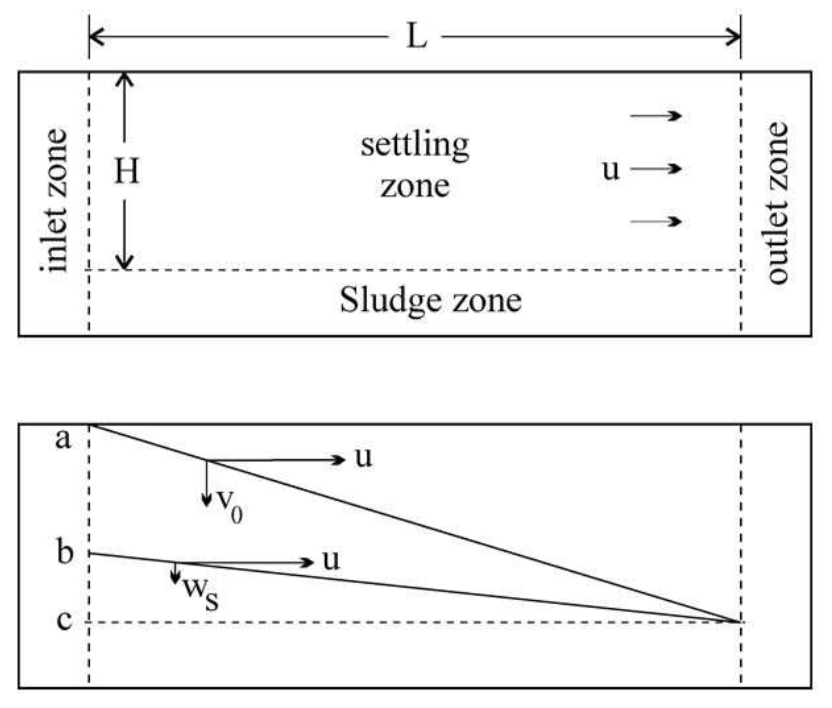
\includegraphics[width=.6\linewidth]{Images/Camp.png}
    \caption{Ideal settling basin according to Camp}
    \label{fig:Camp}
\end{figure}

\noindent \cite{Miedema_Vlasblom} used the Camp model as the basis for their model, but added sorting, erosion, the hindered settling effect and the influence of a rising sand bed. In addition, \cite{Ooijens} added dynamics for example the time effect, which was added by regarding the hopper as an ideal mixing tank. \cite{Miedema_Vlasblom} assumed an equal inflow concentration and concentration in the hopper and a instantaneous reaction of the outflow concentration on the determined settling efficiency. \cite{Ooijens} used the calculated concentration in the hopper for the settling efficiency. \\
\noindent An important quantity during the loading process is the overflow loss. Two different definitions are known. The loss can be defined as the ratio of the total outflow and inflow volume or as the ratio of the outflow and inflow sand flux at a certain moment \citep{Rhee}.\newline \newline
The overflow flux is defined as:

\begin{equation}
\label{eq:OV_flux}
    OV_{flux}(t) = \frac{Q_o(t) C_o(t)}{Q_i(t) C_i(t)}
\end{equation}
\nomenclature[A]{$Q_o$}{Outflow discharge \nomunit{[$m^3/s$]}}
\nomenclature[A]{$Q_i$}{Inflow discharge \nomunit{[$m^3/s$]}}
\nomenclature[A]{$C_o$}{Outflow concentration \nomunit{[-]}}
\nomenclature[A]{$C_i$}{Inflow concentration \nomunit{[-]}}
\nomenclature[A]{$OV_{flux}$}{Overflow flux \nomunit{[-]}}
\nomenclature[A]{$OV_{cum}$}{Cumulative overflow flux \nomunit{[-]}}
\nomenclature[Z]{$OV$}{Overflow Loss}


\noindent The cumulative overflow loss is defined as:

\begin{equation}
\label{eq:OV_cum}
    OV_{cum}(t) = \frac{\int_{0}^{t} Q_o(t) C_o(t) dt}{\int_{0}^{t} Q_i(t) C_i(t) dt}
\end{equation}
\newline
\noindent \textit{Q} is the discharge and \textit{C} the volume concentration. The indices \textit{i} and \textit{o} are related to the inflow and outflow in the hopper \citep{Rhee}. When the sedimentation processes in the hopper are taken into account, the overflow losses can be described as a function of the concentration in the hopper \textit{$C_v$}, the average flow \textit{$Q_{ave}$}, the height of the bed in the hopper \textit{$h_s$}, grain size \textit{$D_{50}$} and the grain size uniformity \textit{$cu$} which is the \textit{$D_{60}$/$D_{10}$} ratio \citep{Ooijens}. Therefore, the overflow loss can be described as:

\begin{equation}
\label{eq:OV}
    OV = f(C_v, Q_{ave}, h_s, D_{50}, cu)
\end{equation} \newline

\noindent However, \cite{Ooijens} assumed a steady state in his model and therefore processes like erosion, local flow and concentration are neglected. \cite{Ooijens} and others distinguished four stages of overflow loss in time as shown in figure \ref{fig:phases_overflow_loss}.

\begin{figure}[ht!]
    \centering
    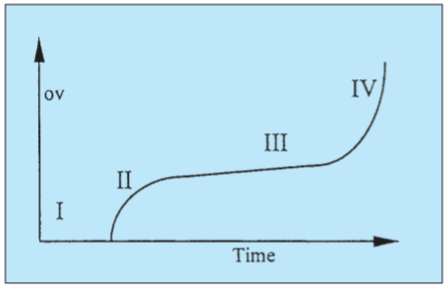
\includegraphics[width=.5\linewidth]{Images/Phases_overflow_loss.png}
    \caption{Stages of overflow losses}
    \label{fig:phases_overflow_loss}
\end{figure}

\begin{enumerate}[I]
    \item Before the overflow level is reached there is no outgoing flow and so, no overflow losses. In this phase the horizontal velocity in the hopper is low, which means good sedimentation of the sediment. The average concentration of the mixture in the hopper will be relatively low when the overflow is reached. The volume during this phase is constant.
    \item Stage II is a transition stage between I and III. When the overflow level is reached, overflowing starts and therefore the velocity in the hopper will increase. The increasing average velocity causes a decreasing settling efficiency. The average concentration in the hopper slowly increases, causing a decreasing settling velocity and an increasing overflow loss. The volume during this phase will decrease.
    \item A steady-state phase emerges in which only the volume of the mixture and the horizontal velocity will slowly increase. The overflow losses are quite constant in this phase, until the scouring velocity is reached.
    \item The horizontal velocity in the hopper will increase and scouring will dominate the settling process when the free volume in the hopper decreases. This increases the overflow losses strongly and decreases the volume in the hopper.
\end{enumerate}

\noindent This theory with different phases is however outdated by the research of \cite{Rhee} where several experiments are carried out in a rectangular laboratory flume with a glass side wall, where flow patterns could be monitored. \cite{Rhee} concluded that the hopper area can be divided into five different sections (figure \ref{fig:overview_hopper_flowfield}), where A is the inflow and B is the density current.


\begin{figure}[ht!]
    \centering
    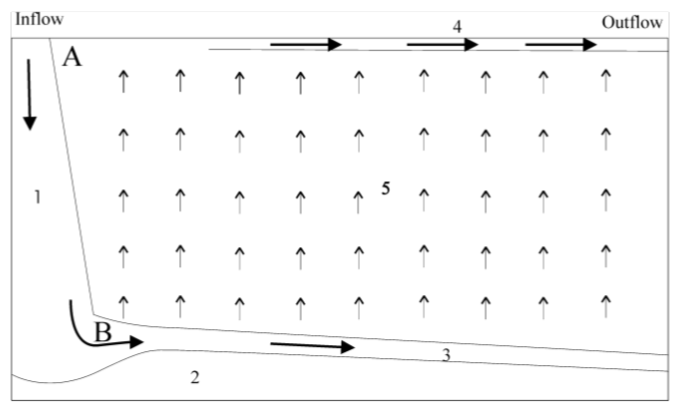
\includegraphics[width=.6\linewidth]{Images/Overview_hopper_flowfield.png}
    \caption{Schematic overview of flow field in hopper.}
    \label{fig:overview_hopper_flowfield}
\end{figure}

\noindent The five different sections are divided in:

\begin{enumerate}
    \item Inflow section
    \item Settled sand / stationary bed
    \item Density flow over settled bed
    \item Horizontal flow at the surface towards overflow
    \item Suspension in remaining area
    
\end{enumerate}

\noindent The incoming mixture (A) flows towards the bottom and forms an erosion crater and density current (B). From this current, sedimentation will take place where coarser particles will settle first which results in a rising bed level. A part of the incoming sediment which does not settle (fine particles) will go up in suspension. When the overflow level is reached, the surface water creates a horizontal current to the overflow. This process is continued until the hopper is completely filled with sediment.\newline \cite{Rhee} measured the the particle size distribution at the inflow and outflow where the overflow samples showed a large variation of particle size distribution, becoming coarser in time. The increasing grain diameter in the overflow is related to the increasing concentration in the overflow. Due to hindered settling, the settling velocity decreases with concentration and therefore larger particles remain in suspension and are removed with the overflow. Also, erosion of the bed at the surface when the hopper is almost totally filled, adds coarser materials to the overflow. \newline
\cite{Rhee} used the observed flow field and grain size distributions to develop a numerical 1DV model to determine the overflow losses. Instead of the Camp model, which uses a horizontal one-dimensional approach with a horizontal supply on one side and overflow on the other. The 1DV model of \cite{Rhee} is a vertical model, where sediment is supplied from the bottom and the overflow is located at the top. In addition, the influence of the hopper load parameter and the mutual interaction of the different grain sizes of the particle size distribution is implemented. The numerical 1DV model was compared with hopper sedimentation tests where a good correlation was shown between the model and the experiments. However, horizontal transport and erosion is not accounted for in the 1DV model and probably scale effects are present. Therefore the model can not be guaranteed to be in agreement with reality. \newline In order to include horizontal transport, \cite{Rhee} extended the 1DV model to a 2DV model. A boundary condition at the interface between the settled sediment and the mixture above had to be formulated for the numerical model. In order to do this, sedimentation tests where done in the laboratory and an empirical relation between the bed shear stress and the reduction of the sedimentation flux was found. This empirical relation was built in the 2DV model, after which the model was validated and found to agree well with laboratory- and prototype measurements.

\nomenclature[Z]{1DV}{One Dimensional}
\nomenclature[Z]{2DV}{Two Dimensional}
%%%%%%%%%%%%%%%%%%%%%%%%%%%%%%%%%%%%%%%%%%%%%%%%%%%%%%%%%%%%%%%%%%%%%%%%%%%%%%%%%%%%%%%%%%%%%%%%%%%%%%%%%%%%%%%%%%%%%%%%%%%%%%%%%%%%%%%%%%%%%%%%%%%%%%%%%%%%%%%%%%%%%%%%%%%%%%

\section{Description of overflow plumes}
\label{sec:plume}
%\textbf{Near-, mid- and far field dredging plume} 

The water-sediment mixture that leaves the overflow may have large ecological impact. This depends on, among other things, how the sediment is distributed when leaving the overflow. Upon release from the bottom of the ship, the water-sediment mixture forms a negative-buoyant plume, which is either mixed directly with the ambient water or behaves as a density current \citep{Winterwerp}. Plumes that are mixed directly are called passive plumes and plumes that behave as a density current are called dynamic plumes. \\\\

\noindent \textbf{Dynamic Plumes} \newline
Dynamic plumes, shown in figure \ref{fig:dynamic_plume} \citep{Dankers}, descend rapidly as a current to the seabed and spread radially across the seabed as a dense plume, slowing down in time and distance as the kinetic energy is lost due to friction. The bulk behaviour of the water-sediment mixture rather than the individual settling velocity is important \citep{Winterwerp}. Because of the rather high (bulk) settling velocity of a dynamic plume, the zone of impact is small.
\begin{figure}[ht!]
    \centering
    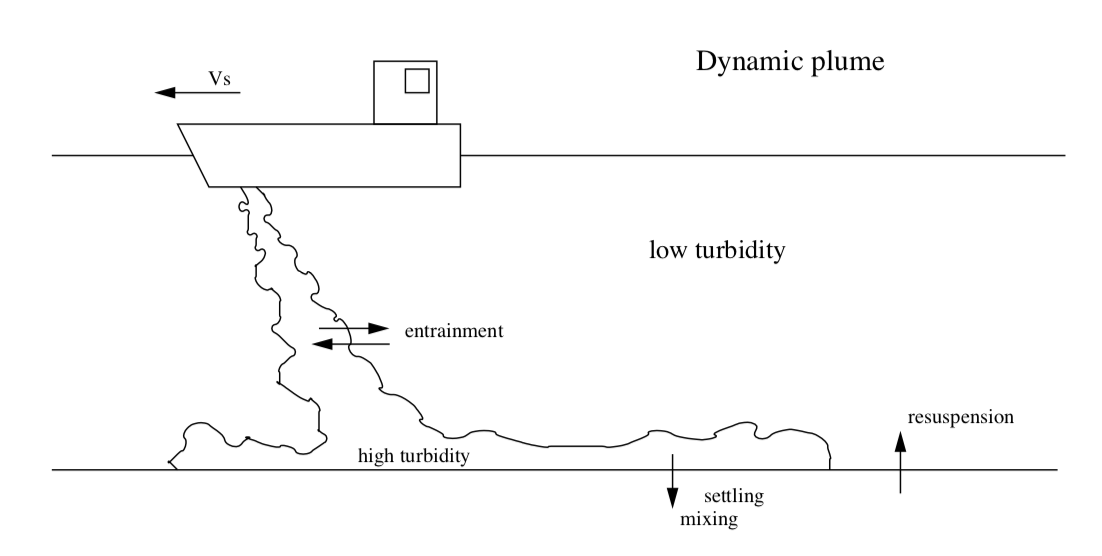
\includegraphics[width=.85\linewidth]{Images/Plume_dynamic.png}
    \caption{Dynamic plume phase }
    \label{fig:dynamic_plume}
\end{figure}

\noindent \textbf{Cloud formation}\newline
A particular case of a dynamic plume develops when the outflow of the overflow is discontinuous. Clouds of sediment, water and air bubbles that entered the overflow due to the discontinuous outflow of the overflow are formed that does not behave as a dynamic plume shown in figure \ref{fig:dynamic_plume}. This phenomena is called cluster settling, convective settling or cloud formation. Clouds can also form from density currents by stretching and eventually 'breaking' in different parts. The cloud formation is presented in figure \ref{fig:cloud_plume} \citep{Dankers}.

\begin{figure}[ht!]
    \centering
    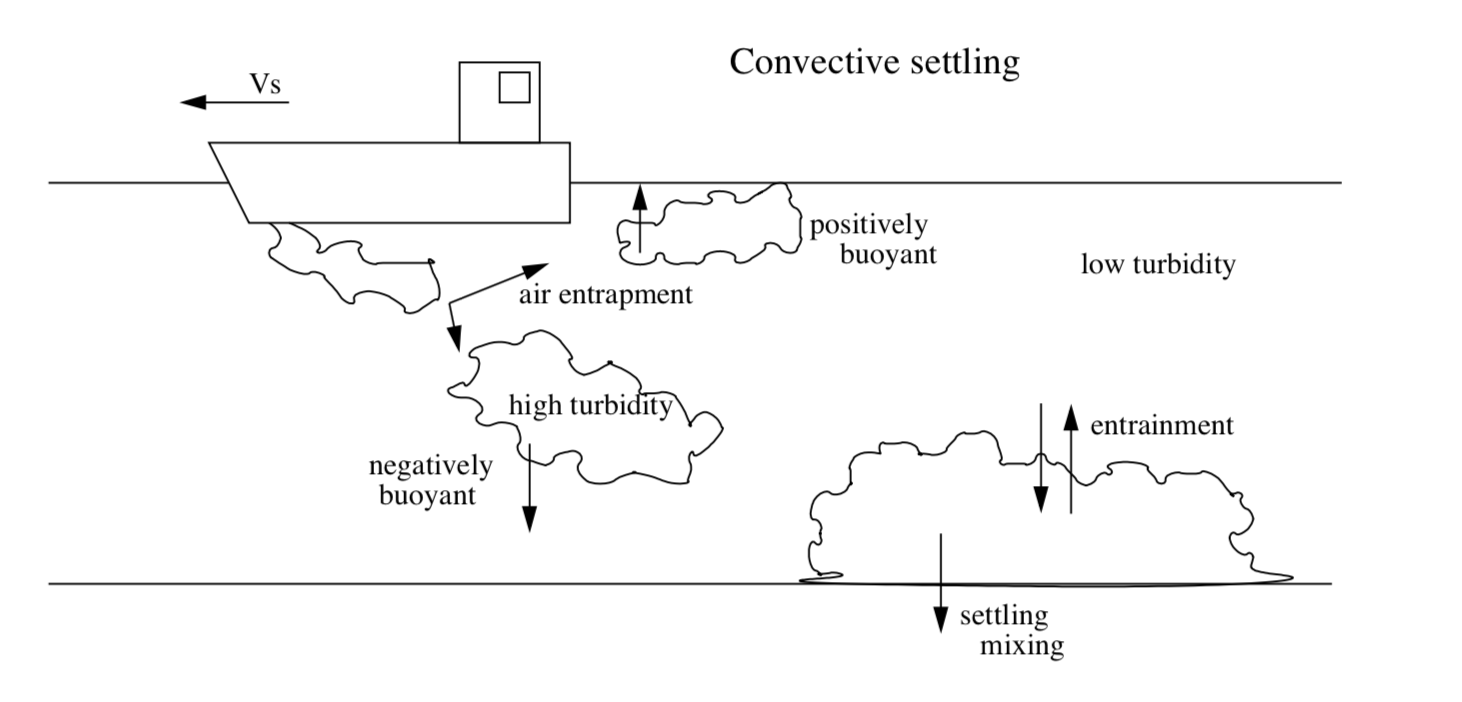
\includegraphics[width=.75\linewidth]{Images/Plume_cloud.png}
    \caption{Plume cloud }
    \label{fig:cloud_plume}
\end{figure}

\newpage
\noindent \textbf{Passive plume} \newline
\noindent
Passive plumes are created due to stripping of dynamic plumes by entrainment caused by turbulence. For example, when the ambient current is strong enough, the plume will be mixed fully with the ambient water. Sediment concentrations are relatively low in a passive plume, therefore fine particles settle extremely slow due to the small settling velocity and the higher depth to the seabed compared to the dynamic plume. The zone of impact of the passive plume is very large and is dependent on the magnitude and direction of the ambient currents. An overview is displayed in figure \ref{fig:passive_plume} \citep{Dankers}.

\begin{figure}[ht!]
    \centering
    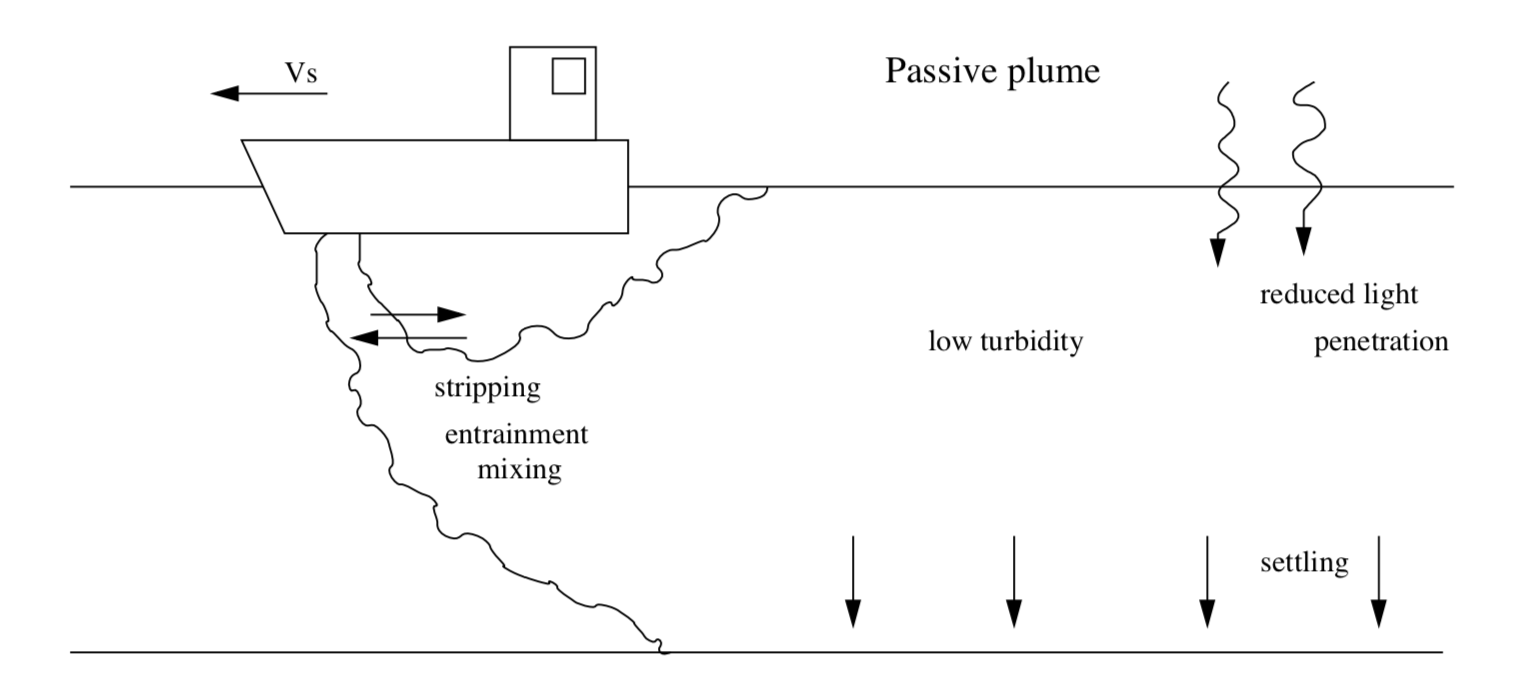
\includegraphics[width=.75\linewidth]{Images/Plume_passive.png}
    \caption{Passive plume phase }
    \label{fig:passive_plume}
\end{figure}




%%%%%%%%%%%%%%%%%%%%%%%%%%%%%%%%%%%%%%%%%%%%%%%%%%%%%%%%%%%%%%%%%%%%%%%%%%%%%%%%%%%%%%%%%%%%%%%%%%%%%%%%%%%%%%%%%%%%%%%%%%%%%%%%%%%%%%%%%%%%%%%%%%%%%%%%%%%%%%%%%%%%%%%%%%%%%%
%Buoyant jet still water Belg 2.3.1
%De wit (2.2) %Belg 2.3.2 
\nomenclature[Z]{JICF}{Jet In Cross Flow}
\label{sec:froudenr}


\section{Turbulent buoyant jet in ambient cross flow}
As mentioned in section \ref{sec:plume}, the outgoing flow of the overflow forms a negative buoyant jet. The ambient current has effect on the buoyant jet, which will be elaborated in this section. In further notice, a dredging plume is noted as an overflow dredging buoyant jet, because it starts with initial buoyancy and momentum where a plume only starts with buoyancy. However, dredging plume fits better in dredging nomenclature.  \newline

\noindent When releasing a momentum- and buoyancy source from a round pipe in ambient fluid with uniform flow velocity and mass density, the round negative buoyant jet in cross flow (JICF) is obtained. As long as the jet starts fully turbulent, mixing of a buoyant JICF is not strongly dependent on the jet Reynolds numbers (Re), but primarily governed by the densimetric Froude number (F$_{\Delta}$) and the jet-to-cross flow velocity ratio ($\lambda$) \citep{Jirka}.

\begin{equation}
\label{eq:Froude}
    F_{\Delta} = \frac{W_0}{\sqrt{D g  \frac{\Delta \rho}{\rho_w}}}
\end{equation}

\begin{equation}
\label{eq:velocity_ratio}
 \lambda = \frac{W_0}{U_{cf}}
\end{equation}
\newline

\nomenclature[A]{$F_\Delta$}{Densimetric Froude number \nomunit{[-]}}
\nomenclature[A]{$W_0$}{Overflow exit velocity \nomunit{$[m/s]$}}
\nomenclature[A]{$U_{cf}$}{Ambient cross flow velocity \nomunit{$[m/s]$}}
\nomenclature[A]{$D$}{Plume source pipe diameter (Overflow outflow diameter) \nomunit{[$m$]}}
\nomenclature[G]{$\Delta \rho$}{Excess mass density of sediment in ambient fluid \nomunit{[$kg/m^3$]}}
\nomenclature[G]{$\rho_w$}{Mass density of water \nomunit{[$kg/m^3$]}}
\nomenclature[G]{$\rho_s$}{Mass density of sediment \nomunit{[$kg/m^3$]}}

\begin{figure}[ht!]
  \centering
    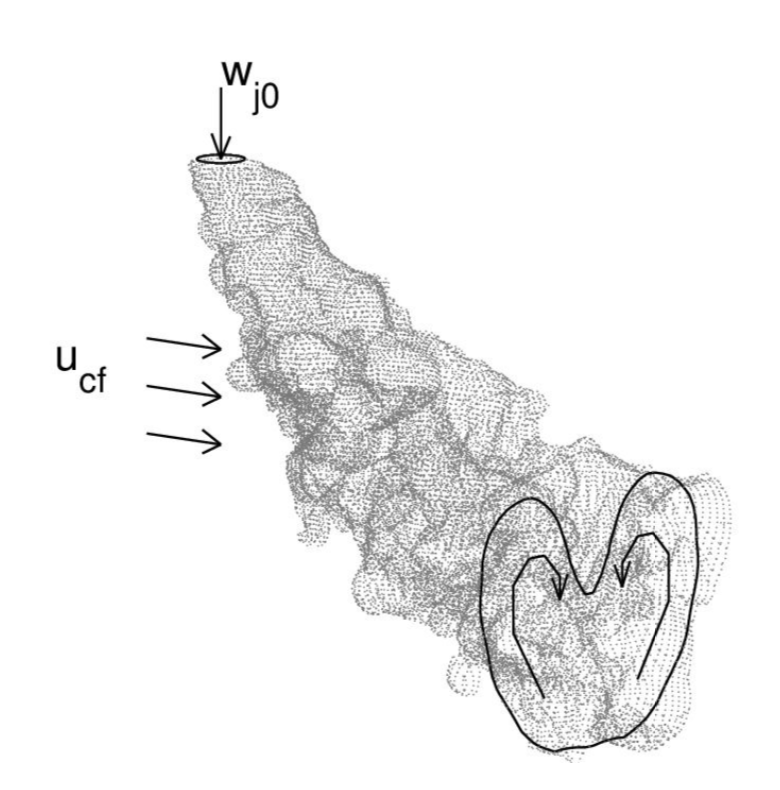
\includegraphics[width=0.4\textwidth]{Images/Jet_mixing.png}
  \caption{Schematic mixing of a negative buoyant JICF }
  \label{fig:Jetmixing}
\end{figure} 

\noindent Where W$_0$ is the overflow exit velocity, U$_{cf}$ is the cross flow velocity (vector sum of dredging speed and ambient current), D the plume source pipe diameter (overflow exit diameter in this case) and $\rho_w$ the mass density of the ambient water. $\Delta \rho$ is the excess mass density of sediment in ambient fluid which also can be described as $\rho_s$ - $\rho$. A schematic overview of mixing of a negative buoyant JICF is shown in figure \ref{fig:Jetmixing} \citep{Dewit}. \newline

\newpage
\noindent The way the plumes spread out is determined by several possible flow regimes \citep{Wright}, \citep{Fischer+}. Jet regime, plume regime and the bent regime are generally found. The jet of a buoyant JICF injected perpendicular to the ambient flow starts with no horizontal velocity. Moving further downstream, the ambient current will take the buoyant plume further in the horizontal. The vertical momentum is important at the exit of the overflow, but eventually buoyancy will take over. \cite{Fischer+} derived length scales to distinguish the different flow regimes of a buoyant JICF. The length scales are given by:

\begin{equation}
\label{eq:lm}
 l_m = \frac{M_0^{3/4}}{B_{0}^{1/2}}
\end{equation}

\begin{equation}
\label{eq:zm}
 z_m = \frac{M_0^{1/2}}{U_{cf}}
\end{equation}

\begin{equation}
\label{eq:zb}
 z_b = \frac{B_0}{U_{cf}^3}
\end{equation}

\begin{equation}
\label{eq:zc}
 z_c = z_m\Big(\frac{z_m}{z_b}\Big)^{1/3} 
\end{equation}

\nomenclature[A]{$B_0$}{Initial overflow buoyancy flux \nomunit{[$m^4/s^3$]}}
\nomenclature[A]{$M_0$}{Initial overflow momentum flux \nomunit{[$m^4/s^2$]}}
\nomenclature[A]{$l_m$}{Jet-to-plume length scale \nomunit{[$m$]}}
\nomenclature[A]{$z_b$}{Buoyancy length scale \nomunit{[$m$]}}
\nomenclature[A]{$z_c$}{Deep water momentum length scale \nomunit{[$m$]}}
\nomenclature[A]{$z_m$}{Momentum length scale \nomunit{[$m$]}}


\noindent $B_0$ is the overflow buoyancy flux and $M_0$ is the overflow momentum flux. As said, the length scales determine the flow regime. If z < $l_m$ from the source, a buoyant jet acts as a jet and when z > $l_m$ the buoyant jet acts as a plume. The length scales $z_m$ \& $z_b$ are defined for the influence of momentum and buoyancy compared to the ambient current. As long as z < $z_m$, initial momentum is dominant over to the ambient current and so the buoyant jet acts like a jet. If z < $z_b$, initial buoyancy is dominant over the ambient current and so acts as plume. \newline
Independent of momentum- or buoyant dominance, a buoyant JICF always ends as a bent over plume due to the horizontal ambient current (figure \ref{fig:Jetmixing}). As long as $z_b$ > $z_m$, the transition to the bent over plume happens after z > $z_b$. In reverse, if $z_m$ > $z_b$, the transition happens after $z_c$. Figure \ref{fig:lengthscales} \citep{Dewit} summaries the length scales and the connected flow regimes of a buoyant JICF, as derived by \cite{Fischer+}.

\begin{figure}[ht!]
    \centering
    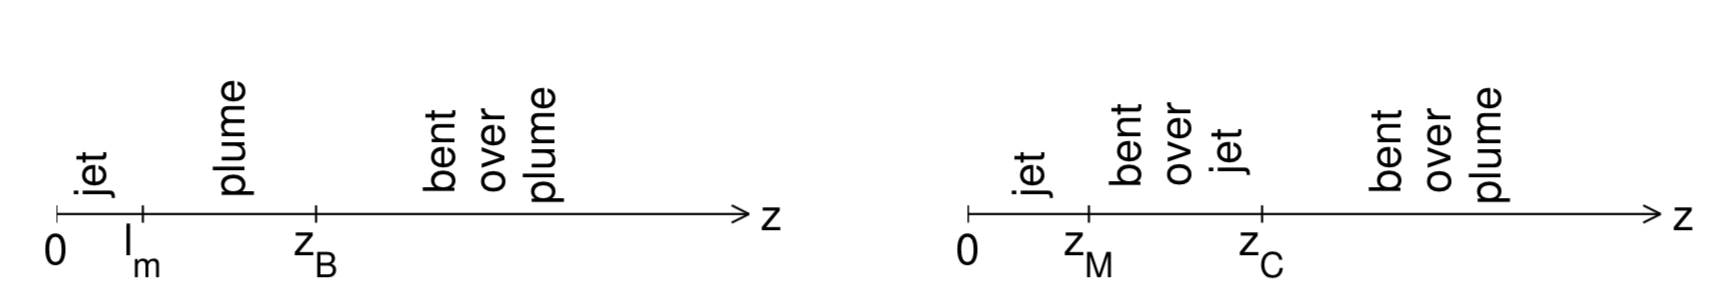
\includegraphics[width=1\linewidth]{Images/Length_scale_z.png}
    \caption{Length scales and flow regimes of a buoyant JICF in case $z_b$ > $z_m$ (left) and in case $z_m$ > $z_b$ (right) }
    \label{fig:lengthscales}
\end{figure}

\noindent The plumes studied in this work correspond to ranges of $F_\Delta$ and $\lambda$ occurring in sediment plumes released from dredging vessels. Even though the initial relative density difference is usually in the order of 1 to 10\%, the buoyancy is relatively weak compared to the cross flow in these cases, with the jet-to-cross flow velocity ratio usually in the range 0.25 < $\lambda$ < 3 \citep{Decrop}. Therefore, the momentum length scale $z_m$ is larger than the buoyancy length scale $z_b$ in most cases, leading to a plume regime sequence as shown in figure \ref{fig:lengthscales} on the right. However, in strong cross flow cases both $z_m$/D and $z_b$/D are around or less than unity, due to which the plume transforms very rapidly to the bent over plume regime.


%%%%%%%%%%%%%%%%%%%%%%%%%%%%%%%%%%%%%%%%%%%%%%%%%%%%%%%%%%%%%%%%%%%%%%%%%%%%%%%%%%%%%%%%%%%%%%%%%%%%%%%%%%%%%%%%%%%%%%%%%%%%%%%%%%%%%%%%%%%%%%%%%%%%%%%%%%%%%%%%%%%%%%%%%%%%%%
%De wit (2.4)

\section{Near field processes dredging plume}

\noindent %\textbf{Near-, mid- and far field dredging plume} \newline
Near field is defined as the zone where plume mixing is dominated by density differences and interaction with the dredging vessel. Typically, the near field zone ends some hundred meters behind the TSHD. In the far field, plume mixing is mainly governed by sediment settling and ambient (tidal) currents \citep{Dewit}. \newline The focus of this study is plume mixing in the near field, because near field mixing determines the amount and distribution of suspended sediment available in the far field. An overview is shown in figure \ref{fig:field}\citep{Dewit}.

\begin{figure}[ht!]
    \centering
    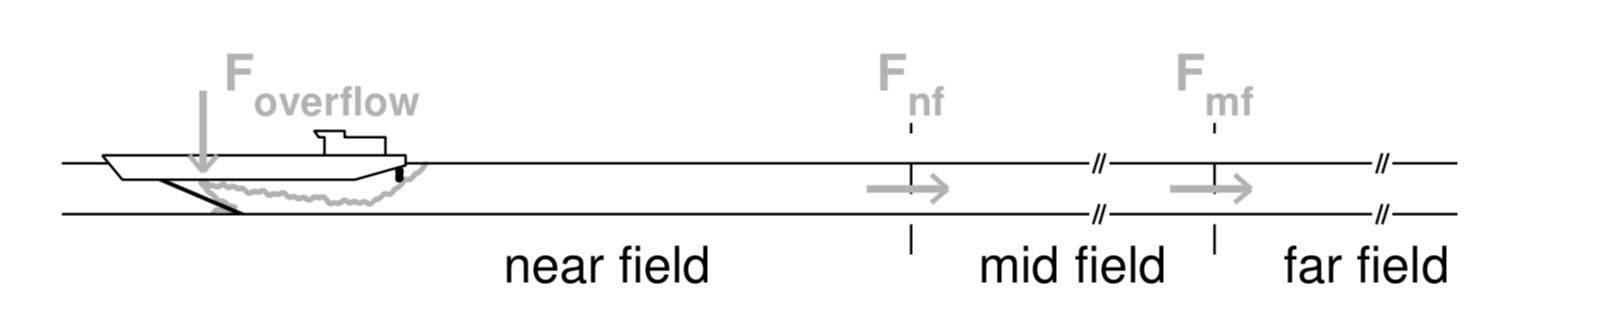
\includegraphics[width=1\linewidth]{Images/Nearfield_Midfield_Farfield.png}
    \caption{Schematic overview of near-, mid- and far field dredging plume. }
    \label{fig:field}
\end{figure}

\noindent The dredge plume normally contains a non-uniform sediment grain size distribution. The sediment particle diameter ($D_p$) can range from sand ($D_p$ > 63 $\mu m$) to mud ($D_p$ < 63 $\mu m$). However, due to the slower settling of finer sediment in the hopper with respect to coarser sediment, the overflow and therefore the exiting plume generally contains more mud and finer particles than the dredged material \citep{Rhee}. \newline
\noindent Under influence of turbulence and differences in settling velocity, mud particles can cluster together to form flocs with typical sizes of 0.01-1mm. The density of mud flocs is less than the density of individual mud particles, however the settling velocity is larger. Flocculation is especially important when the mud concentration is large and therefore strong flocculation has been found for mud fractions inside an overflow plume with floc diameters of 40 - 800$\mu m$ and floc settling velocities of 0.1 - 6mm/s \citep{Smith+}. Even after flocculation, the mud settling velocity is very small leading to large deposition periods, especially for the mud in the surface plume which can take hours to days before it has deposited at the seabed. Although the overflow plume leaves the vessel at the keel several meters below the water surface, the initial velocity is downward and it is denser than the ambient water (it is negatively buoyant). Already close behind the dredger, a part of the overflow plume can end up fully mixed near the water surface as a surface plume where a surface plume can remain visible for considerable distances from a dredger \citep{Newell+}. \newline \newline
\noindent Generally, buoyant JICF mixing is not responsible for the generation of a surface plume, as it will bring the plume further down - not up. Therefore, other processes are responsible for the generation of a surface plume. All theses processes are further elaborated in chapter \ref{CH:influence_factors}.

\nomenclature[A]{$FF_{nf}$}{Near field suspended fine sediment flux (ratio with $FF_{OV}$) \nomunit{[-]}}
\nomenclature[A]{$FF_{mf}$}{Mid field suspended fine sediment flux (ratio with $FF_{OV}$) \nomunit{[-]}}
\nomenclature[A]{$FF_{OV}$}{Suspended fine sediment flux through overflow ($FF_{overflow})$\nomunit{$[kg/s]$}}
\chapter{Influence Factors Turbidity Creation}
\label{CH:influence_factors}
%\textbf{NEARFIELD} \newline
%\textbf{3D CFD modelling}
INTRO MET VERWIJZINGEN

\newpage
\section{Hopper inlet / sedimentation}
%\textbf{Vragen aan vRhee}

As noted in chapter \ref{sec:hopper}, The filling of the hopper basin has certain phases as shown in figure \ref{fig:phases_overflow_loss}. If the basin is almost filled, which is indicated by phase IV in the figure, the overflow losses are grown exponentially. A way to decrease the overflow plume outside of the vessel, is to decrease the amount of sediment-mixture that reaches the overflow. In order to do this, the filling process should show other phases, with example a way to let the overflow loss not grow exponentially in phase IV.

%3D flow profile vragen aan Keetels.











%%%%%%%%%%%%%%%%%%%%%%%%%%%%%%%%%%%%%%%%%%%%%%%%%%%%%%%%%%%%%%%%%%%%%%%%%%%%%%%%%%%%%%%%%%%%%%%%%%%%%%%%%%%%%%%%%%%%%%%%%%%%%%%%%%%%%%%%%%%%%%%%%%%%%%%%%%%%

\nomenclature[Z]{LES}{Large-Eddy Simulation}

\section{Dredging speed}
Dredging speed has an influence to the amount of turbidity at the water surface. This can be related to a low $\lambda$ value (equation \ref{eq:velocity_ratio}) which correlates to a high cross flow velocity ($U_{cf}$). \cite{Decrop} investigated the effect of dredging speed with his numerical LES model with typical operational conditions ($C_0$ =  90 g/l \& $W_0$ =  1.9 m/s). The first simulation is done with an $U_{cf}$ of 1 m/s, for example a dredging vessel trailing to still water with a velocity of 1 m/s. The resulting plume is shown in figure \ref{fig:dredging_speed}, top panel where in this case the bulk of the released sediment moves to the sea bed rapidly, forming a density current and a more dilute surface plume with c/$C_0$ =  $10^{-3.5}$ at x/D = 100.

\begin{figure}[ht!]
    \centering
    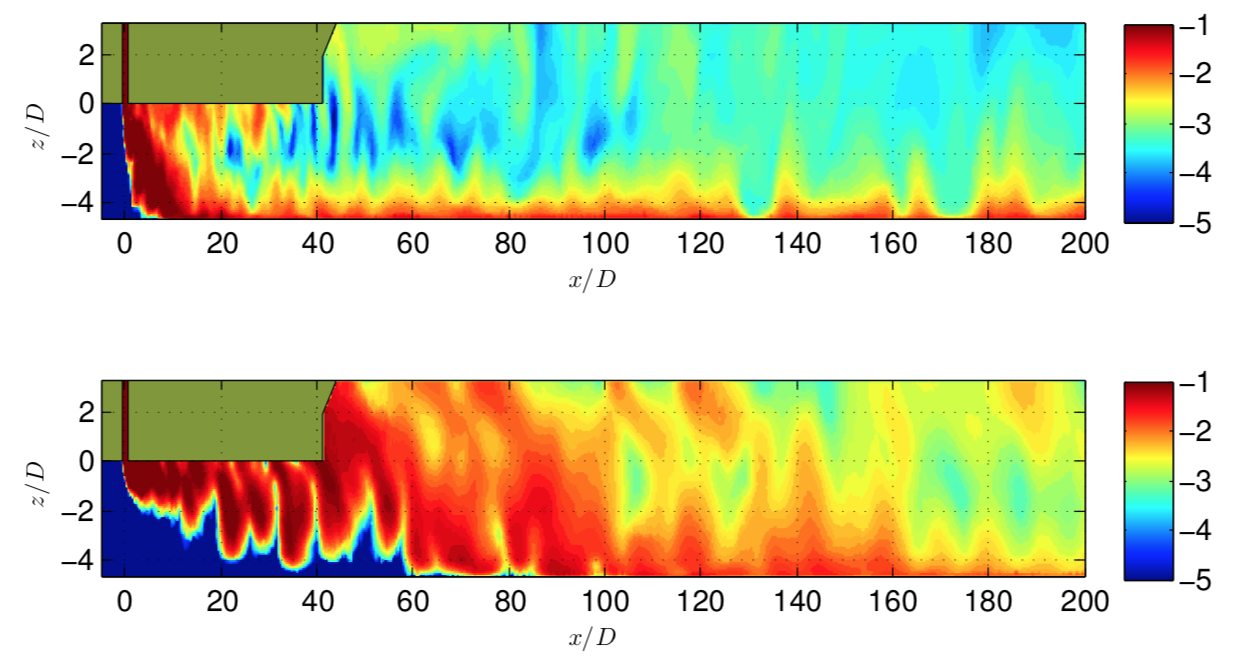
\includegraphics[width = .8\linewidth]{Images/dreding_speed.png}
    \caption{Contours of log C/$C_0$. Top panel: $U_{cf}$ =  1 m/s , lower panel: $U_{cf}$ =  3 m/s}
    \label{fig:dredging_speed}
\end{figure}

\noindent In the second case, the speed through water was increased to $U_{cf}$ = 3 m/s. For example, this situation occurs while trailing with speed over ground of 2 m/s in a current velocity of 1 m/s, head on. The resulting plume is shown in figure \ref{fig:dredging_speed}, lower panel. It is shown that due to the increased $U_{cf}$, a large part of the plume is lifted enough to be caught by the propellers. As a result, a much higher amount of sediment is mixed towards the surface. The sediment concentration in the surface plume is c/$C_0$ =  $10^{-2.5}$ at x/D = 100. A threefold increase in $U_{cf}$ has therefore resulted in a tenfold increase in the surface plume concentration. \newline

\noindent \cite{Dewit} did a comparable experiment to see what dredging speed did to the plume contours underwater. Instead of determining a $U_{cf}$ value, the jet-to-cross flow velocity ratio is determined. A value of $\lambda$ =  1.28 was chosen for normal dredging speed and a value of $\lambda$ =  0.68 for high dredging speed. As figure \ref{fig:dredging_speed_2} describes the two cases, a decrease in jet-to-cross flow velocity ratio clearly increases the surface plume in the near field.

\begin{figure}[ht!]
    \centering
    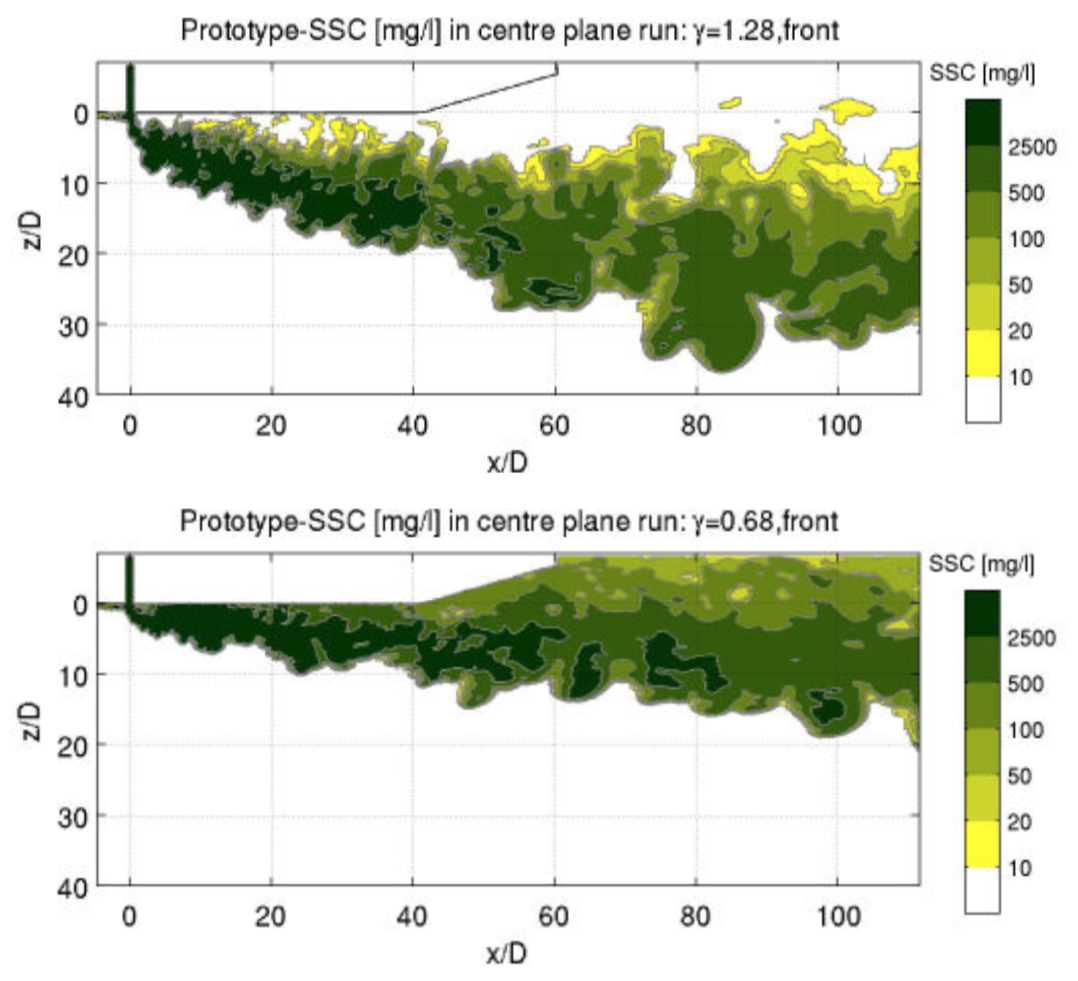
\includegraphics[width = .6\linewidth]{Images/Dredging_speed.png}
    \caption{SSC with normal dredging speed ($\lambda$ = 1.28) and high dredging speed ($\lambda$ = 0.68)}
    \label{fig:dredging_speed_2}
\end{figure}

\noindent In addition, as can be seen from figure \ref{fig:dredging_speed_3}, a difference in horizontal spreading is visible. A high dredging speed will decrease the horizontal spreading of the plume with a more dense packed plume \citep{Dewit}.

\begin{figure}[ht!]
    \centering
    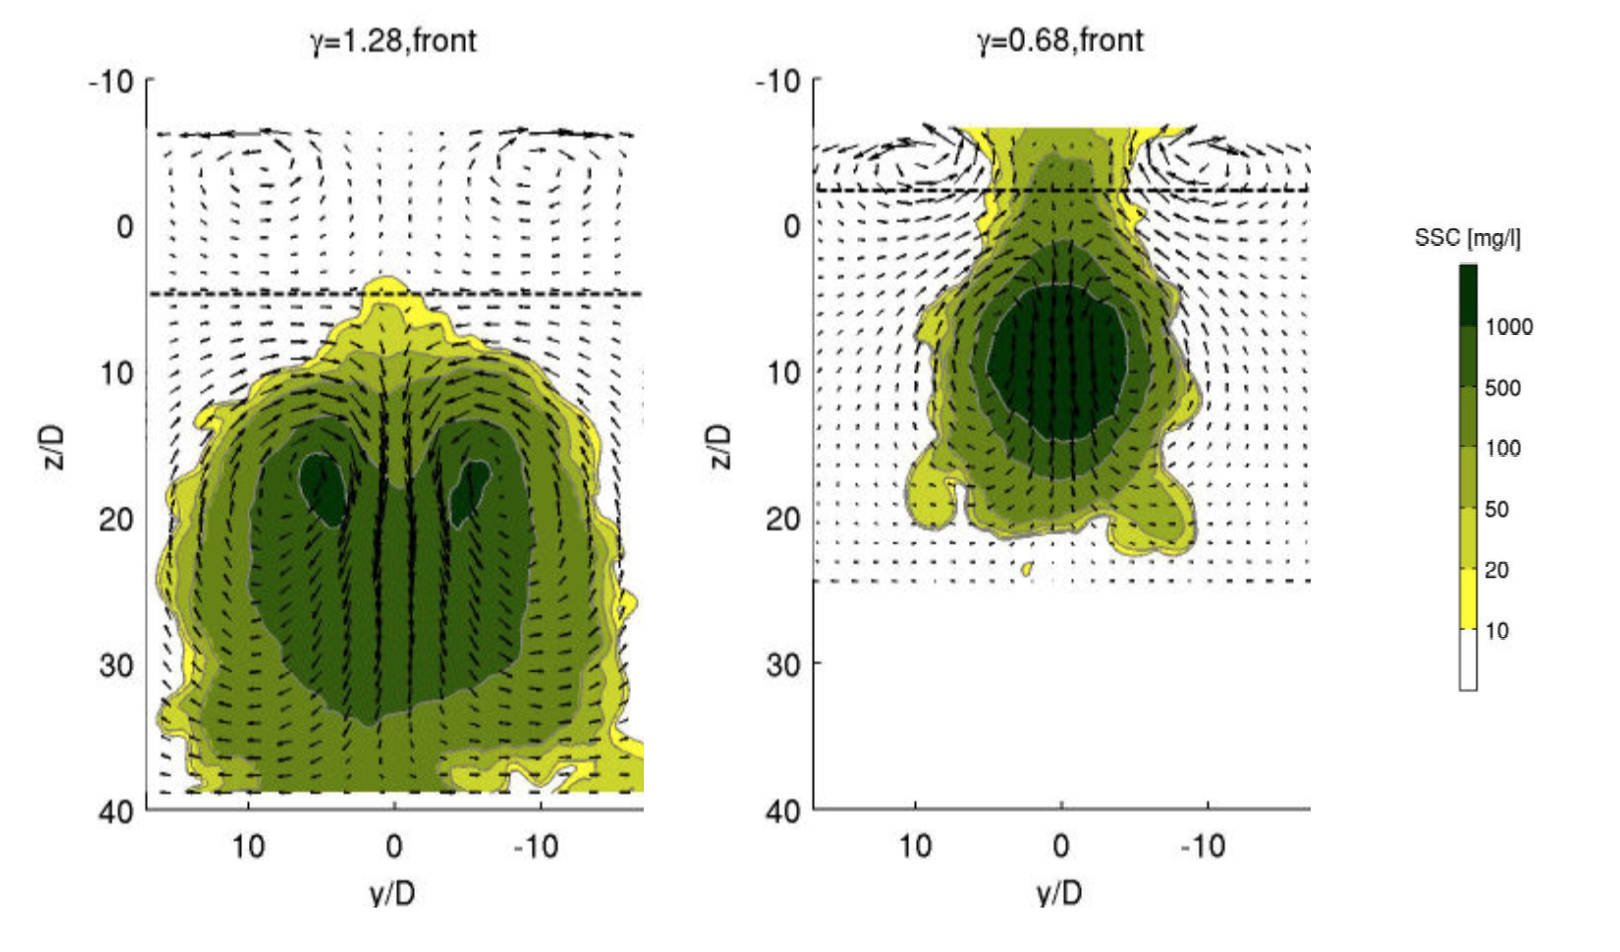
\includegraphics[width = .8\linewidth]{Images/Dredging_Speed_width.png}
    \caption{SSC at x = 100D with normal dredging speed (left) and high dredging speed (right)}
    \label{fig:dredging_speed_3}
\end{figure}











%%%%%%%%%%%%%%%%%%%%%%%%%%%%%%%%%%%%%%%%%%%%%%%%%%%%%%%%%%%%%%%%%%%%%%%%%%%%%%%%%%%%%%%%%%%%%%%%%%%%%%%%%%%%%%%%%%%%%%%%%%%%%%%%%%%%%%%%%%%%%%%%%%%%%%%%%%%%


\nomenclature[A]{$H_k$}{Depth below the keel \nomunit{[-]}}
\nomenclature[Z]{VIF}{Vertical Distribution of flux of fines}

\section{Dredging / water depth}

In figure \ref{fig:depth_belg}, vertical profiles of $C$/$C_0$ are given at y = 0 and x/D = 100 and horizontal profiles are shown in the surface plume at y = 0 and at 0.5m below the surface. It can be observed that the case with keel clearance ($H_k$) of 5m differs substantially from the other cases. The sediment concentration in the surface plume is about 4 times higher at x/D = 100. In the horizontal profile, the concentrations are similar for the cases with $H_k$ $\geq$ 9m, but for $H_k$ = 5m the surface concentration increases significantly at about x/D = 60. This location is at 30-40m behind the propellers \citep{Decrop}. Concluding figure \ref{fig:depth_belg}, water depth does influence the sediment concentration in suspension for $H_k$ $\geq$ 9m, but does not influence the sediment concentration at the water surface.

\begin{figure}[ht!]
    \centering
    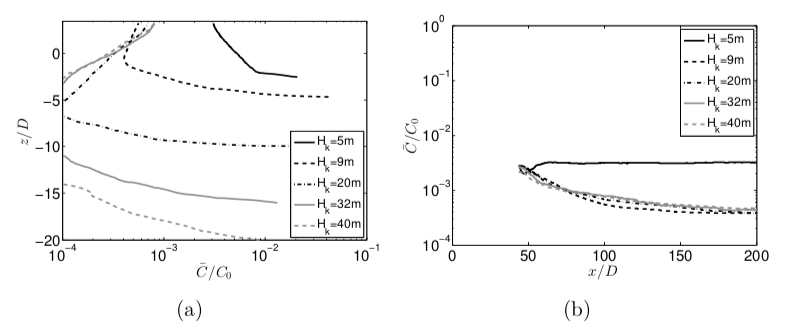
\includegraphics[width = 0.9\textwidth]{Images/depth_belg.png}
    \caption{Time-averaged sediment concentration $C$/$C_0$, for identical cases except for the different keel clearance $H_k$. In figure (a), vertical profiles are given at y = 0 and x/D = 100. In figure (b), horizontal profiles are given at y = 0 and at 0.5m below the surface.}
    \label{fig:depth_belg}
\end{figure}

\noindent In figure \ref{fig:depth_belg_2}, the streamwise velocity at y = 0 is shown for two keel heights calculated by the LES model of \cite{Decrop}. The difference in streamwise velocity is very noticeable where with decreasing water depth, the streamwise velocity distribution becomes less broad, with large areas with higher velocities.

\begin{figure}[ht!]
    \centering
    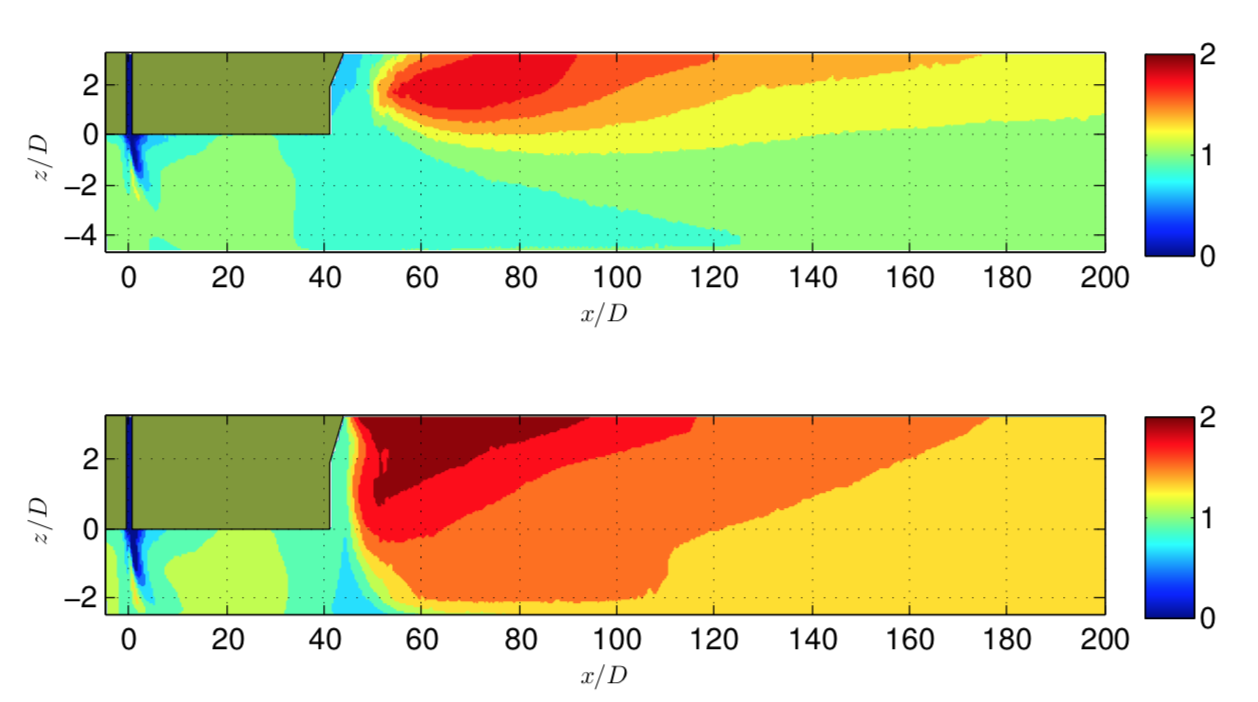
\includegraphics[width = 0.9\textwidth]{Images/depth_velocity_belg.png}
    \caption{Time averaged streamwise velocity at y = 0. top: $H_k$ = 9m, bottom: $H_k$ = 5m}
    \label{fig:depth_belg_2}
\end{figure}



\newpage
\noindent \cite{Dewit} calculated the vertical distribution of flux of fines in suspension (figure \ref{fig:depth_dewit}) to illustrate the effects of near field conditions like dredging speed, water depth, pulsing and air entrainment. All vertical distributions for situations with low $U_{cf}$ and large depth are strongly concave with the majority of the flux near the bed. For runs with large $U_{cf}$ or smaller depth the curves are less concave. For the smallest depth = 12m all curves are near linear, independent of air, pulsing or $U_{cf}$. A linear curve indicates a vertically fully mixed plume. The cases with lower density show a higher vertical distribution comparing to the higher density, which indicates that more particles found higher in the water column which makes sense with a lower density. \newline \noindent 

\begin{figure}[ht!]
    \centering
    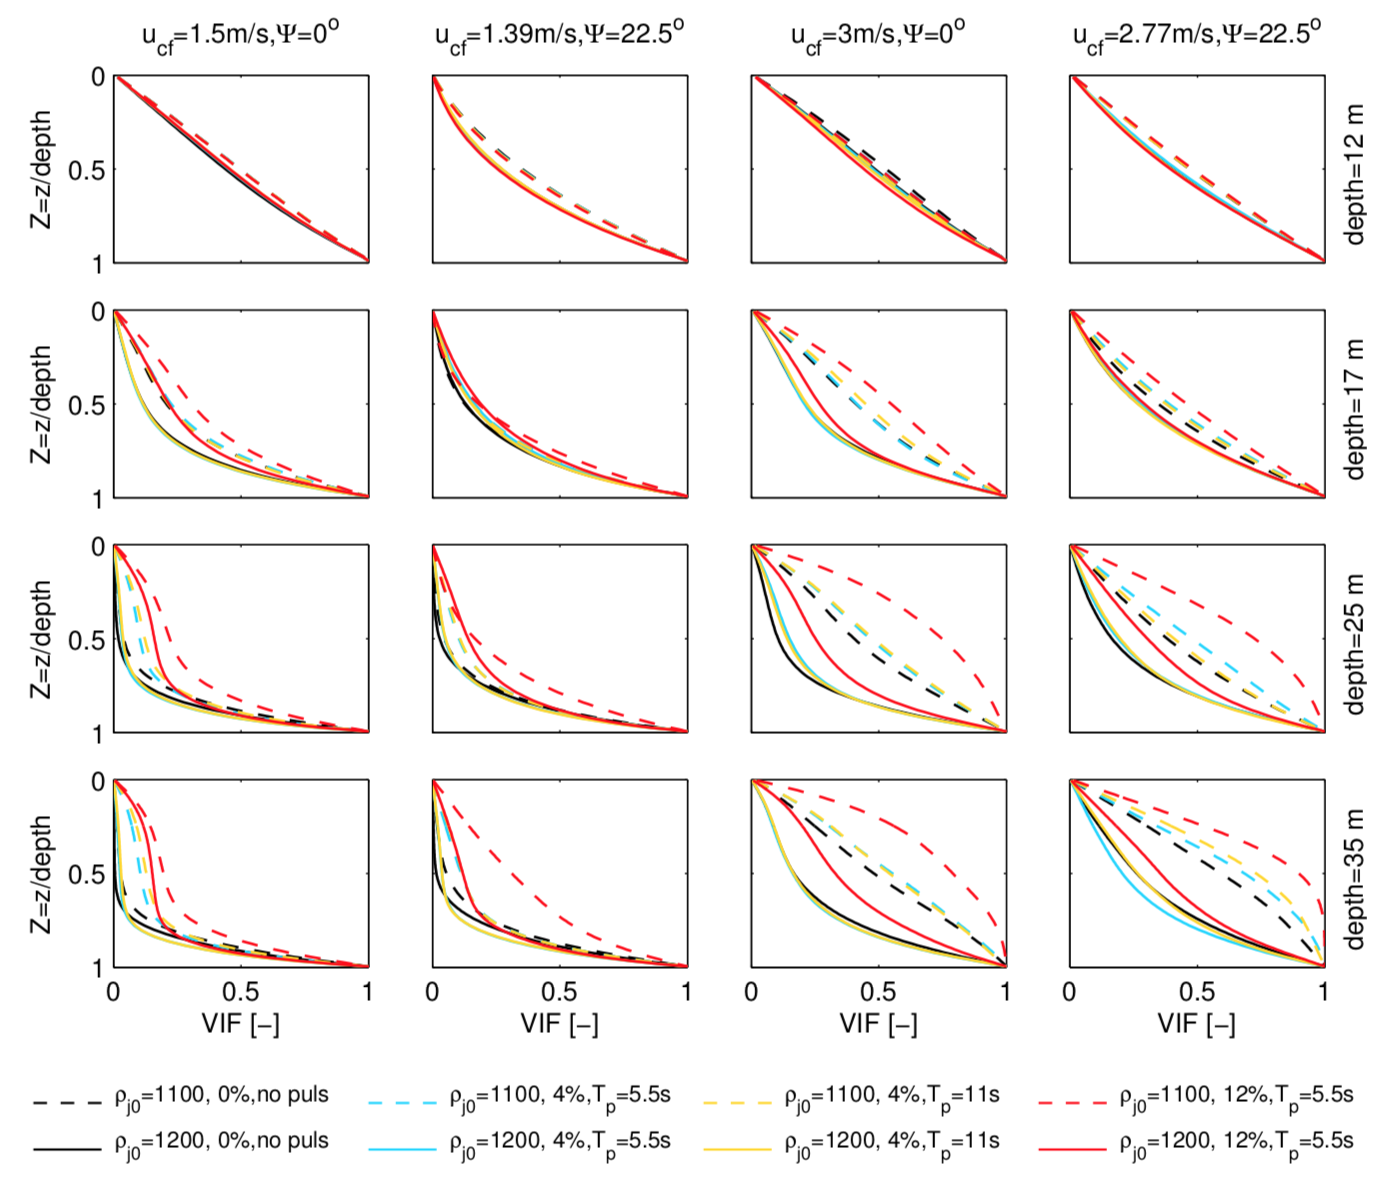
\includegraphics[width = 1\textwidth]{Images/Dredging_depth.png}
    \caption{Vertical distribution of the flux of fines (VIF =  $\int_{0}^{Z}$ 0Z flux dZ / $\int_{0}^{1}$ flux dZ, with Z =  z/depth) at the end of near field x =  350m}
    \label{fig:depth_dewit}
\end{figure}










%%%%%%%%%%%%%%%%%%%%%%%%%%%%%%%%%%%%%%%%%%%%%%%%%%%%%%%%%%%%%%%%%%%%%%%%%%%%%%%%%%%%%%%%%%%%%%%%%%%%%%%%%%%%%%%%%%%%%%%%%%%%%%%%%%%%%%%%%%%%%%%%%%%%%%%%%%%%
\newpage
\section{Angle between TSHD and ambient current}

A high cross flow velocity leads to a larger plume flux still in suspension after a certain settling time, more sediment in higher parts of the water column and thus a large surface plume. A high cross flow velocity increases the interaction between the plume and the TSHD hull and the plume and the TSHD propellers. When a TSHD is sailing under an angle with the ambient current, the overflow plume is pushed towards the side of the TSHD hull where it can be taken along by the expanding flow towards the free surface. The more the ambient current comes from the side, the more surface plume can be expected\citep{Dewit}. When looking at figure \ref{fig:depth_dewit}, dredging under an angle $\psi$ =  22.5$^\circ$ to the ambient velocity gives lifted vertical distribution profiles with more material in the upper parts of the water column than for $\psi$ =  0$^\circ$. The one exception is the case with depth =  12m where $U_{cf}$ =  1.39m/s, $\psi$ =  22.5$^\circ$ has a lower vertical distribution profile than $U_{cf}$ = 1.5m/s, $\psi$ = 0$^\circ$.

\begin{figure}[ht!]
    \centering
    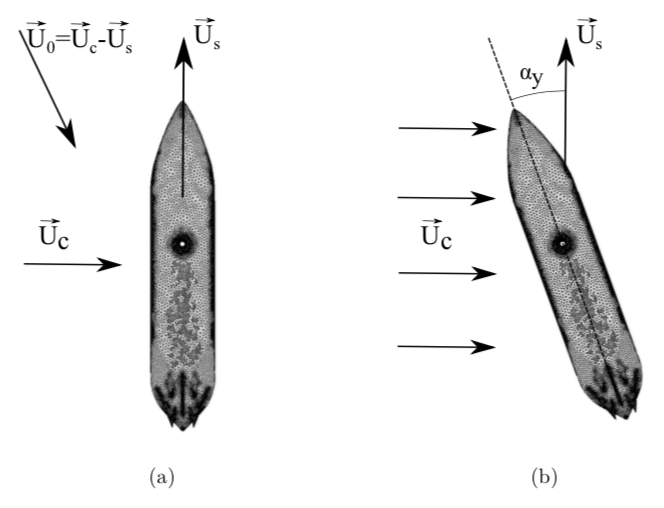
\includegraphics[width = .6\linewidth]{Images/Anlge_TSHD.png}
    \caption{(a) Modeling approach for a ship in a cross current: the through-water velocity $U_0$ is equal to the cross current velocity vector $U_c$ minus the ship’s course vector $U_s$. (b) Definition of the yaw angle $\alpha_y$ of a ship sailing in a cross current.
}
    \label{fig:Angle_TSHD}
\end{figure}


\noindent \cite{Decrop} simulated a TSHD sailed at $U_s$ = 0.9 m/s (over ground) in a perpendicular cross current of $U_c$ = 0.45 m/s. See figure \ref{fig:Angle_TSHD}a for a sketch. This results in a net speed through water of $U_{0}$ = 1 m/s and an angle between the ship center line and its speed through water of $\psi$ = 26.6$^\circ$. In the LES model, the ship is considered stationary with its center line along the x-axis and the net current is imposed at the boundary. The angle of 26.6$^\circ$ is, however, an overestimation. Indeed, for a ship to follow its course in a cross current, it must develop some yaw angle. A ship’s yaw angle is the angle between the course and the vessel center line (figure \ref{fig:Angle_TSHD}b). When a ship is sailing in a cross current, its yaw angle or drifting angle $\alpha_y$ is estimated by \cite{Pianc}.

\nomenclature[A]{$U_0$}{Ambient cross flow velocity \nomunit{[$m/s$]}}

\begin{equation}
    tan (\alpha_y) =  \frac{U_c}{U_s}
\end{equation}


\noindent This equation returns exactly the same angle as initially found for the angle between the ship center line and the velocity vector relative to the water, $U_0$. This means a ship would always align itself with the relative velocity $U_0$. A TSHD with drag head on the sea bed has some kind of anchoring, due to which $\alpha_y$ might be smaller than atan(Uc/Us). However, setting the angle $\alpha$ simply to atan($U_c$/$U_s$) is not correct. The angle between a ship and its speed through water will be much lower. In this sense, the simulation with $\psi$ = 26.6°corresponds with a situation with a cross flow significantly stronger than 0.45 m/s, or with an anchored TSHD serving as a barge for cutter dredgers. The other plume boundary conditions were set to $C_0$ = 55 g/l and $W_0$ = 1.9 m/s. \newline \newline
\noindent When looking at the time-averaged $C$/$C_0$ in a cross section (x/D = 50), it can be observed that the plume is asymmetric (figure \ref{fig:Angle_TSHD2}, top panel). It can be seen that the surface plume is situated around y/D = 15 at x/D = 50. The angle of the path of the surface plume is therefore about atan(15/50) = 16.7°. This is lower than the angle between the ship and the relative velocity $U_0$. The near-bed density current is positioned around y/D = 30, corresponding to a path angle of atan(30/50) = 31°. This is larger than the angle of the relative velocity $U_0$. The density current and the surface plume clearly feel the influence of the cross current in a different way. In order to analyze this situation, a detailed three-dimensional visualization is needed.
The resulting surface plume and subsurface density current are shown in figure \ref{fig:Angle_TSHD2}, lower panel. It can be seen that the density current follows another angle compared to the surface plume. The descending density current feels a secondary current induced by the angle between ship and flow. Therefore the density current is diverted towards a higher angle than the cross flow (towards the left of the figure).

\begin{figure}[ht!]
    \centering
    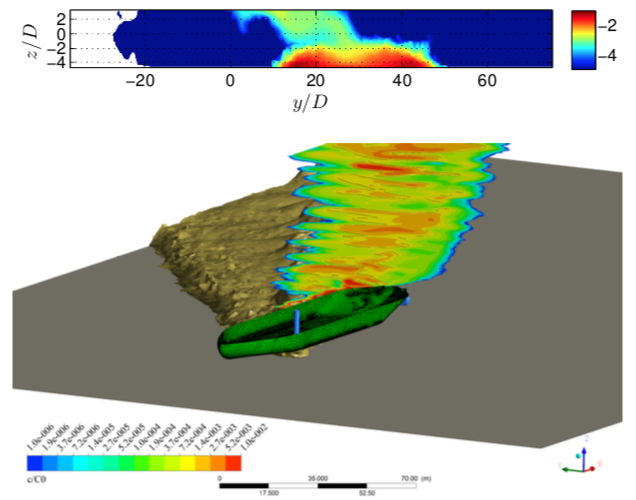
\includegraphics[width = .7\linewidth]{Images/Angle_TSHD2.png}
    \caption{TSHD sailing in a cross flow. Top panel: Vertical cross section of time-averaged sediment concentration field log($C$/$C_0$) at x/D = 50. Lower panel: Surface plume concentration $c$/$C_0$ in colour scale and density current in brown iso-surface.
}
    \label{fig:Angle_TSHD2}
\end{figure}

\noindent The question is now whether the surface plume in a cross flow has significantly different concentration levels as compared to a plume without cross flow. In figure \ref{fig:Angle_TSHD3}, the instantaneous concentration log($C$/$C_0$) for a plume without cross flow and for the same plume with a cross flow is shown. The concentration levels in the surface plumes are very similar. The surface plume in the cross flow case is wider and has a larger variation in $C$. It can be calculated, however, that the total sediment flux in both plumes is quite similar \citep{Decrop}. But as can be seen in figure \ref{fig:Angle_TSHD3}b, a higher concentration at the surface can be seen at higher x/D values compared to no cross flow like in figure \ref{fig:Angle_TSHD3}a. A diverted flow will interact with the hull, where a flow towards the surface is present due to the movement of the vessel. Sediment can be taken along with this flow, which will increase the surface plume \citep{Dewit}.


\begin{figure}[ht!]
    \centering
    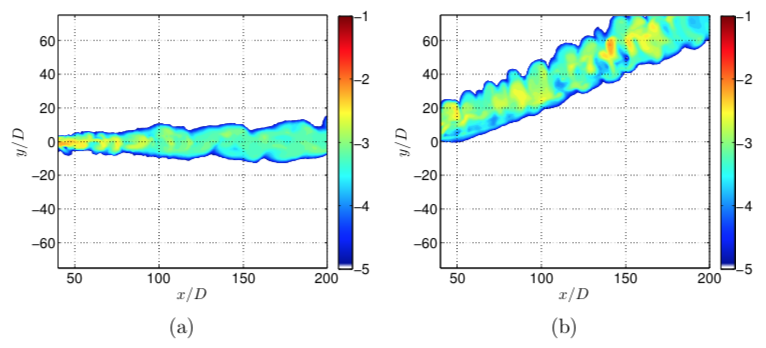
\includegraphics[width = .75\linewidth]{Images/Angle_TSHD3.png}
    \caption{Instantaneous concentration log($c$/$C_0$) for a plume without cross flow (a) and for the same plume with a cross flow (b).
}
    \label{fig:Angle_TSHD3}
\end{figure}










%%%%%%%%%%%%%%%%%%%%%%%%%%%%%%%%%%%%%%%%%%%%%%%%%%%%%%%%%%%%%%%%%%%%%%%%%%%%%%%%%%%%%%%%%%%%%%%%%%%%%%%%%%%%%%%%%%%%%%%%%%%%%%%%%%%%%%%%%%%%%%%%%%%%%%%%


\nomenclature[Z]{SSC}{Suspended Sediment Concentration}
\nomenclature[A]{$St$}{Strouhal number \nomunit{[-]}}
\nomenclature[A]{$T_p$}{Pulsing period \nomunit{[$s$]}}


\section{Pulsing}
A pulsing, discontinuous flow (also shortly treated in section \ref{sec:plume}) in the overflow has been measured on a field trip \citep{Dewit}. The pulsing frequency is dependent on the ambient wave period and the dynamic motions of the TSHD. Pulsing has two effects on the dredging plume: it enhances vertical spreading of the plume and it gives a deeper plume path. The deeper plume path is caused by the extra initial inflow momentum compared to a continuous non-pulsed case with similar volume flux. Pulsing can either enhance the formation of a surface plume by the increased vertical spreading or reduce the formation of a surface plume by the deeper plume path which reduces the influence of the TSHD hull and propellers. For a high cross flow velocity it is found that pulsing results in a smaller surface plume and for a low cross flow velocity pulsing results in a larger surface plume \citep{Dewit}. \newline 
\noindent \cite{Dewit} used a pulsing period ($T_p$) based on a frequency in the range of the Strouhal number ($fD / U_0$) to determine the fluctuation inflow of the overflow. Figure \ref{fig:pulsing} shows three cases with different pulsing periods depending on the Strouhal number. Where a St = 0.27 describes the smallest pulsing period, St = 0.18 describes the middle pulsing period and St = 0.12 describes the largest pulsing period. \newline

\begin{figure}[ht!]
    \centering
    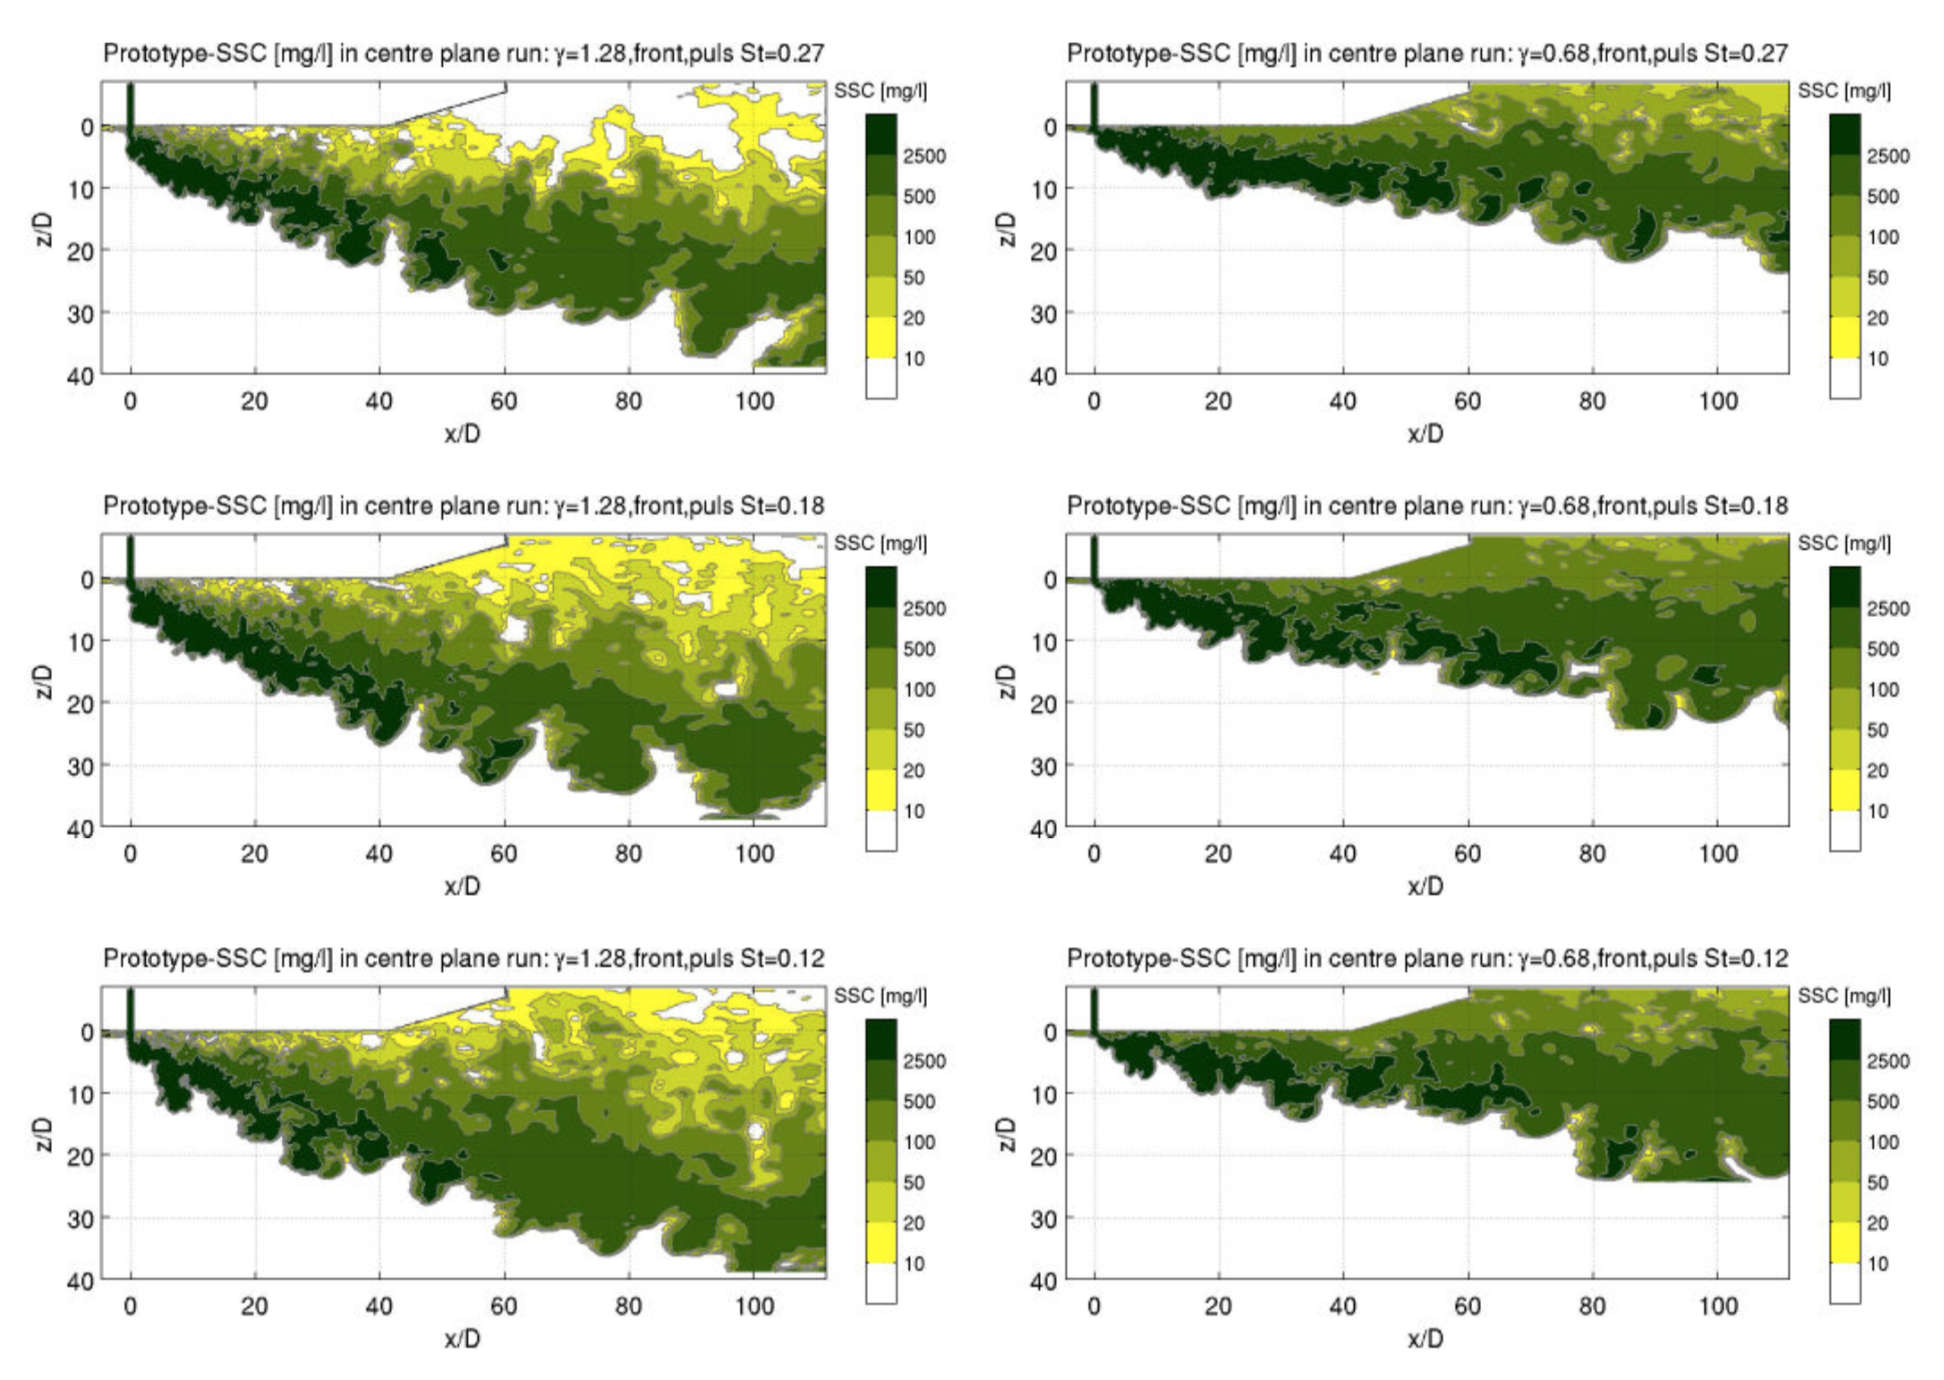
\includegraphics[width = 1\textwidth]{Images/Pulsing.png}
    \caption{SSC with pulsing}
    \label{fig:pulsing}
\end{figure}

\nomenclature[G]{$\lambda$}{Jet-to-cross flow velocity ratio \nomunit{[-]}}

\noindent Figure \ref{fig:pulsing} describes the effect of pulsing on the SSC near field. The left figures describe a normal dredging speed were the right figures describe a high dredging speed and so low $\lambda$ value. As can be seen of the three right figures, the pulsing period does not have a large effect with a high dredging speed: a significant surface plume is visible. Looking at the normal dredging speed, the pulsing period does have a large influence on the SSC. For the largest pulsing period, the separate puffs including gaps can be recognized. More general, a larger pulsing period increases the surface plume. \newline \noindent
When looking at figure \ref{fig:depth_dewit}, air with pulsing lifts the vertical distribution profile up with a small effect of 4\% with $T_p$ =  5.5s or $T_p$ =  11s pulsing and a big effect of 12\% air with $T_p$ =  5.5s. The runs with depth = 25m or 35m, $\rho_{j0}$ =  1100kg/m3 and 12\% air with pulsing even show convex curves: more than 50\% of the fines flux still in suspension can be found in the upper half of the water column and the plume is floating above the bed without touching it \citep{Dewit}.










%%%%%%%%%%%%%%%%%%%%%%%%%%%%%%%%%%%%%%%%%%%%%%%%%%%%%%%%%%%%%%%%%%%%%%%%%%%%%%%%%%%%%%%%%%%%%%%%%%%%%%%%%%%%%%%%%%%%%%%%%%%%%%%%%%%%%%%%%%%%%%%%%%%%%%%%

\nomenclature[Z]{LPM}{Liters Per Minute}
\section{Air}
\label{sec:air}
When the water level inside the vertical overflow shaft is much lower than the water level inside the hopper, the overflowing water forms a plunging jet in the shaft and significant amounts of air can be entrained into the overflow plume. So, the air entrainment and pulsing of the overflow are closely related. There is experimental evidence that a main plume and the air content of this plume will separate into two separate plumes at a certain distance from the source \citep{Zhang+}. The experimental setup is shown in figure \ref{fig:Zhang_experiment}.

\begin{figure}[ht!]
    \centering
    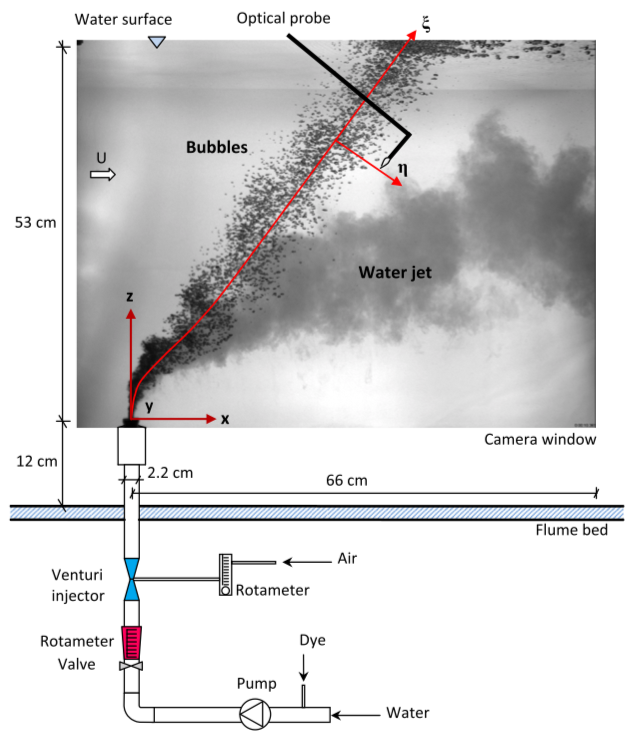
\includegraphics[width = 0.5\textwidth]{Images/Zhang_experiment.png}
    \caption{Schematic side view of the experimental setup (the optical probe drawn in a larger scale), with indication of coordinate system and camera window}
    \label{fig:Zhang_experiment}
\end{figure}
\noindent
In this study, a total of 12 experimental scenarios were investigated (see figure \ref{fig:Zhang_experiment_2}): the air flow rate $Q_a$ at the nozzle was set to be 1, 3 and 5LPM; and the water flow rate $Q_w$ was 0, 1, 3 and 5LPM. Experiments are identified with two numbers: the first and second number are for $Q_a$ and the $Q_w$, respectively. To visualize the trajectories of the liquid-phase in bubbly jets, dye was injected into the water pipeline upstream of the water pump \citep{Zhang+}. 


\begin{figure}[ht!]
    \centering
    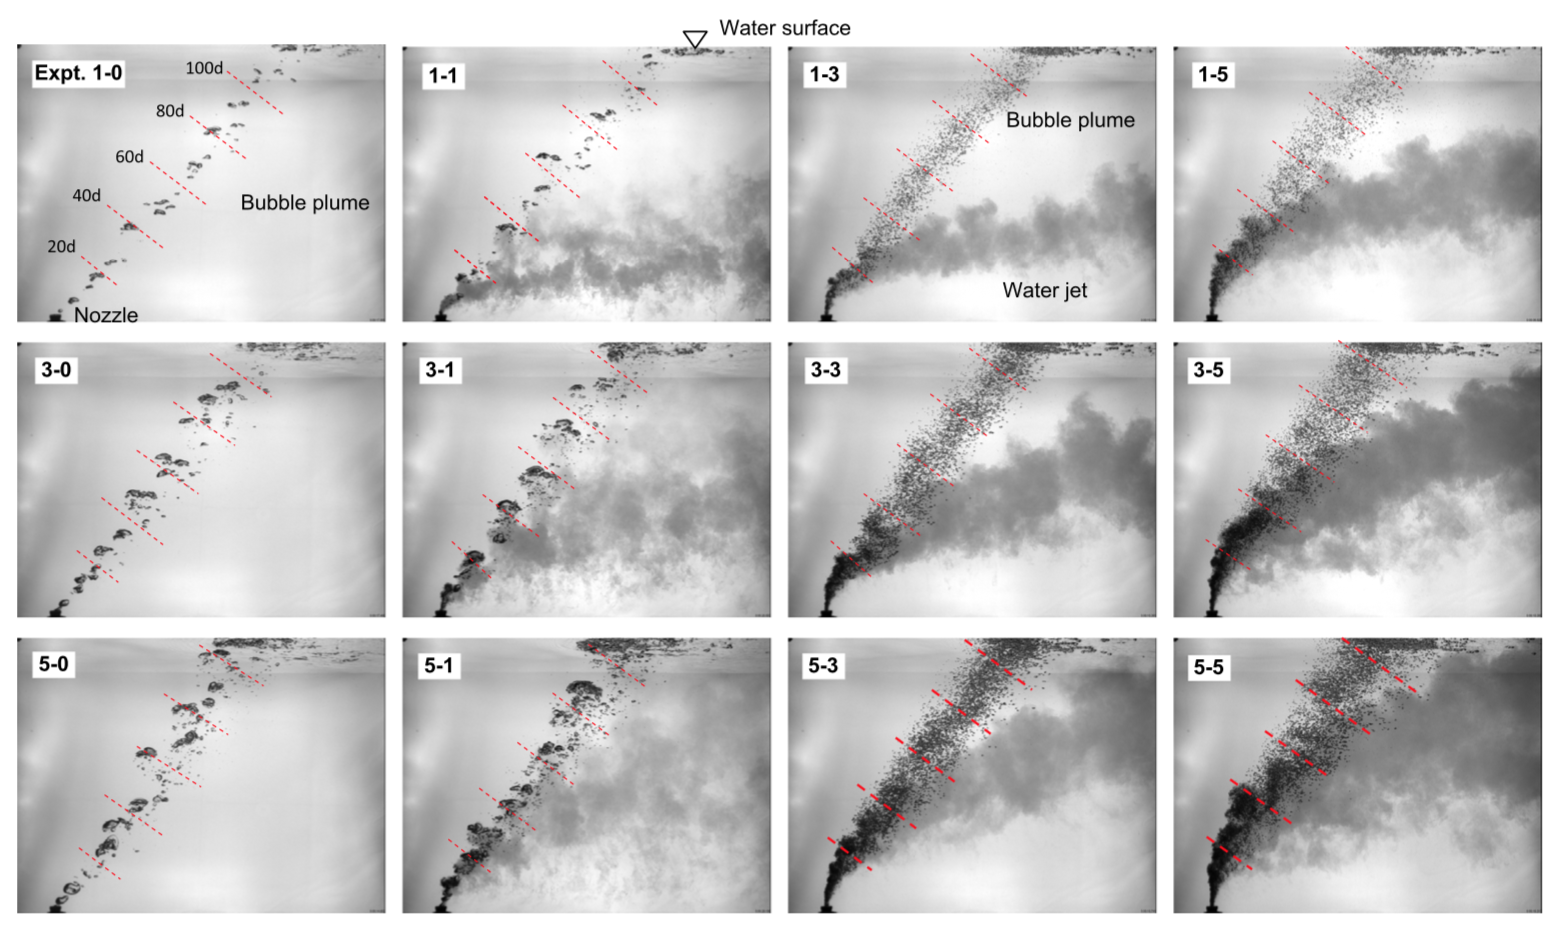
\includegraphics[width = 1\textwidth]{Images/Zhang_experiment_2.png}
    \caption{Photos of bubbly jets in 12 experimental conditions; side view, the first and second numbers in the experiment scenarios represent the air and water discharges at the nozzle (unit: LPM), respectively}
    \label{fig:Zhang_experiment_2}
\end{figure}
\newpage
\noindent As clearly can be seen, when a mixed jet with both air- and water discharge is injected, the jet splits in a clear air path and water path. The separation height appears to increase with the increase in $Q_a$ or $Q_w$, e.g., it increases from approximately section 20d in experiment 1–3 to section 40d in experiment 3–3 and further to Section 60d in experiment 5–3; and it increases from below section 20d in experiment 1–1 to section 20d in experiment 1–3 and further to section 40d in experiment 1–5. The increase of separation height can be explained by the increase of the liquid jet momentum at the nozzle exit \citep{Zhang+}. \newline

\noindent Connecting this to dredging on a TSHD with overflow losses, the influence of air creates a uprising buoyant flow to the water surface which can pick up fine particles and so create a surface plume. Under the influence of gravity, air bubbles are rising, which can be seen as a negative (upward) settling velocity. The terminal rising velocity of air bubbles is reached when buoyancy and drag reach equilibrium. The relation between the terminal air bubble rise velocity and air bubble diameter for still water from \cite{Clift+} for fresh water and from \cite{Chanson+} for fresh water and sea water are presented in figure \ref{fig:bubble_rise}.

\begin{figure}[ht!]
    \centering
    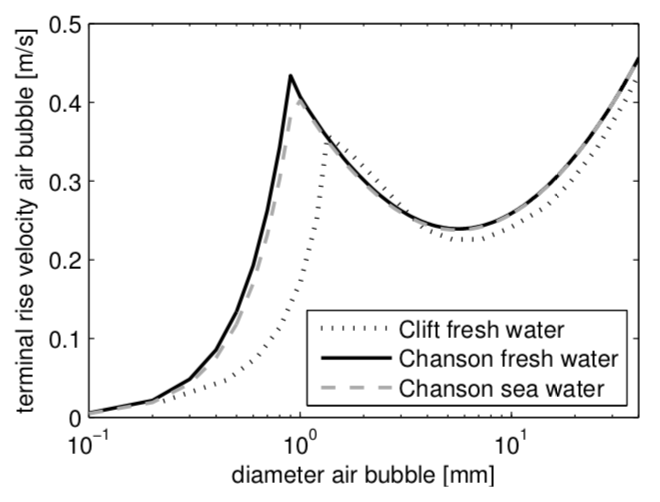
\includegraphics[width = 0.5\textwidth]{Images/bubble_rise.png}
    \caption{Terminal air bubble rise velocity in 20$^{\circ}$C water}
    \label{fig:bubble_rise}
\end{figure}

\noindent The difference between the air bubble rise velocity in fresh water and in sea water for similar bubble diameter is negligible. However, air bubbles created at a plunging jet in sea water are finer than in fresh water, air bubble fusion is reduced and less air volume is entrained: in a scale experiment of a plunging jet with a nozzle diameter of 12.5 mm \cite{Chanson2006+} found a wide variety in air bubbles chord lengths of < 0.5 mm to > 10 mm for fresh and sea water with a smaller mean air bubble chord length in sea water of 3 to 6 mm compared to the mean air bubble chord length of 4 to 7 mm in fresh water. \newline 
\noindent The smaller air bubble size and lower air volume entrainment in sea water can partly be explained by physical properties as density, viscosity, salinity and surface tension, but these physical properties cannot explain all observed differences. Sea water also gives less air entrainment and smaller bubble sizes than saline water, therefore additional differences as organic matter and living organisms (e.g. plankton, algae) must play a role as well \cite{Chanson2006+}. In a fresh water full scale experiment of a drop shaft with a drop height of 1.7 m, bubble chord sizes of <0.5 to >25 mm are measured with mean values of 8 to 10 mm in the drop shaft below the water line and mean values of 2 to 5 mm in the horizontal outflow channel \citep{Chanson}. \newline
The overflow of a TSHD is a sand-mud-water mixture drop shaft with drop heights in the order of 0 to 3 m. Dredging often takes place at sea, therefore smaller air bubble sizes are expected than in the experiment of \cite{Chanson} with fresh water. Based on the results of \cite{Chanson2006+} and \cite{Chanson} air bubbles in the overflow are expected to have diameters of <0.5 to >25 mm with a mean diameter in the range of 1 to 9 mm. The sea water air bubble rise velocity for bubble sizes of 1 to 9 mm is 0.4 to 0.24 m/s. \newline

\noindent \cite{Dewit} used these references in his LES model. Figure \ref{fig:air_dewit} shows the difference between 0\% air entrainment (left figure) and 12\% air entrainment with $T_p$ = 5.5s (right figure) at x = 350m, what is declared as the end of the near field of the model. 

\begin{figure}[ht!]
    \centering
    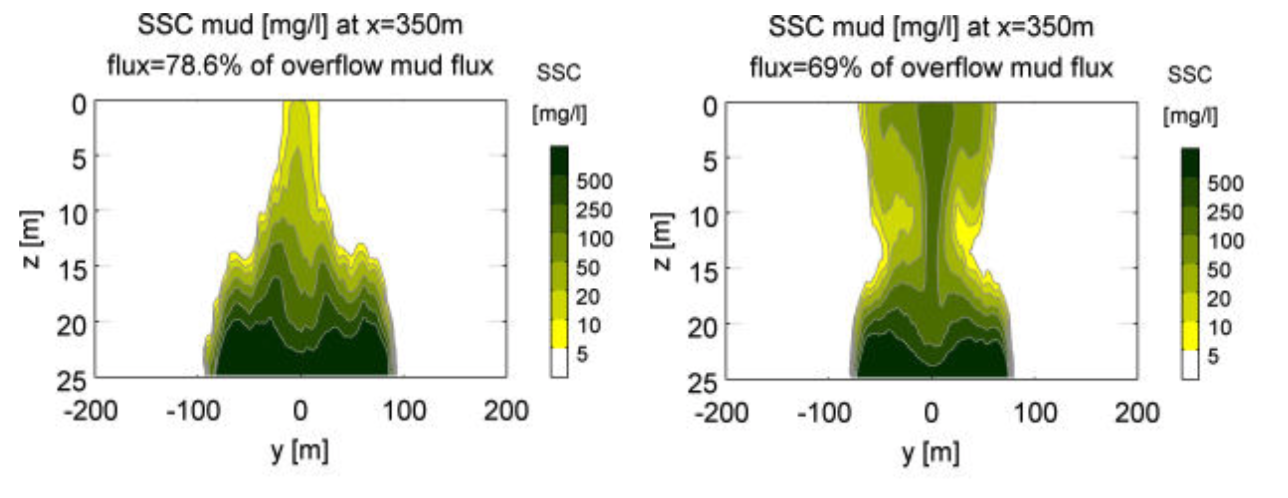
\includegraphics[width = 0.8\textwidth]{Images/air_0_12.png}
    \caption{Simulated result at end near field x =  350m from \cite{Dewit} with left: 0\% air entrainment, right: 12\% air entrainment with $T_p$ = 5.5s}
    \label{fig:air_dewit}
\end{figure}

\noindent The influence of entrained air is conditional, largest influence is found with a low cross flow velocity combined with a large depth. With high cross flow velocity and/or small depth a big surface plume with high turbidity at the free surface can be found, independent of the amount of entrained air \citep{Dewit}. \newline

\noindent \cite{Decrop} tested the effect of the air bubble reduction, by comparing the simulation with- and without air reduction for two cases: a high plume case and a case with plume sediment mixed throughout the water column based on information form \cite{Saremi+}. In figure \ref{fig:air_belg}, the results are shown in terms of vertical sediment concentration profiles at the plume centerline. In the case with deep water and a high plume trajectory (figure \ref{fig:air_belg}a), the effect of decreasing the air entrainment with 90\% is clear. The concentration near the surface is reduced drastically, around a factor 20, which can be explained by the absence of the vertical momentum source in the water-sediment mixture due to the wakes of the rising air bubbles (eq. \ref{eq:bulk}).

\begin{figure}[ht!]
    \centering
    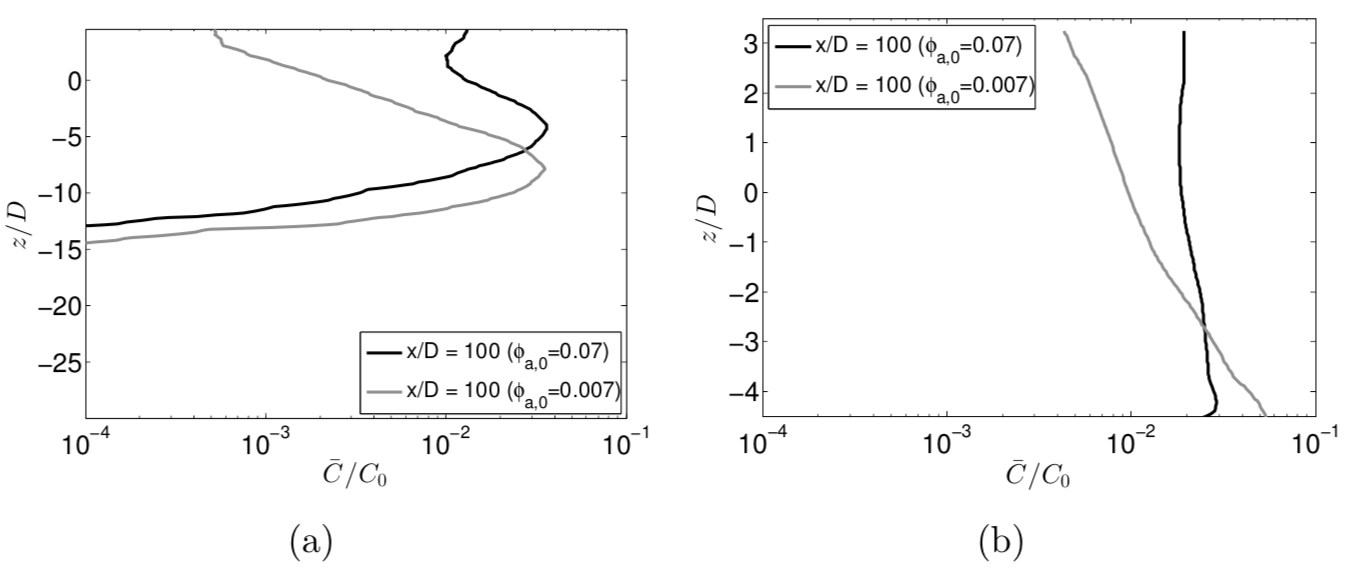
\includegraphics[width = 0.8\textwidth]{Images/air_belg.png}
    \caption{Profiles of time-averaged sediment concentration $C$/$C_0$ for a case with high trajectory (a) and a case with mixed sediments (b). For each case, a simulation is run with a regular initial air bubble volume fraction ($\phi_{a,0}$ = 7\%) and with a 90\% reduction of $\phi_{a,0}$ = 0.7\%}
    \label{fig:air_belg}
\end{figure}

\noindent It is noticed that the bulk of the plume is situated deeper with a reduced air concentration. This effect is simply explained by the increased bulk density of the plume when the air volume fraction is lower. The bulk mass density of the water-sediment-air mixture is defined by:

\begin{equation}
\centering
    \rho_m =  (1-\phi_s-\phi_a)\rho_w + \phi_s\rho_s + \phi_a\rho_a 
    \label{eq:bulk}    
\end{equation}

\noindent where $\phi_s$ and $\phi_a$ are the volume fractions of sediment and air and $\rho_m$, $\rho_s$, $\rho_w$ and $\rho_a$ are the mass densities of respectively the mixture, the sediment, sea water and air. It can be shown that for an air fraction of 7\%, mixtures with $C_0$ up to 13 g/l have a positive buoyancy, which means they are lighter than the surrounding sea water and will flow up to the water surface. For $\phi_a$ = 14\% this is even the case up to $C_0$ = 26 g/l \citep{Decrop}. \newline


\nomenclature[G]{$\rho_a$}{Mass density of air \nomunit{[$kg/m^3$]}}
\nomenclature[G]{$\rho_m$}{Mass density of mixture \nomunit{[$kg/m^3$]}}
\nomenclature[G]{$\phi_s$}{Volume fraction of sediment \nomunit{[-]}}
\nomenclature[G]{$\phi_a$}{Volume fraction of air \nomunit{[-]}}
\nomenclature[G]{$\alpha_y$}{Yaw angle \nomunit{$[^\circ]$}}
\nomenclature[G]{$\psi$}{Angle between the ship centerline and its speed through water \nomunit{$[^\circ]$}}

\noindent In the case with more shallow water and a near-bed density current combined with a surface plume, a different result is found (figure \ref{fig:air_belg}b). The bulk plume volume cannot descend deeper in the case with air reduction, since it is almost fully mixed throughout the water column. The surface concentrations, however, are also positively affected by the air reduction. It can be observed in the figure that with $\psi_{a,0}$ = 7\%, the sediment is mixed, while with $\psi_{a,0}$ = 0.7\%, the surface concentration is about five times lower than the near-bed concentration \citep{Decrop}. As can be seen, the air bubble reduction also has an effect on the plumes in more shallow water, however, it is four times more effective in deep water.













%%%%%%%%%%%%%%%%%%%%%%%%%%%%%%%%%%%%%%%%%%%%%%%%%%%%%%%%%%%%%%%%%%%%%%%%%%%%%%%%%%%%%%%%%%%%%%%%%%%%%%%%%%%%%%%%%%%%%%%%%%%%%%%%%%%%%%%%%%%%%%%%%%%%%%%%


\section{Interaction with propeller}
\label{sec:propeller}
%Belg 8.7.8 + figure 8.3.6
%De wit figuur 7.4

Whether the near-field overflow plume would be different without the propeller jet influence is of course a hypothetical question, no TSHD can sail without propellers. Nevertheless, it is interesting to see how the propeller influences the streamlines around the ship and how this in turn influences the (surface) plume. \newline \noindent Propellers create streamlines extending up- and downstream which show how the propeller jets evolve, see figure \ref{fig:Propeller_belg}. The tangential component of the propeller jet is only short-live: at a distance of 4D (propeller diameter), 90\% has dissipated \citep{Decrop}. 

\begin{figure}[ht!]
    \centering
    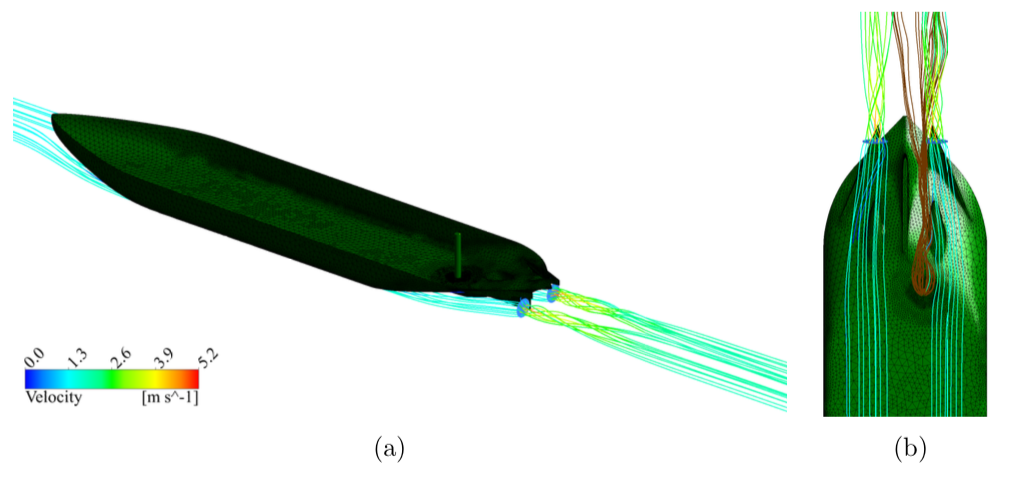
\includegraphics[width = 0.6\textwidth]{Images/Propeller_belg.png}
    \caption{Port side view of the streamlines going through the propellers (a). Bottom view of propeller streamlines and streamlines originating from an overflow with lateral shift of 5m from the centerline(b)}
    \label{fig:Propeller_belg}
\end{figure}

\noindent It can be seen that the propeller jet discharge originates from the keel, but not from the centerline of the keel. In the case of an overflow positioned along centerline of the ship, propeller streamlines do not go directly from overflow to propeller. In case of an overflow shifted from the centerline of the ship (figure \ref{fig:Propeller_belg}b), the sediment might go directly into the propellers.



\noindent The propellers also induce turbulent mixing. Following the gradient diffusion theory, turbulent mixing occurs in down-gradient direction. The vertical turbulent diffusion can be written as

\begin{equation}
    F_z =  -D_t \frac{\delta C}{\delta z}
    \label{eq:turbulent_diffusion}
\end{equation}

\noindent where $D_t$ is the turbulent diffusivity. \newline \newline \noindent
\cite{Decrop} visualized the vertical gradient of C before the plume arrives at the propeller influence. In this case, the propellers are at x/D = 40, but the influence of both propellers arrives at the centerline somewhat further. The propeller jets are located at a height of 0< z/D <3. Two cases can be distinguished: a case with $\delta C$/$\delta z$ <0 before arrival at the propellers and a case with $\delta C$/$\delta z$ >0 at the propeller. \newline 
\noindent In figure \ref{fig:Propeller_belg_2}a, a case is shown with $\delta C$/$\delta z$ <0 before arrival at the propellers (x/D = 30). At x/D = 50 not much influence is found yet. At x/D = 100, however, the effect of the propeller mixing is recognized. The negative vertical concentration gradient is flattened out due to turbulent mixing and thus results in an increase in the surface plume concentration. \newline 

\begin{figure}[ht!]
    \centering
    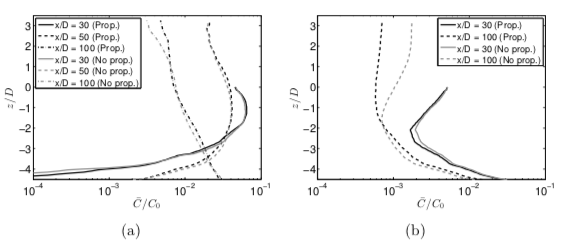
\includegraphics[width = 1\textwidth]{Images/Propeller_belg_2.png}
    \caption{Profiles of time-averaged sediment concentration $C$/$C_0$ for two plume cases: one with $\delta C$/$\delta z$ <0 near the keel and under the stern (a) and one with $\delta C$/$\delta z$ >0 at the same location (b). For each case, a simulation is run with and without propeller jets.}
    \label{fig:Propeller_belg_2}
\end{figure}

\noindent In figure \ref{fig:Propeller_belg_2}b, a case is shown with $\delta C$/$\delta z$ >0. The turbulent sediment flux is here expected to be downward and so the effect of the propeller is positive, particles will be transported downwards. Indeed, at x/D = 100, the sediment in the surface plume seems to be transported by the propeller jets to deeper parts, and the surface plume has a lower concentration. \newline 
\noindent It can be imagined that in most cases, $\delta C$/$\delta z$ might be smaller than zero since the plume emerges from under keel. However, the three-dimensional situation is more complex. The two propeller jets start away from the centerline, widen and meet the centerline after a certain distance. Over the course of this distance, the plume might have risen and $\delta C$/$\delta z$ might be larger than zero. This is again a case of coupled interaction between multiple parameters \citep{Decrop}. \newline

\noindent \cite{Dewit} used his model to look at the influence of a propeller with both normal- and high dredging speed (see figure \ref{fig:Propeller_dewit} for x-direction). It can be seen that a propeller has almost no influence when dredging at high speeds. At normal speeds, the propeller brings the plume up in the vertical. The influence in y-direction can be seen in figure \ref{fig:Overflow_position}. A propeller lifts the dredging plume up by entrainment into the propeller jet an this entrainment partly blocks the counter rotating vortex pair of the dredging plume. However, there is no indication that significant amounts of the dredging plume are sucked in directly into the propeller \citep{Dewit}.

\begin{figure}[ht!]
    \centering
    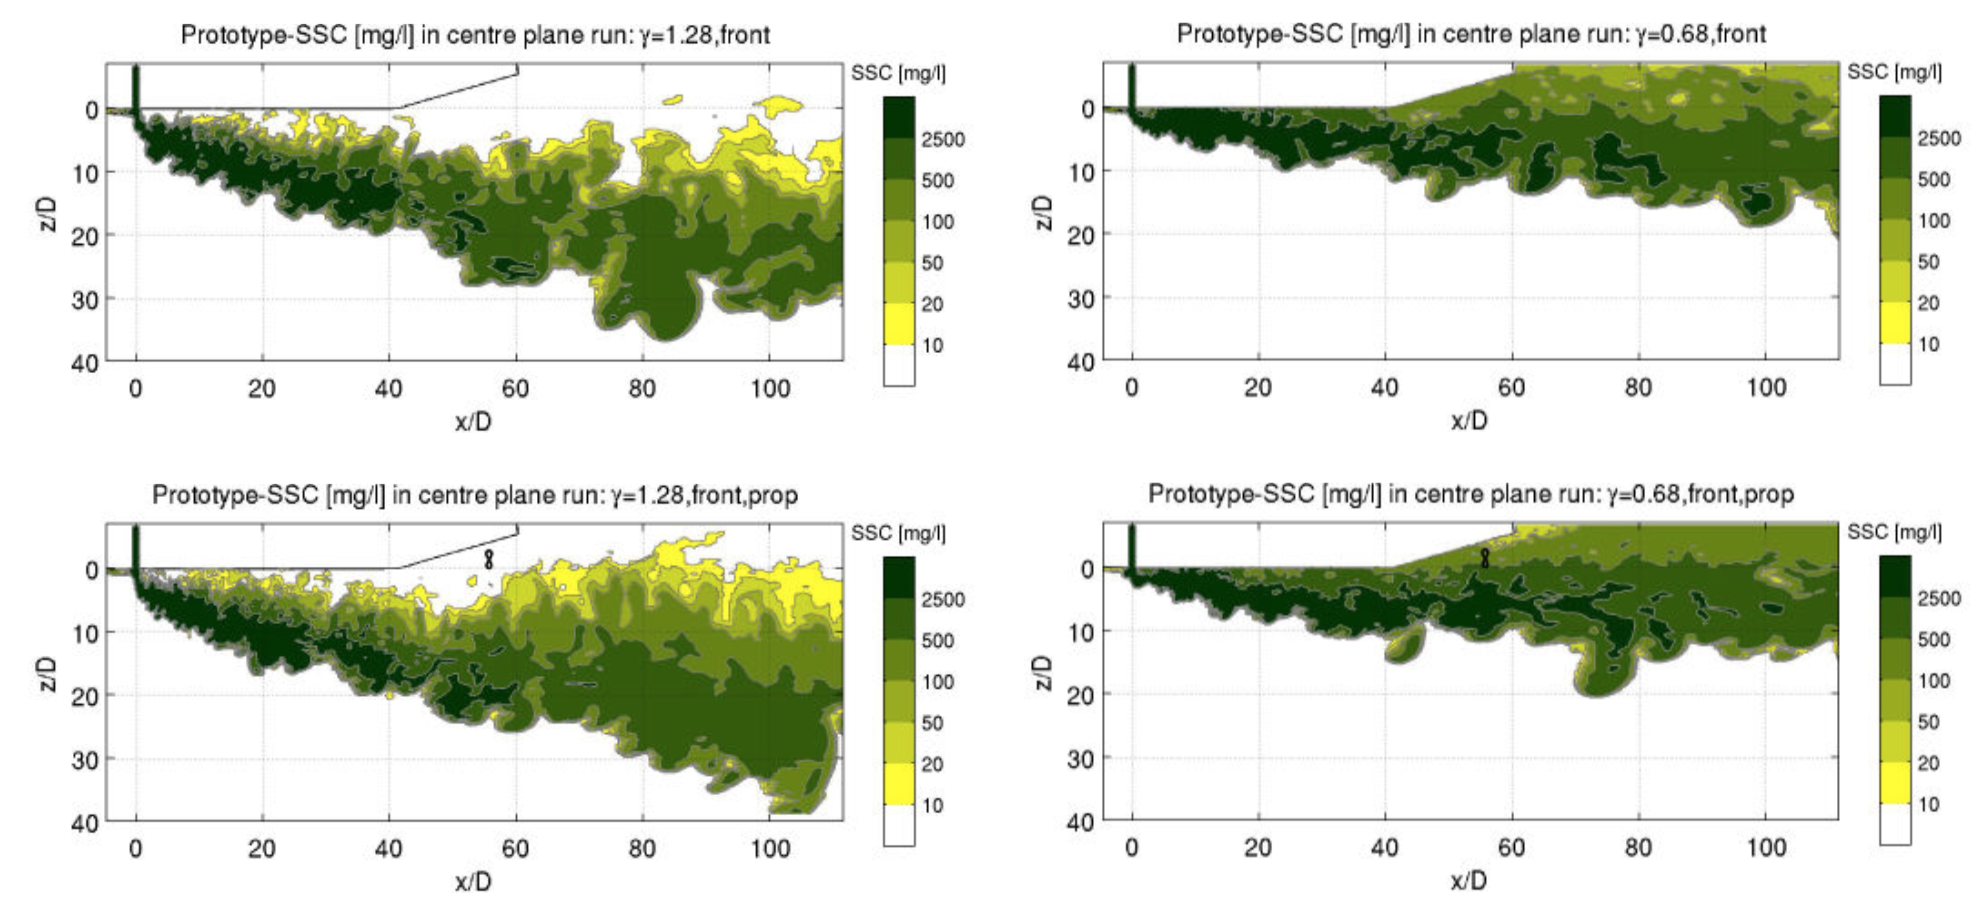
\includegraphics[width = 0.8\textwidth]{Images/Propeller_dewit.png}
    \caption{Influence of propeller with normal dredging speed (left) and high dredging speed (right)}
    \label{fig:Propeller_dewit}
\end{figure}

%







%%%%%%%%%%%%%%%%%%%%%%%%%%%%%%%%%%%%%%%%%%%%%%%%%%%%%%%%%%%%%%%%%%%%%%%%%%%%%%%%%%%%%%%%%%%%%%%%%%%%%%%%%%%%%%%%%%%%%%%%%%%%%%%%%%%%%%%%%%%%%%%%%%%%%%%%%%%%
\newpage
\section{Position of overflow}
\label{sec:position_overflow}
%belg 8.7.9
%De wit (105) + figuur 7.8
%two overflows (belg 8.7.10)

In section \ref{sec:propeller} is was shown that the propeller has influence in the vertical flux distribution of the plume. In addition to this, it can be argued that the distance from the overflow to the propeller could have influence. This will be further discussed in this section. \newline

\noindent Figure \ref{fig:Overflow_position} shows the SSC at x = 100D for normal- and high dredging speed and different locations of the overflow: 22.6D from the front of the TSHD (front) or the overflow at 50.4D from the front of the TSHD (back) \citep{Dewit}. As can be seen, without propeller the plume concentrations do not differ much with the overflow at the front or at the back (figure \ref{fig:Propeller_dewit}). With a propeller the plume has moved upward a little. This effect of the propeller is caused by entrainment into the propeller jet: the dredging plume is sucked upward by this entrainment and fine particles could follow this, depending on particle size diameter, but this is more complex due to hindered settling. When the overflow is at the back, the influence of the propeller is larger, because of the reduced distance between outflow of the dredging plume and the propeller. Figure \ref{fig:Overflow_position2} shows the effect in x direction on the plume of the overflow position. It can be concluded that the position of the overflow and effect of the propellers are in connection with each other. 

\begin{figure}[ht!]
    \centering
    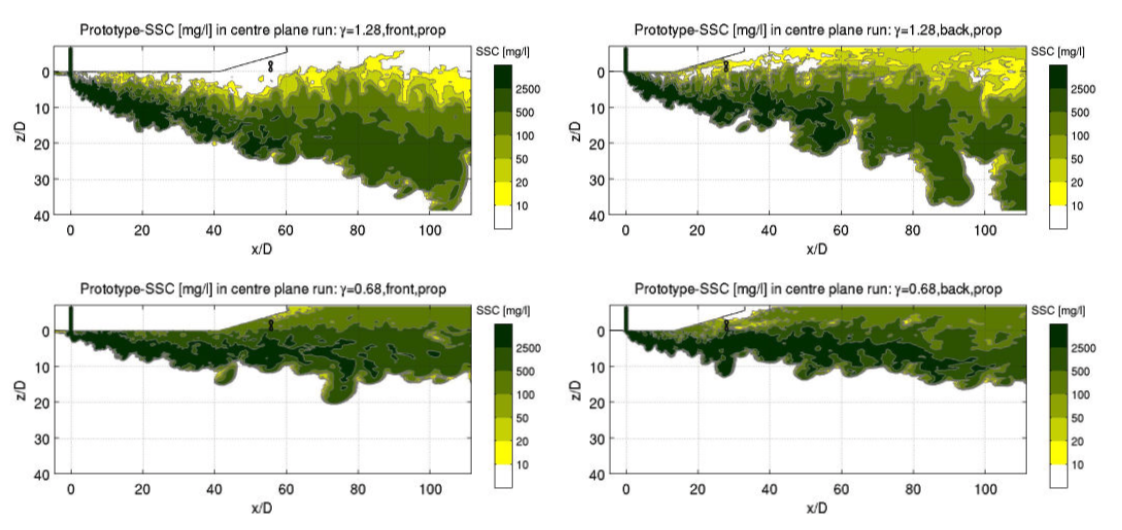
\includegraphics[width = 0.8\textwidth]{Images/Overflow_position_normal_high.png}
    \caption{Simulated instantaneous SSC at the centre slice for runs with normal dredging speed (top) and high dredging speed (bottom) with the overflow position in the front (left) and overflow position on the back (right)}
    \label{fig:Overflow_position2}
\end{figure}



\nomenclature[A]{$L_o$}{Distance from overflow to stern \nomunit{[$m$]}}
\nomenclature[A]{$B_o$}{Lateral distance from overflow to ships centerline \nomunit{[$m$]}}


\begin{figure}[H]
    \centering
    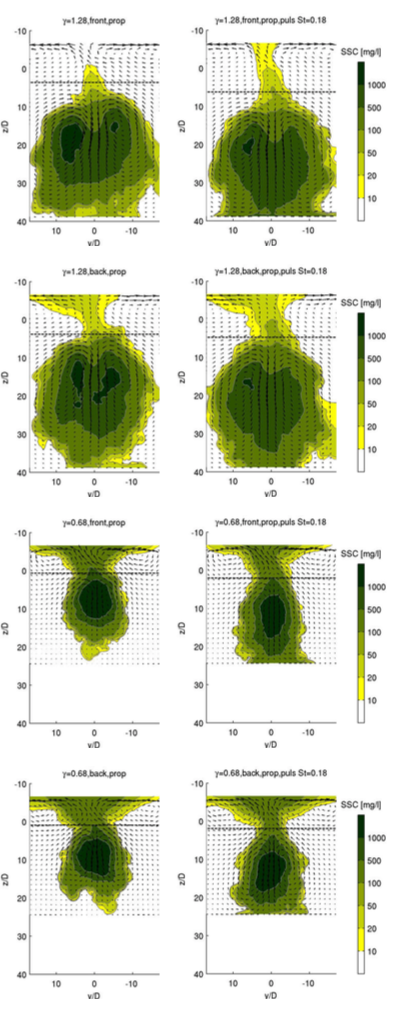
\includegraphics[width = 0.6\textwidth]{Images/Overflow_position.png}
    \caption{Simulated time averaged SSC at x =  100D of different runs with normal and high dredging speed. Arrows indicate the time averaged v, w velocity}
    \label{fig:Overflow_position}
\end{figure}

\noindent \cite{Decrop} used his LES model for the same investigation, however took the position of the overflow relative to the stern with the longitudinal distance between the overflow and stern ($L_o$) and lateral distance ($B_o$) to the ships centerline, which is shown in figure \ref{fig:Overflow_location}. Both the influence of $L_o$ and $B_o$ are investigated. In addition, a case with two overflows (one in the front and one in the back) is examined.

\begin{figure}[ht!]
    \centering
    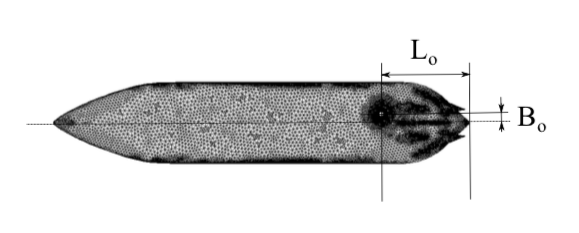
\includegraphics[width = 0.6\textwidth]{Images/Overflow_location_belg.png}
    \caption{Definition of longitudinal- and lateral overflow position $L_o$ and $B_o$}
    \label{fig:Overflow_location}
\end{figure}



\noindent Firstly, the influence of $L_o$ is investigated. It can be assumed that a longer distance $L_o$ is beneficial for the surface plume. When looking at the simulation results of \cite{Decrop} for a relatively horizontal plume (figure \ref{fig:Overflow_position_belg}) the longer distance $L_o$ seems to give the plume more time to detach from the keel and escape the propeller mixing. A smaller $L_o$ (figure \ref{fig:Overflow_position_belg}a) ensures the plume to be caught in the uplifting flow of the propeller and mixes the plume. The result is a much more uniform sediment distribution and a higher concentration in the surface plume.

\begin{figure}[ht!]
    \centering
    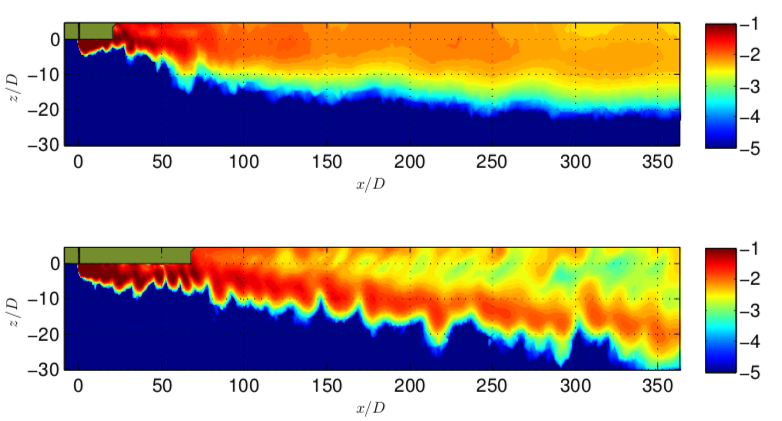
\includegraphics[width = 0.6\textwidth]{Images/Overflow_position_belg.png}
    \caption{Relative sediment concentration log($C$/$C_0$) at the symmetry plane, with H = 40m, $W_0$ = 3.2 m/s, $U_{cf}$ = 1.5 m/s, $C_0$ = 20 g/l and D = 1.1m. Overflow position $L_0$ differs: $L_o$ = 20m (a) and $L_o$ = 80m (b)}
    \label{fig:Overflow_position_belg}
\end{figure}


\noindent When looking at the results for a more dense plume with more rapid descent, the difference between smaller and longer $L_o$ is smaller, see figure \ref{fig:Overflow_position_belg_2}. Already after the short distance $L_o$ = 30m (figure \ref{fig:Overflow_position_belg_2}a), the plume has had the time to detach slightly from the hull. Therefore, the mixing of the propeller jet can just be avoided. The surface plume concentration is therefore only slightly higher compared to the case with $L_o$ = 80 m (figure \ref{fig:Overflow_position_belg_2}b). 

\begin{figure}[H]
    \centering
    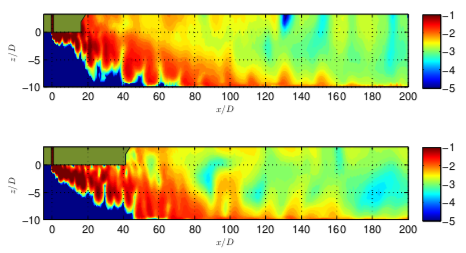
\includegraphics[width = 0.6\textwidth]{Images/Overflow_position_belg_2.png}
    \caption{Relative sediment concentration log($C$/$C_0$) at the symmetry plane, with H = 26 m, $W_0$ = 1.9 m/s, $U_{cf}$ = 2 m/s, $C_0$ = 90 g/l and D = 2 m. Overflow position $L_o$ differs: $L_o$ = 30 m (a) and $L_o$ = 80 m (b)}
    \label{fig:Overflow_position_belg_2}
\end{figure}


\noindent \textbf{Shift in lateral distance} \newline
\noindent In some vessels, an overflow is not located on the centerline of the vessel. The same case as in figure \ref{fig:Overflow_position_belg}a has been simulated with the overflow at $B_o$ = 5m from the centerline (figure \ref{fig:Overflow_position_Bo}). The effect of $B_o$ >0 depends on the geometry of the stern section and of $L_o$. In this case, the strongly curved hull sections near the stern and away from the ship’s centerline cause an uplifting flow, taking the plume upwards and causing an increased surface plume concentration. When the overflow is positioned at the centerline, these sloping parts are not encountered by the plume. At least in the geometry with which this model has been set up \citep{Decrop}.

\begin{figure}[ht!]
    \centering
    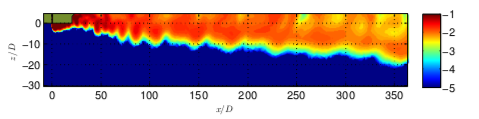
\includegraphics[width = 0.6\textwidth]{Images/Overflow_position_Bo.png}
    \caption{Relative sediment concentration log($C$/$C_0$) at the symmetry plane, boundary conditions same as in figure \ref{fig:Overflow_position_belg}, $L_o$ = 20 m. The lateral overflow position $B_o$ was changed to 5m instead of 0m}
    \label{fig:Overflow_position_Bo}
\end{figure}


\noindent \textbf{Two overflows} \newline
\noindent A case has been set up with the same boundary conditions as in figure \ref{fig:Overflow_position_belg}a. In that figure, two cases are shown. One with $L_o$ = 30m and one with $L_o$ = 80m. In the current case, the overflow discharge has been equally distributed over two overflows by halving the outflow velocity and keeping the same overflow diameter D and concentration $C_0$. The resulting vertical sediment profile at x/D = 100 is shown in figure \ref{fig:Multiple_overflows}. Despite to the lower exit velocity $W_0$, which should be a disadvantage, the plume with multiple overflows has a deeper average position and the overall concentrations are also lower. However, it can be observed (not shown) that due to the lower concentrations in the two overflows, more particles will be in suspension and is more diluted, which will increase the plume width \citep{Decrop}.

\begin{figure}[ht!]
    \centering
    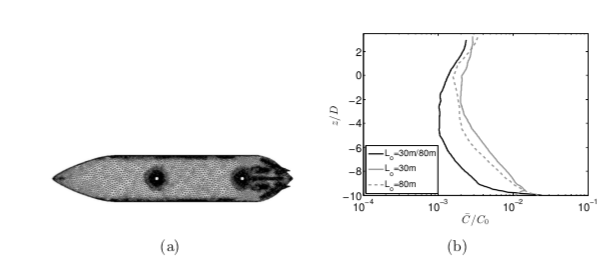
\includegraphics[width = 0.8\textwidth]{Images/Multiple_overflows.png}
    \caption{(a) Top view of the position of the two overflows in the vessel. (b) Profiles of time-averaged sediment concentration $C$/$C_0$ for three plume cases: $L_o$ = 30m/80m with two overflows and two cases with a single overflow at $L_o$ = 30m and 80m}
    \label{fig:Multiple_overflows}
\end{figure}






%%%%%%%%%%%%%%%%%%%%%%%%%%%%%%%%%%%%%%%%%%%%%%%%%%%%%%%%%%%%%%%%%%%%%%%%%%%%%%%%%%%%%%%%%%%%%%%%%%%%%%%%%%%%%%%%%%%%%%%%%%%%%%%%%%%%%%%%%%%%%%%%%%%%%%%%%%%%
\newpage
\section{Overflow sediment load}
%Belg 8.7.5

%Connectie met overflow position belg

The basic dimensionless numbers governing the behaviour of a buoyant jet were identified in section \ref{sec:froudenr} as the densimetric Froude number $F_{\Delta}$ and the velocity ratio $\lambda$. The sediment load in the overflow mixture, $C_0$, influences directly the Froude number $F_{\Delta}$. It is therefore expected that $C_0$ has an influence on the trajectory of near-field dredging plumes. \newline
\noindent \cite{Decrop} compared a total of eight cases with identical water depth H = 16m, $W_0$ = 1.9 m/s, $U_0$ = 1 m/s and D = 2m. The overflow was located at the front end of the hopper, at $L_o$ = 80 m from the stern. The two extremes are shown in figure \ref{fig:Sediment_load}, with $C_0$ = 10 g/l (top) and $C_0$ = 150 g/l (bottom). In these plots, the sediment concentration is shown, as before, as the relative value compared to $C_0$. Since in this case $C_0$ is varied this gives a distorted view. However, it is interesting to see that in the case of $C_0$ = 10 g/l the fraction of the initial sediment discharge ($C_0 Q_0$) present in the surface plume is about 100 times higher compared to the case with $C_0$ = 150 g/l. Evidently, in the field the absolute value of the sediment concentration is of importance. Yet, the question could be raised whether the total amount of sediment brought in suspension during a project could be reduced by releasing a more concentrated mixture. How this could be achieved in practise, is another question.

\begin{figure}[ht!]
    \centering
    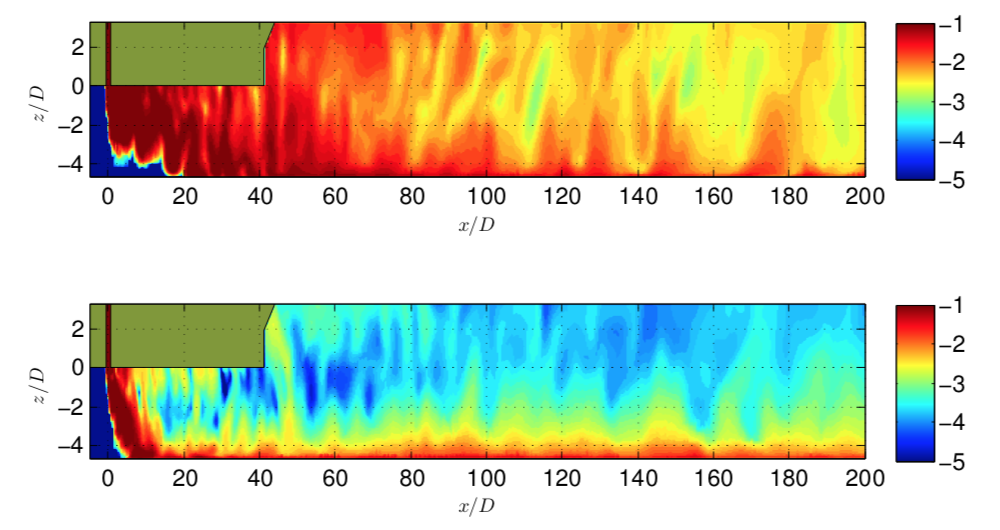
\includegraphics[width = 0.8\textwidth]{Images/Sediment_load.png}
    \caption{Relative sediment concentration log($C$/$C_0$) at the symmetry plane, with H = 16m, $W_0$ = 1.9 m/s, $U_0$ = 1 m/s, $L_o$ = 80m and D = 2m. The sediment concentration at the overflow was varied: $C_0$ = 10 g/l (top) and $C_0$ = 150 g/l (bottom)}
    \label{fig:Sediment_load}
\end{figure}

\noindent Nevertheless, it is needed to analyze the absolute time-averaged concentration C in the surface plume as a function of the release concentration $C_0$. In figure \ref{fig:Sediment_load_2}, the results for simulations with eight different values for $C_0$ are shown by \cite{Decrop}. In this figure, the absolute concentration in g/l is shown at 0.5 m below the water surface. It is surprising to see that very consistently, the sediment concentration in the surface plume decreases when the initial overflow concentration $C_0$ is increased. Between the stern at x/D = 40 and x/D = 120, the surface plume with $C_0$ = 10 g/l has sediment concentrations about twice as high as the plume with $C_0$ = 150 g/l. Further downstream, the difference becomes smaller, to about a factor 1.5. \newline

\begin{figure}[ht!]
    \centering
    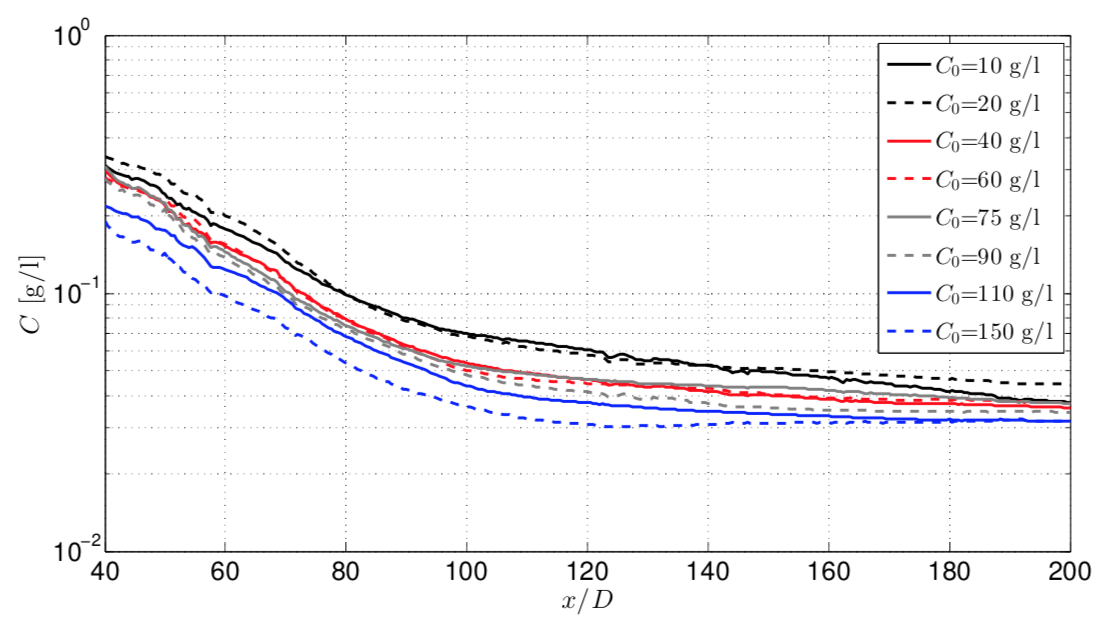
\includegraphics[width = 0.8\textwidth]{Images/Sediment_load_2.png}
    \caption{Comparison of absolute sediment concentration C as function of the initial overflow concentration $C_0$ at z = 0.5m}
    \label{fig:Sediment_load_2}
\end{figure}


\noindent This observation leads to the conclusion that releasing a more concentrated water-sediment mixture could significantly reduce the total amount of sediments brought in suspension.







%%%%%%%%%%%%%%%%%%%%%%%%%%%%%%%%%%%%%%%%%%%%%%%%%%%%%%%%%%%%%%%%%%%%%%%%%%%%%%%%%%%%%%%%%%%%%%%%%%%%%%%%%%%%%%%%%%%%%%%%%%%%%%%%%%%%%%%%%%%%%%%%%%%%%%%%%%%%

\section{Overflow outflow velocity}
%Dewit conclusie

A larger initial overflow velocity brings the overflow plume quicker to the bed, this increases the deposition in the near field and reduces the interaction between the plume and the TSHD hull and the plume and the TSHD propellers. However, an increased overflow velocity also means a larger overflow sediment source flux is brought into suspension \citep{Dewit}. Figure \ref{fig:Overflow_exit_velocity} shows the variation of the overflow exit velocity on $FF_{nf}$ and the vertical distribution (VIF) at x = 350m. It can be concluded that an increase of overflow outflow velocity does not show a large decrease of sediment flux in suspension at the end of the near field.


\begin{figure}[ht!]
    \centering
    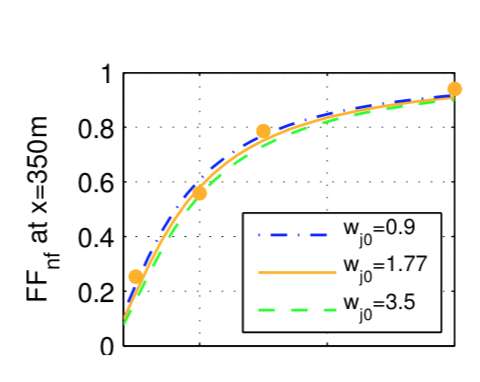
\includegraphics[width = 0.5\textwidth]{Images/Overflow_exit_velocity.png}
    \caption{Influence of overflow exit velocity ($w_{j0}$) at x = 350m}
    \label{fig:Overflow_exit_velocity}
\end{figure}

\noindent \cite{Boot} investigated the near-field spread of an overflow plume in an experimental setting. Three different densities ($\rho$ =  1016, 1033, 1049 $kg/m^3$) and three different outflow velocities ($U_{uitstr}$ =  0.05, 0.1, 0.2 m/s) are used, with a variable ambient flow velocity (6.5, 13 cm/s). With these inputs, \cite{Boot} determined if the outflow stayed a density current, became a transition current or a mixed current (see chapter \ref{sec:plume}) before it hits the bottom of the tank. It is shown, that the outflow velocity and density of the water-sediment mixture are correlated with each other. The increase in density leads to a shift to more density current profile but did not show large differences between the varying velocities with the 6.5 cm/s ambient current. Larger differences are noted when the ambient current increased to 13 cm/s, where all outflow velocities are in the transition zone or mixed flow in exception to $\rho$ =  1049 $kg/m^3$, $U_{uitstr}$ =  0.2 m/s, where it becomes a density current.\newline
\noindent However, in the experimental setup of \cite{Boot} the depth is limited and therefore outcomes can be different with larger depths in practice. Another limitation was the overflow diameter, which was fixed to 2.5cm in the model which should be 5cm to be more exact scaled in practice. In conclusion, the influence of different outflow velocities is limiting, depending on the ambient current. While a density current reaches deeper than a mixed current, it is not concluded in this experiment how deep it reaches compared with the other currents.




\nomenclature[A]{$U_{uitstr}$}{Outflow velocity from experiment by \cite{Boot} \nomunit{$[m/s]$}}


%%%%%%%%%%%%%%%%%%%%%%%%%%%%%%%%%%%%%%%%%%%%%%%%%%%%%%%%%%%%%%%%%%%%%%%%%%%%%%%%%%%%%%%%%%%%%%%%%%%%%%%%%%%%%%%%%%%%%%%%%%%%%%%%%%%%%%%%%%%%%%%%%%%%%%%%%%%%

\section{Overflow shape}
\label{sec:shape}
%Belg (259)

Different studies have shown that non-circular shapes of exit holes of buoyant jets in cross flows have an impact on the jet trajectory. \cite{Salewski+} found that an elliptical jet exit with aspect ratio of 1.69 had a 10\% better penetration in the cross flow compared to a circular hole with the same surface area (at x/D = 10). \cite{Haven+} also showed that high-aspect ratio openings enhance the cross flow penetration. \newline
\noindent These findings lead to the question whether an overflow opening with higher aspect ratio could improve the plume outflow from the TSHD keel wall. \cite{Decrop} simulated  two test cases with a rectangular overflow cross section. The surface area of the rectangular cases was identical to the reference cases with D = 2m shafts. The rectangular shafts were 3m in length (along ship axis) and $\pi$/3m in width. The aspect ratio of the rectangular overflow shaft is therefore equal to $\pi$. All other conditions were kept constant.

\begin{figure}[ht!]
    \centering
    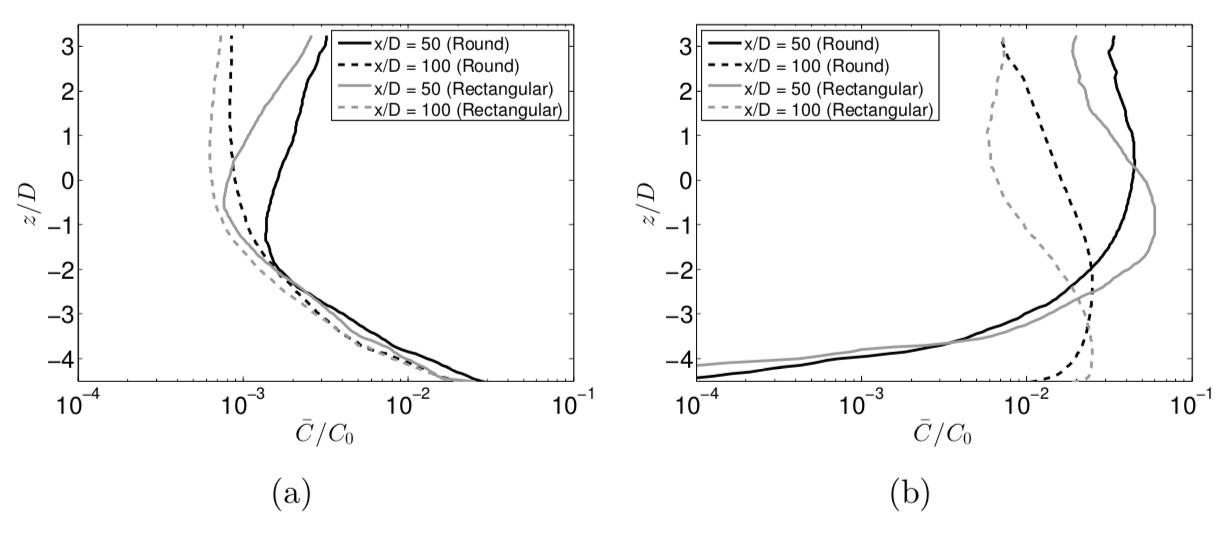
\includegraphics[width = 0.8\textwidth]{Images/Overflow_shape.png}
    \caption{Time-averaged sediment concentration $C/C_0$, for 2 cases in which a round overflow shaft was compared with a rectangular shape with high aspect ratio. For both shapes the cross-sectional area of the overflow shaft was equal to $\pi$. In (a), $U_0$ = 1 m/s, $C_0$ = 55 g/l and $W_0$ = 1.9 m/s. In (b) $U_0$ was increased to 3 m/s}
    \label{fig:Overflow_shape}
\end{figure}

\noindent A first case with $U_0$ = 1 m/s, $C_0$ = 55 g/l and $W_0$ = 1.9 m/s was investigated by \cite{Decrop}(figure \ref{fig:Overflow_shape}a). This case is clearly of type density current with a distinct surface plume. With a round overflow shaft, the sediment concentrations in the upper half of the water column are about 25\% to 50\% higher compared to the case with rectangular overflow. It seems that the shape of the overflow shaft does have an influence in the lower half of the water column. Either the higher aspect ratio in the rectangular case leads to a better escape from the keel, or the more narrow shape of the plume after exit might reduce the number of air bubbles that escape per unit of time, leading to less surface plume generation in the first few meters after the exit.\newline
\noindent In the second case, the cross flow velocity was increased to $U_0$ = 3 m/s. It is determined in this test case whether a high-aspect ratio overflow shaft would lead to a reduction of the surface plume concentration. The result of the simulations of this case with round (D = 2m) and equivalent rectangular shape is shown in figure \ref{fig:Overflow_shape}b. At x/D = 50, it can clearly be observed that the bulk of the plume is situated lower for the rectangular case compared to the round shaft. The surface concentration is 40\% lower in the rectangular case. After x/D = 100, the difference in concentration near the surface has reduced, but it is clear that less sediments are present in the water column in the near-field overflow plume.\newline
\noindent The influence of the shape of the overflow shaft needs more investigation to draw definite conclusions, but it seems that variations in the aspect ratio of the shaft cross section have the potential to reduce the sediments in suspension in the overflow plume. \newline

\noindent In another vision, \cite{Wang} looked at the heat transfer and flow through an elliptic duct and the effect of roundness of the corners with different aspect ratios. The curves are noted with n, which is shown in figure \ref{fig:elliptic_shapes} where c is noted as the aspect ratio (2L is the length of the major axis and 2cL is the length of the minor axis (0 < c $\leq$ 1)). A curve with n=$\infty$ approaches the values of a rectangular duct and a curve with n=$\infty$ and c=1 approaches the values of a square duct.

\begin{figure}[ht!]
    \centering
    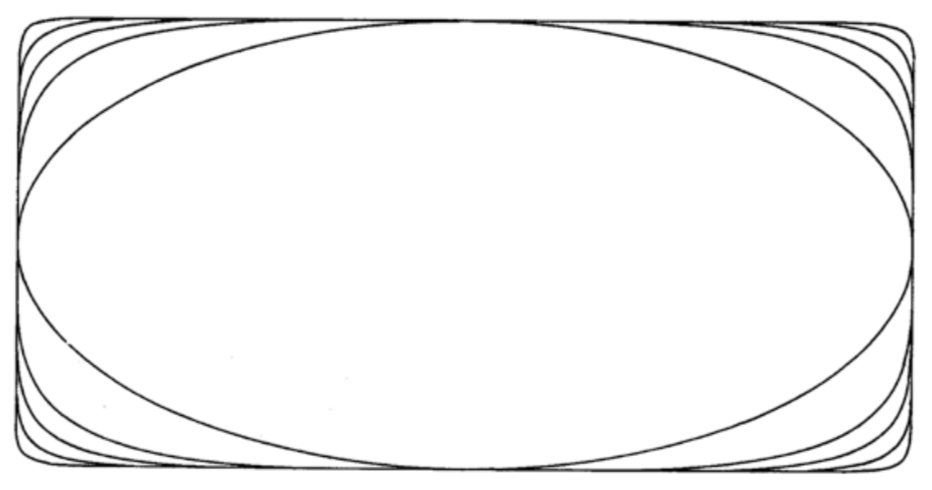
\includegraphics[width=0.5\textwidth]{Images/Elliptic_shapes.png}
    \caption{Super-elliptic cross sections for aspect ratio c = 0.5. Curves from inside: n = 1, 2, 3, 5, 10}
    \label{fig:elliptic_shapes}
\end{figure}

\nomenclature[G]{$\sigma_m$}{Normalized minimum wall shear stress \nomunit{[-]}}
\nomenclature[A]{$c$}{Aspect ratio \nomunit{[-]}}

\noindent The interest of corner rounding is shown by the minimum shear stress ($\sigma_m$) near a rounded corner. As said, with n=$\infty$ the curve approaches the values of a rectangular duct where $\sigma_n$=0 near the corners. The values of $\sigma_n$ with different values of n and c are shown in figure \ref{fig:shapes_table}. Here \cite{Wang} compared different n values with four cases from left to right (c=1, c=0.75, c=0.5, c=0.25).


\begin{figure}[ht!]
    \centering
    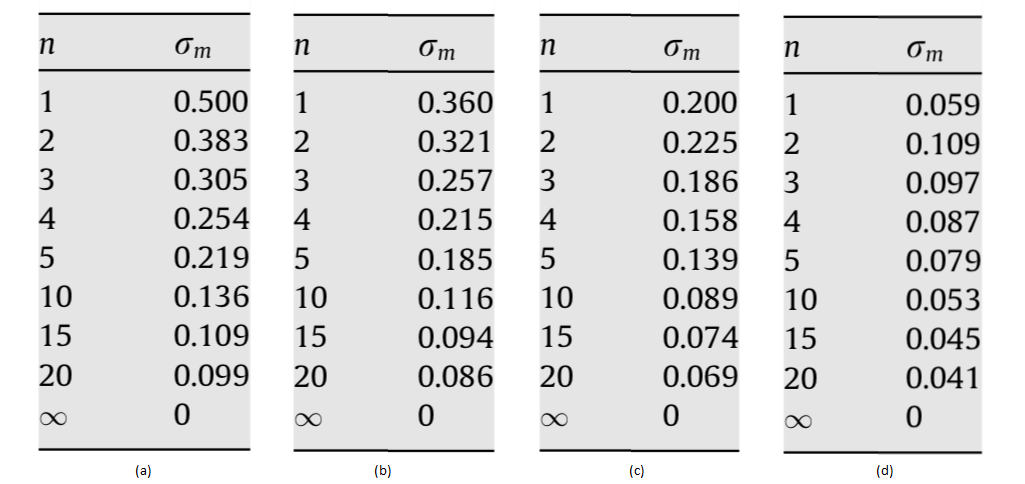
\includegraphics[width=0.8\textwidth]{Images/n_sigma_m.png}
    \caption{Properties of a duct with aspect ratio (a) c=1, (b) c=0.75, (c) c=0.5, (d) c=0.25}
    \label{fig:shapes_table}
\end{figure}


\noindent It is concluded that a rectangular shape with a high aspect ratio (low value of c) shows a decrease in shear stress near the rounded corners ($\sigma_m$) which connects to the founding of \cite{Decrop}.










%%%%%%%%%%%%%%%%%%%%%%%%%%%%%%%%%%%%%%%%%%%%%%%%%%%%%%%%%%%%%%%%%%%%%%%%%%%%%%%%%%%%%%%%%%%%%%%%%%%%%%%%%%%%%%%%%%%%%%%%%%%%%%%%%%%%%%%%%%%%%%%%%%%%%%%%%%%%
\newpage
\section{Extension of overflow}
\label{sec:extension}
%\textbf{Extension of overflow (262) + PHD verslag de wit}

As shown earlier, the water depth and propeller have influence on the plume dispersion while dredging. Both \cite{Dewit} and \cite{Decrop} investigated therefore an extension of the overflow to bring the outflow of the overflow deeper, so bring the sediment closer to the bed, and reduce impact of the propeller. \newline

\noindent \cite{Dewit} investigated three overflow extensions for dredging in a depth of 25m:
\begin{itemize}
    \item Short extension of 3m long
    \item Medium long extension of 8m long
    \item Long extension of 16m long (1m above seabed) 
\end{itemize}

\noindent \cite{Dewit} compared the extensions with a base run (no extension) with following parameters: $\rho_{outflow}$ =  1200 $kg/m^3$, 4 \% air with $T_p$ =  5.5s, $W_0$ =  1.77 m/s, D =  2.25m, depth =  25m, draft =  8m, $\rho_{ambient}$ =  1300 $kg/m^3$. For computational reasons, the overflow shape was square of 2.5m internally. In extension, the 16m overflow was computed to have a horizontal outflow instead of vertical. In order to investigate the interaction between the influence of the THSD sloping aft and propellers, \cite{Dewit} tested two locations: 100m- and 40m in front of the TSHD aft. Figure \ref{fig:Overflow_extension_dewit} shows the suspended sediment concentration for the three overflow extensions.


\begin{figure}[ht!]
    \centering
    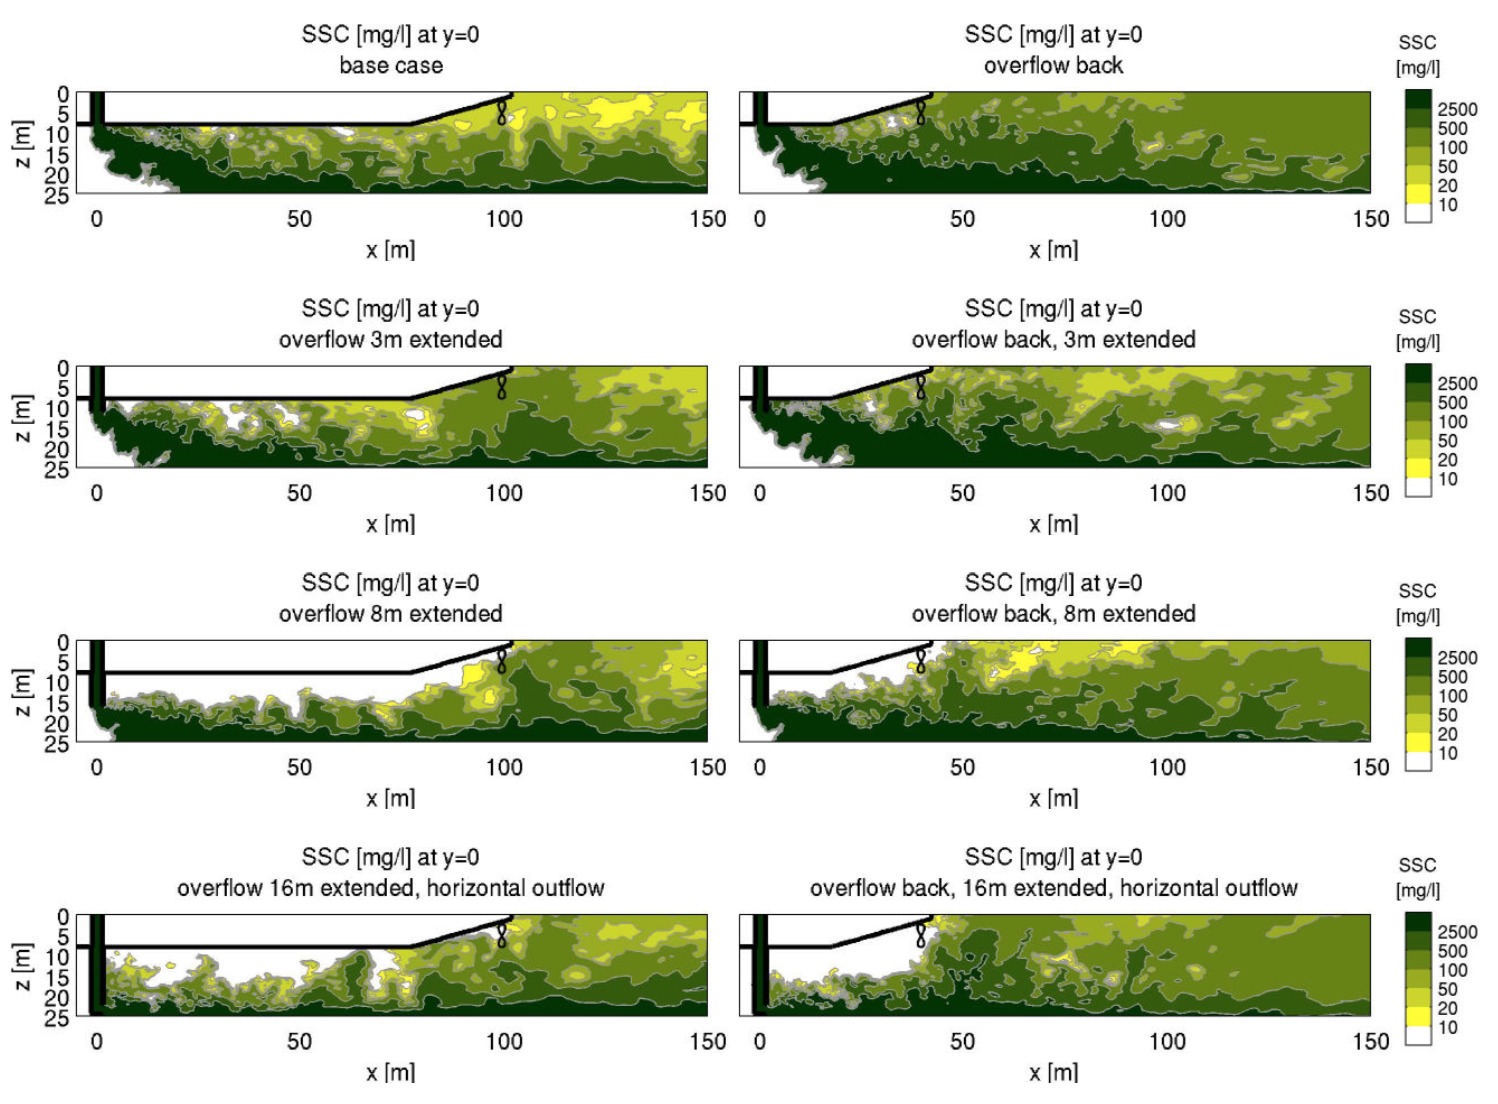
\includegraphics[width = 1\textwidth]{Images/Overflow_extension_dewit.png}
    \caption{SSC at y = 0 for different overflow extensions}
    \label{fig:Overflow_extension_dewit}
\end{figure}

\noindent In the base case, without an overflow extension, the plume spreads over the complete zone below the keel and suspended sediment clouds of SSC > 100 mg/l touch the keel. A 3m extended overflow has limited influence on the instantaneous SSC distribution at y = 0, but a 8m extension results in a zone free of suspended sediment below the keel of the TSHD. The 16m overflow extension brings the sediment right at the bed without mixing, but then the sediment is re-suspended up in the water column by the air fraction from the overflow mixture and the turbulent interaction between the vertical overflow extension and the cross flow. This re-suspension is so strong that some puffs of suspended sediment reach the keel of the TSHD before the sloping aft of the TSHD. The re-suspension caused by air of the 16m overflow extension is larger than the re-suspension by air of the 3m and 8m extensions as the outflow of the 3m and 8m extensions. These two extensions have downward momentum leading to more separation of the air from the sediment-water mixture than with the 16m extension which has horizontal outflow.\newline 
\noindent At the sloping aft, the flow expansion and entrainment into the propeller jet even brings suspended sediment to the free surface. With the overflow at the back the plume spreads more in vertical direction and larger SSC values are found at the free surface than with the overflow at the front. This holds for all cases, with and without overflow extension, and is caused by the shorter distance from the overflow to the TSHD aft and propellers. \newline

\noindent \cite{Decrop} made a case with the LES model to verify the findings of \cite{Dewit}. In addition, the overflow was positioned near the stern of the ship, with a lateral shift of $B_o$ =  4m. In section \ref{sec:position_overflow} it was shown that a lateral shift, and an overflow in the back, were both unfavourable for the creation of surface plumes. \cite{Decrop} compared two overflow extensions (3m, 5m) with a base case with the following parameters: H =  40m, $W_0$ =  3.2 m/s, $U_cf$ =  1.5 m/s, D=1.1m and $C_0$ =  20 g/l. Figure \ref{fig:Overflow_extension_belg} displays the relative sediment concentration at the symmetry plane of $B_0$ =  4m.


\begin{figure}[ht!]
    \centering
    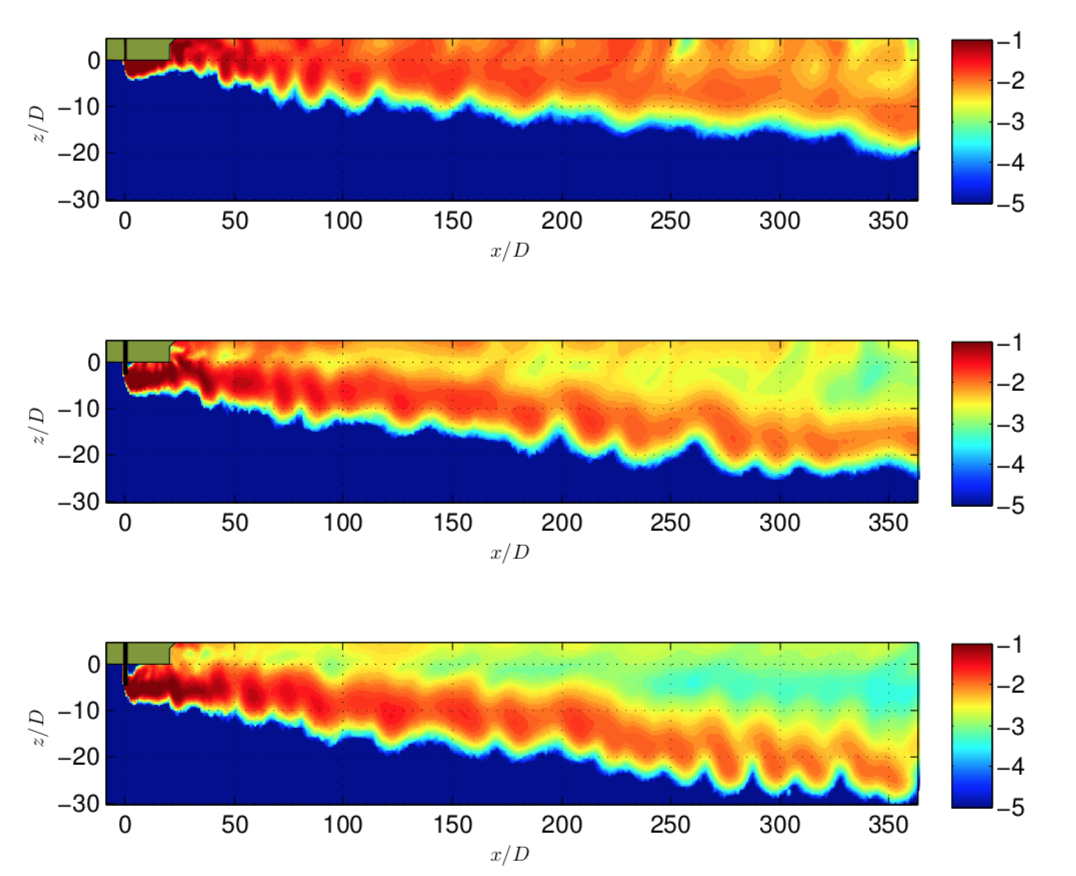
\includegraphics[width = 0.8\textwidth]{Images/Overflow_extension_belg.png}
    \caption{Relative sediment concentration log($C/C_0$) at $B_0$ =  4m with overflow extension =  0m (top), 3m (middle), 5m (bottom)}
    \label{fig:Overflow_extension_belg}
\end{figure}

\noindent It can clearly be observed that in the case with no extension, the overflow plume moves completely to the surface (top panel). With an extension length of 3m, the main plume is allowed to escape the uplifting effect of the curved stern sections, but a relatively high sediment concentration remains present in a surface plume (middle panel). This can be explained by the fact that the plume was not deep enough to escape the propeller jet. For an extension length of 5m, the plume escapes both the uplifting of the stern and the propeller jet mixing (bottom panel). The main plume descends steadily towards the sea bed. Air bubbles still have an influence, which cannot be avoided unless an over
overflow extension is combined, for example, with an environmental valve. However, it is noted that an environmental valve is inefficient with an lateral shift of the overflow \citep{Decrop}. It can be seen that even in the case with an overflow length of 5m, some sediment is torn off above the plume right after the exit, due to air bubble entrainment. \newline

\noindent Additionally, \cite{Decrop} made an overview of the vertical $C/C_0$ profiles (figure \ref{fig:Overflow_extension_belg_2}) for different extension lengths and two distances behind the dredger.


\begin{figure}[ht!]
    \centering
    \includegraphics[width = 1\textwidth]{Images/Overflow_extension_belg_2.png}
    \caption{Vertical profiles of time-averaged sediment concentration $C/C_0$}
    \label{fig:Overflow_extension_belg_2}
\end{figure}

\noindent Figure \ref{fig:Overflow_extension_belg_2}a shows the profiles at x/D=100. It can be observed that the maximum concentration in the plumes remains similar, but that the plume center is deeper for longer extension lengths. The difference between the depth of the concentration (at $10^{-4}$ in figure \ref{fig:Overflow_extension_belg_2}), for extension lengths 3m and 5m is larger then the difference in extension length (2m). More important is the fact that the surface concentration decreases a factor 2.5 with a 3m extension and a factor 5 with a 5m extension. When looking further downstream (x/D=300; figure \ref{fig:Overflow_extension_belg_2}b), the same pattern is found, where plumes with increasing extension are deeper and have a lower surface concentration. The surface plume reductions at x/D=300 are smaller, but still noticeable. \newline

\noindent The extension, as showed, has noticeable positive effects on the surface plume. However, an overflow extension will create a extra torque around the point where the extension is connected to the hull. In addition, the extended overflow pipe will have strong interaction with the ambient flow, which creates a different flow pattern. 







%%%%%%%%%%%%%%%%%%%%%%%%%%%%%%%%%%%%%%%%%%%%%%%%%%%%%%%%%%%%%%%%%%%%%%%%%%%%%%%%%%%%%%%%%%%%%%%%%%%%%%%%%%%%%%%%%%%%%%%%%%%%%%%%%%%%%%%%%%%%%%%%%%%%%%%%%%%%
%TABEL MET OPSOMMING VAN ELKE FACTOR VOOR EN NADELEN ETC.
%grootste factoren volgens belg en de wit
%MCA en keuze welke factor aanpakken

\newpage
\section{Conclusion}
\nomenclature[Z]{MCA}{Multi Criteria Analysis}


In the past paragraphs, twelve factors are investigated to decrease the surface turbidity of overflow losses on a TSHD. In order to get a good overview, which factors are the most promising to investigate further into an practical solution, the factors are divided in three parts: A recommendation- , no influence- or a further investigation part. A multi-criteria-analysis is done to conclude which factor is the most promising solvable factor that will be further investigated into a practical solution. In this MCA questions like, is a solution practical possible? or is it economic feasible? will be answered. First all factors are showed in an overview (Table \ref{tab:Overview_factors}) with a short conclusion. \newline 

\begin{table}[ht!]
\centering
\caption{Overview contributing factors which lead to surface turbidity , with their conclusions}
\label{tab:Overview_factors}
\begin{adjustbox}{max width=\textwidth}
\begin{tabular}{|l|l|}
\hline
\textbf{Factor}                        & \textbf{Conclusion}                                                                                                                                                                                                                                                                                                                                                                   \\ \hline
Hopper inlet / sedimentation           & Change the filling process to decrease overflow losses in the last phase, where these increase exponentially                                                                                                                                                                                                                                                            \\ \hline
Dredging speed                         & \begin{tabular}[c]{@{}l@{}}An increase of $U_{cf}$ of 3, will increase the surface plume concentration $C/C_0$ 10 times at X/D = 100 \\ Horizontal spreading is decreased with a higher dreding speed\end{tabular}                                                                                                                                                                    \\ \hline
Dredging / water depth                 & \begin{tabular}[c]{@{}l@{}}A keel clearance of \textgreater 9m will not decrease the surface plume concentration more\\ An increase from $H_k$ = 5m to $H_k$ = 9m increases the surface streamwise velocity around a factor 1.3\\ An increase of water depth will increase the amount of flux near the bed\end{tabular}                                                               \\ \hline
Angle between TSHD \& ambient current & \begin{tabular}[c]{@{}l@{}}Due to the angle, surface plume is diverted\\ Total sediment flux is quite similar compared without cross flow \\ More interaction with hull and propeller, leads to upward flow to surface\end{tabular}                                                                                                                                                                                                                                \\ \hline
Pulsing                                & \begin{tabular}[c]{@{}l@{}}Pulsing correlated with air entrainment, increase in pulsing will increase air entrainment\\ Increase in pulsing period ($T_p$) will increase surface plume\\ Pulsing period does not have large effect with a high dredging speed\end{tabular}                                                                                                            \\ \hline
Air                                    & \begin{tabular}[c]{@{}l@{}}Entrained air will follow a other path than the water-sediment mixture\\ Air will release to the surface after outflow of the overflow and could take fine particles with it\\ 12\% air with $T_p$ = 5.5s will increase the surface plume concentration with 200 mg/l and\\ spreads the surface plume with 100m compared to case with 0\%\end{tabular}     \\ \hline
Interaction with propeller             & \begin{tabular}[c]{@{}l@{}}Tangential component of propeller is 90\% dissipated at 4D\\ Almost no influence at high dredging speed\\ Lifts the plume from 20 mg/l (no propeller) to 50 mg/l at normal dreding speed at propeller height\\ A propeller was found to have more influence than overflow location and pulsing on the formation of a \\surface plume\end{tabular}                                                                                                                                  \\ \hline
Position of overflow                   & \begin{tabular}[c]{@{}l@{}}Position in the front of TSHD will decrease surface plume\\ Correlated with propeller, more is sucked in if overflow is at the back\\ Lateral shift of overflow will increase the surface plume\\ Multiple overflows (front and back) has deeper average position of plume and overall concentrations are \\ lower, plume width will increase\end{tabular} \\ \hline
Overflow sediment load                 & \begin{tabular}[c]{@{}l@{}}Absolute sediment concentrations will decrease with a factor 2 near the TSHD (40 \textless x/D \textless 120) and with \\ a factor 1.5 when increasing the overflow sediment load from $C_0$ = 10 g/l to $C_0$ = 150 g/l\\ from x/D \textgreater 120 when increasing the overflow sediment load from $C_0$ = 10 g/l to $C_0$ = 150 g/l\end{tabular}        \\ \hline
Overflow outflow velocity              & Overflow outflow velocity does not show a large decrease of sediment flux in suspension at end of near field                                                                                                                                                                                                                                                                          \\ \hline
Overflow shape                         & \begin{tabular}[c]{@{}l@{}}Rectangular shape will decrease sediment concentration in upper water column with 25-50\% in normal speed\\ Rectangular shape will decrease sediment concentration in upper water column with 40\% in high speed with\\ aspect ratio of $\pi$\end{tabular}                                                                      \\ \hline
Extension of overflow                  & \begin{tabular}[c]{@{}l@{}}Extension of overflow will bring plume deeper, but creates more re-suspesion because of air\\ Surface concentration decreases with factor 2.5 with 3m extension\\ Surface concentration decreases with factor 5 with 5m extension\end{tabular}                                                                                                             \\ \hline
\end{tabular}
\end{adjustbox}
\end{table}


\noindent Directly, the twelve factors can be divided in divided in three parts, where one part are more recommendations, other need further investigation to determine the amount of surface plume created and the last concluded to have more or less no influence on the creation of a surface plume. A good example is the dredging speed, which will be recommended to keep low. Table \ref{tab:Overview_factors} showed a 10 times increase in surface plum if the dredging speed is increased with a factor 3. The twelve factors are divided in these two parts and are shown in table \ref{tab:Part_factors}. In addition, all factors are described further why they are placed in a certain group.



\begin{table}[ht!]
\centering
\caption{Overview of splitting all factors in three parts: recommendation, no influence or further investigation}
\label{tab:Part_factors}
\begin{tabular}{|l|l|l|}
\hline
\textbf{Recommendations}              & \textbf{No Influence}      & \textbf{Further Investigation} \\ \hline
Dredging / water depth                & Overflow outflow velocity  & Hopper inlet / sedimentation   \\ \hline
Dredging speed                        & Interaction with propeller & Pulsing / Air                  \\ \hline
Position of overflow                  &                            & Overflow sediment load         \\ \hline
Angle between TSHD \& ambient current &                            & Overflow shape                 \\ \hline
                                      &                            & Overflow extension             \\ \hline
\end{tabular}
\end{table}



\newpage
\begin{itemize}
    \item \textbf{Hopper inlet / sedimentation} [\textit{Further investigation}]: The amount of surface plume is directly related to the amount of concentration in the overflow. A way to decrease the overflow loss in the hopper must be further investigated.
    \item \textbf{Dredging speed} [\textit{Recommendation}]: It is recommended that the dredging speed stays at normal level. Increase to higher dredging speed will exponentially increase the surface plume.
    \item \textbf{Dredging / water depth} [\textit{Recommendation}]: It is recommended that the water depth is larger than 9m. A water depth <9m will increase the surface plume and streamwise velocity. 
    \item \textbf{Angle between TSHD \& ambient current} [\textit{Recommendation}]: The total sediment flux is quite similar compared without a cross flow, only the plume is diverted. However, interaction with hull can be expected with higher angles, where sediment particles can be taken along by the expanding flow towards the free surface. Recommended to keep angle between TSHD and ambient current low.
    \item \textbf{Air / pulsing} [\textit{Further investigation}]: Air and pulsing are closely correlated because pulsing causes the inlet of air in the overflow. A solution which decreases the amount of entrapped air or pulsing must be investigated further.
    \item \textbf{Interaction with propeller} [\textit{No influence}]: A propeller does have influence on the surface plume due to the suction force by the propeller. However, a TSHD needs a propeller and therefore this is not further investigated.
    \item \textbf{Position of overflow} [\textit{Recommendation}]: A overflow that is positioned in the front of the TSHD will decrease surface plume because less interaction with the propeller. In addition, two overflows (front and back) will bring plume deeper.
    \item \textbf{Overflow sediment load} [\textit{Further investigation}]: Absolute sediment concentration will decrease with factor 2 near TSHD and with a factor 1.5 further away when increasing the overflow sediment load from $C_0$ = 10 g/l to $C_0$ = 150 g/l. Further investigation is needed to show if it is practical possible.
    \item \textbf{Overflow outflow velocity} [\textit{No influence}]: A change in overflow outflow velocity did not show a large decrease of sediment flux in suspension, so it is not further investigated.
    \item \textbf{Overflow shape} [\textit{Further investigation}]: A rectangular overflow shape showed a strong decrease of surface plume and so must be further investigated.
    \item \textbf{Overflow extension} [\textit{Further investigation}]: A overflow extension of >3m showed a strong amount of decrease in surface concentration and so must be further investigated.
\end{itemize} 


%Alle grafiek waardes weten!!! Decrop deWit

%milieu eisen dredging Australie bijvoorbeeld 

%korrelgrootte




\chapter{Description Investigated Solutions}

\noindent The factors which need further investigation are now compared in a MCA to see which factor is most promising to create a practical solution for. Firstly, a short description of solutions for each factor is presented. Designs that decrease turbidity and that are currently available are shown in Appendix \ref{app:current_designs}.


\newpage
\section{Short description possible solutions}

\textbf{Hopper inlet / sedimentation} \newline
\noindent As said earlier, the best way to decrease surface turbidity theoretically is to let no sediment into the overflow at all. Therefore a solution could be some kind of centrifugal filter setup to filter the sediment and water, where the water can leave the overflow. Instead of the water sediment mixture flows in the overflow, it is sucked up by a pump where it is filtered and the sand can be stored on the TSHD. Therefore no sediment will flow out of the overflow and there will be only a plume caused by the dredge head. Theoretically it is the desirable solution, however, extra room has to be created for the filter setup which can cause practical problems.  \newline

\noindent \textbf{Air / Pulsing} \newline
\noindent Solutions for the intake of air are available which are further explained in appendix \ref{app:current_designs}. However, especially the the green valve has a big disadvantage about the controls during operation which are vulnerable for the sediment in the overflow. Therefore, a simplistic design is preferred which will reduce the pulsing and so the entrapped air into the overflow. \newline A possible solution is (1) a floating overflow, so that the overflow always fills from underwater and no air can be entrapped. In this case, a floating overflow headpiece is placed on a shaft which will increase in height if the hopper is filled. Around the shaft, openings are placed where the water sediment mixture can flow in and due to the rising of the floating overflow headpiece, the openings are only placed underwater so no air can flow into the overflow. This option is however only possible when replacing the whole overflow. Therefore another option is (2) a filter that will stop / reduce air inflow, which is placed on the current overflow inlet piece. \newline

\noindent \textbf{Overflow sediment load} \newline
\noindent Increasing the sediment load in the overflow showed a great decrease of sediment in suspension. This can be achieved by either (1) block the sediment (where water can pass) and release it all together due to a kind of filter layer or (2) inject extra sediment particles to increase the sediment load in the overflow. In this case nozzles are placed in the overflow which will inject extra particles so that the concentration can increase and kept constant. A drawback to this solution is the extra added parts that will need maintenance and are vulnerable to faults during operation.\newline

\noindent \textbf{Overflow shape} \newline
\noindent Different shapes can be tested to see which shape decreases the surface turbidity the most. Additionally, a practical solution to add to current TSHD's overflow should be considered. \newline (1) Change the overflow shape by adding a diffusor that changes shape or (2) mold the best shape in the current overflow system. \newline

\noindent \textbf{Overflow extension} \newline
\noindent As shown, an overflow extension is a good solution to decrease the surface turbidity. However a practical solution is a little bit harder. The extension creates a different flow underwater and must resist the force in the water. Also the connection to the hull, to make the extension a good solution for current TSHD's, should be investigated. \newline Therefore two cases can be considered: (1) an overflow extension that is connected to the hull which can be lifted up by some mechanism. This could be made from either stainless steel, which cannot bend, or a rubberized material so that it could bend with the current to decrease the force on the extension. However, the material should withstand the bending and fatigue which needs further investigation. A second option is (2) an extension which let the sediment flow out at the dredge head. In this case a connection can be made from the overflow outflow to the dredge head so that the sediment leaves the new overflow near bed level. However, in this case, as shown in section \ref{sec:extension}, the re-suspension is so strong that some suspended material reach the keel of the vessel.






%Luchtfilter

%Overflow verlengen (makkelijke bevestiging (klapmechanisme), duurzaam materiaal, niet te hoge kracht (rubberring pa?)  -> Overflow naar zuigbuis

%Iets toevoegen zodat density in overflow verhoogd wordt waardoor materiaal makkelijker en sneller zinkt (zandfilter of iets dergelijks?)

%Shape overflow, verschillende vormen testen

%Siphon idee
%livingstone standpipe idee (zie http://www.hobbykwekers.nl/artikelen/item/6-manieren-van-overlopen)

%Drijvende overflow







%%%%%%%%%%%%%%%%%%%%%%%%%%%%%%%%%%%%%%%%%%%%%%%%%%%%%%%%%%%%%%%%%%%%%%%%%%%%%%%%%%%%%%%%%%%%%%%%%%%%%%%%%%%%%%%%%%%%%%%%%%%%%%%%%%%%%%%%%%%%%%%%%%%%%%%%%%%%

\section{Analysis for further investigation of practical solution}

The proposed solutions are further investigated in a multi criteria analysis. In this analysis, all solutions are compared with each other in a certain amount of factors and each factor is given a weight factor for importance. The MCA is shown in table \ref{tab:MCA}, but first each factor is further elaborated what the meaning is.  \newline

\noindent \textbf{Practicality}\newline
Smaller implementations are more practical than bigger ones. Does the implementation of the solution change the working method of the TSHD or negatively influence the working on a TSHD for the people and the ease of installation of the solution can be noted for this factor. Also a distinction can be made between an active- and passive solution where an active system has moving parts or must be powered where a passive solution doesn't. A good solution can have great efficiency, but also needs practical appliance. Therefore the practicality has a weight factor of 0.25.\newline

\noindent \textbf{Economics} \newline
Another important factor is the total cost of the solution. What will be the cost for the production of the solution and what is the expected lifetime of the product before it has to be replaced are questions that can be asked for this factor. The economics are estimated based on complexity, material and size. To keep a good view at the budget needed for a solution, the economics has a weight factor of 0.2.\newline

\noindent \textbf{Theoretical efficiency}\newline
The theoretical efficiency is obviously relevant for a solution to decrease the surface turbidity. Here, all solutions are elaborated purely based on theoretical efficiency, which was investigated in chapter \ref{CH:influence_factors}. If it is not clear exactly how much the surface turbidity / flux in suspension is decreased, an estimate is based on information of chapter \ref{CH:influence_factors}. As the main drive is to decrease the surface turbidity / sediment in suspension, the theoretical efficiency is weighted highest with a weight factor of 0.3.\newline

\noindent \textbf{Maintainability}\newline
The ease to maintain all solution is clarified here. Some solutions are bigger and have moving parts which need to maintained more often. The ease to reach to the parts which need to be maintained could also be noted. As stated before, the maintainability is important and therefore has a weight factor of 0.15. \newline

\noindent \textbf{Adjustment to TSHD}\newline
Is the solution simple implemented on a TSHD, does the TSHD need some adjustments before implementation, or is it a solution for newly build vessels. As this is not clearly stated in the thesis proposal, this factor is weighted lowest with a factor 0.1. \newline

\noindent \textbf{Test possibility} \newline
How easy can the possibilities be tested in the experimental setups present at APT Offshore or TU Delft. \newline

\noindent All solutions are ranked from 1 to 5, where 5 is ranked as best for that factor and 1 for the worst. As there are 9 solutions, factors can have the same ranked value. 

%\caption{Multi Criteria Analysis with weight factors to determine most promising solution}
%\label{tab:MCA}
%\begin{adjustbox}{max width=\textwidth}
%\end{adjustbox}


\begin{table}[ht]
\centering
\caption{Multi Criteria Analysis with weight factors to determine most promising solution}
\label{tab:MCA}
\begin{adjustbox}{max width=\textwidth}
\begin{tabular}{lcccccccc}
\cline{1-7} \cline{9-9}
\multicolumn{1}{|c|}{\textbf{Solution}}       & \multicolumn{1}{c|}{\textbf{Practicality}} & \multicolumn{1}{c|}{\textbf{Economics}} & \multicolumn{1}{c|}{\textbf{Theoretical efficiency}} & \multicolumn{1}{c|}{\textbf{Maintainability}} & \multicolumn{1}{c|}{\textbf{Adjusment to TSHD}} & \multicolumn{1}{c|}{\textbf{Test possibility}} & \multicolumn{1}{c|}{\textbf{}} & \multicolumn{1}{c|}{\textbf{Total}} \\ \cline{1-7} \cline{9-9} 
\multicolumn{1}{|l|}{Sediment filter on TSHD} & \multicolumn{1}{c|}{3}                     & \multicolumn{1}{c|}{1}                  & \multicolumn{1}{c|}{5}                               & \multicolumn{1}{c|}{2}                        & \multicolumn{1}{c|}{2}                          & \multicolumn{1}{c|}{2}                         & \multicolumn{1}{c|}{}          & \multicolumn{1}{c|}{2,85}           \\ \cline{1-7} \cline{9-9} 
\multicolumn{1}{|l|}{Floating overflow}       & \multicolumn{1}{c|}{3}                     & \multicolumn{1}{c|}{2}                  & \multicolumn{1}{c|}{3}                               & \multicolumn{1}{c|}{3}                        & \multicolumn{1}{c|}{1}                          & \multicolumn{1}{c|}{1}                         & \multicolumn{1}{c|}{}          & \multicolumn{1}{c|}{2,35}           \\ \cline{1-7} \cline{9-9} 
\multicolumn{1}{|l|}{Air filter insert}       & \multicolumn{1}{c|}{5}                     & \multicolumn{1}{c|}{4}                  & \multicolumn{1}{c|}{4}                               & \multicolumn{1}{c|}{4}                        & \multicolumn{1}{c|}{5}                          & \multicolumn{1}{c|}{1}                         & \multicolumn{1}{c|}{}          & \multicolumn{1}{c|}{3,90}           \\ \cline{1-7} \cline{9-9} 
\multicolumn{1}{|l|}{Blockage filter}         & \multicolumn{1}{c|}{2}                     & \multicolumn{1}{c|}{4}                  & \multicolumn{1}{c|}{4}                               & \multicolumn{1}{c|}{4}                        & \multicolumn{1}{c|}{4}                          & \multicolumn{1}{c|}{2}                         & \multicolumn{1}{c|}{}          & \multicolumn{1}{c|}{3,20}           \\ \cline{1-7} \cline{9-9} 
\multicolumn{1}{|l|}{Inject extra sediment}   & \multicolumn{1}{c|}{3}                     & \multicolumn{1}{c|}{3}                  & \multicolumn{1}{c|}{4}                               & \multicolumn{1}{c|}{2}                        & \multicolumn{1}{c|}{3}                          & \multicolumn{1}{c|}{3}                         & \multicolumn{1}{c|}{}          & \multicolumn{1}{c|}{3,15}           \\ \cline{1-7} \cline{9-9} 
\multicolumn{1}{|l|}{Diffusor}                & \multicolumn{1}{c|}{4}                     & \multicolumn{1}{c|}{5}                  & \multicolumn{1}{c|}{3}                               & \multicolumn{1}{c|}{4}                        & \multicolumn{1}{c|}{4}                          & \multicolumn{1}{c|}{5}                         & \multicolumn{1}{c|}{}          & \multicolumn{1}{c|}{\cellcolor{green}4,05}           \\ \cline{1-7} \cline{9-9} 
\multicolumn{1}{|l|}{Shape mold insert}       & \multicolumn{1}{c|}{4}                     & \multicolumn{1}{c|}{5}                  & \multicolumn{1}{c|}{2}                               & \multicolumn{1}{c|}{5}                        & \multicolumn{1}{c|}{5}                          & \multicolumn{1}{c|}{5}                         & \multicolumn{1}{c|}{}          & \multicolumn{1}{c|}{\cellcolor{green}4,00}           \\ \cline{1-7} \cline{9-9} 
\multicolumn{1}{|l|}{Overflow extension}      & \multicolumn{1}{c|}{3}                     & \multicolumn{1}{c|}{3}                  & \multicolumn{1}{c|}{4}                               & \multicolumn{1}{c|}{2}                        & \multicolumn{1}{c|}{3}                          & \multicolumn{1}{c|}{5}                         & \multicolumn{1}{c|}{}          & \multicolumn{1}{c|}{3,45}           \\ \cline{1-7} \cline{9-9} 
\multicolumn{1}{|l|}{Suction pipe overflow}   & \multicolumn{1}{c|}{2}                     & \multicolumn{1}{c|}{1}                  & \multicolumn{1}{c|}{3}                               & \multicolumn{1}{c|}{1}                        & \multicolumn{1}{c|}{2}                          & \multicolumn{1}{c|}{2}                         & \multicolumn{1}{c|}{}          & \multicolumn{1}{c|}{2,00}           \\ \cline{1-7} \cline{9-9} 
\multicolumn{1}{c}{}                          &                                            &                                         &                                                      &                                               &                                                 &                                                &                                &                                     \\ \cline{1-7} \cline{9-9} 
\multicolumn{1}{|c|}{\textit{Weight factor}}           & \multicolumn{1}{c|}{0,25}                  & \multicolumn{1}{c|}{0,15}               & \multicolumn{1}{c|}{0,25}                            & \multicolumn{1}{c|}{0,1}                      & \multicolumn{1}{c|}{0,1}                        & \multicolumn{1}{c|}{0,15}                      & \multicolumn{1}{c|}{}          & \multicolumn{1}{c|}{1,00}           \\ \cline{1-7} \cline{9-9} 
\end{tabular}
\end{adjustbox}
\end{table}






%Elke solution doornemen als conclusie van de MCA

%Maintainabillity onderverdelen in boven/onderwater, onderwater meer werk blabla


%%%%%%%%%%%%%%%%%%%%%%%%%%%%%%%%%%%%%%%%%%%%%%%%%%%%%%%%%%%%%%%%%%%%%%%%%%%%%%%%%%%%%%%%%%%%%%%%%%%%%%%%%%%%%%%%%%%%%%%%%%%%%%%%%%%%%%%%%%%%%%%%%%%%%%%%%%%%
\newpage
\section{Summary}
A total of nine solutions are weighted under certain factors, shown in table \ref{tab:MCA}, where is shown that certain solutions are more preferable than others. Concluding the results of the MCA from weakest to best solution, the \textit{extended overflow to the suction pipe} comes first. Based on the results on economics and maintainability, where it scores the minimum, it results in an overall lowest position. \newline
Next is the \textit{floating overflow}. The floating overflow scores low on the adjustment of the TSHD, because the whole overflow structure has to be replaced to work. This relates also to the low score on the economics. The reducing of air showed a great theoretical efficiency however, the floating overflow scores lower than the air filter insert because it is unknown at this point if a floating overflow will reduce the total efficiency of the filling process in the hopper due to a lower placement of the holes underwater.\newline 
Next is the \textit{Sediment filter}. The sediment filter is theoretical the best solution there is, however, some drawbacks are the cost of the installation, the adjustment that have to be made to the TSHD and the maintainability of the centrifugal filter which adds parts to the current setup of the overflow. \newline
Two solutions which score the same amount are the \textit{Overflow extension} and the \textit{extra injection of sediment} in the overflow. The increase of concentration in the overflow showed good results in \ref{CH:influence_factors} and so a high theoretical efficiency. A drawback is the injection system, which need regular maintenance. The injection system can be added to current TSHD's but the overflow will need adjustments where holes need to be bored for the injection nozzles, which will cause the vessel to maintain at the dock for a time and therefore an average score on economics. In case of the overflow extension, the connection of the extension to the hull of the TSHD is a point of attention, due to the force which will act on the connection. Maintainability scores low because the extension is present beneath water level, so maintenance is harder doable.\newline
The runner ups in this MCA are the \textit{Change of overflow shape} and the \textit{Blockage filter} where the change of overflow shape scores highest on the maintainability, because there is basically no maintenance needed. The adjustment to the TSHD necks the change of overflow shape, because the whole overflow needs to be replaced. Furthermore it scores above-average for the other factors where for new vessels it could be implemented from scratch and therefore scores good for economics and practicality. The blockage filter scores low on the practicality on how to separate sand and water and let the water flow further but scores high on the theoretical efficiency, same as the extra injection of sediment. Theoretical, the blockage filter could be inserted as a passive system in current TSHD's, but the placement and working method complicate the solution. Maintainability scores good, because it is a passive system and therefore also the ease of installation.\newline
Two solutions reach far above all other and so close to each other, that no direct difference can be distinguished between the \textit{Air filter insert} and the \textit{Shape mold insert}. Both solutions score highest on practicality and adjustment to the TSHD because both are passive systems and so can be used of current and new TSHD's. The main difference is, based on the IHC Plumigator® overflow (which is further elaborated in appendix \ref{app:current_designs}), the complexity of the filter and placement. Where the air filter is placed at the top of the overflow, the shape mold insert is placed at the bottom of the overflow. Therefore it has less influence of environmental impact and so scores higher on maintainability. The shape of the air filter is estimated to be more complex and so costs more to produce and therefore is rated lower than the shape mold insert. As shown in chapter \ref{CH:influence_factors}, the theoretical efficiency is higher for the air filter insert but less investigation is done in changing the shape of the overflow exit. Investigation has to be done in the higher velocity in a shape mold insert, due to a smaller cross section and so possible more turbulence creation. \newline

\noindent \textit{Tests in an experimental setup by changing overflow shapes are not done in the PhD thesis of \cite{Decrop} or in the investigation of \cite{Wang}, and so is an interesting part to investigate further.} 


% OVERALL CONCLUSIE EN HOE NU VERDER?
% OVERLEGGEN MET GEORGES EN KEETELS
\chapter{Analytical Description Nozzle Shapes}
\label{ch:Analytical}

\noindent Now the method which will be investigated further is decided, an analytical description and in depth study is done regarding the literature of nozzle shapes. All of this chapter is found in \cite{Lee+} where a distinguishment is made between four options: Round jet, round plume, plane jet and plane plume. The case of a plane jet is more extensive featured, where the other are shorter elaborated. This because the method complies with each other in all cases, with a few differences, and all literature is found in \cite{Lee+} as said before. \newline 

\noindent For all four cases, the entrainment coefficient $(\alpha_G)$ and velocity- to concentration width ratio $(\lambda_r)$ are described and determined. The entrainment coefficient relates to the spreading rate $(\beta_G)$ which is determined by experiments. The experiment setup is described in chapter \ref{ch:test_setup}. Section \ref{sec:summary_entrainment} gives a summary of all relations needed for the experiments.

\nomenclature[Z]{ZFE}{Zone of Flow Establishment}
\nomenclature[Z]{ZEF}{Zone Established Flow}

\newpage
\section{Jets}
\label{sec:planejet}



%%%%%%%%%%%%%%%%%%%%%%%%%%%%%%%%%%%%%%%%%%%%%%%%%%%%%%%%%%%%%%%%%%%%%%%%%%%%%%%%%%%%%%%%%%%%%%%%%%%%%%%%%%%%%%%%%%%%%%%%%%%%%%%%%%%%%%%%%%%%%%%%%%%%%%%%%%%%%%%%%%%%%%%%%%%%%%%%%%%%%%%%%%%%%%%%%%%%%%%%%%%%%%%%%%%%%%%%%%%%%%%%%%%%%%%%%%%%%%%%%%%%%%%%%%%%%%%%%%%%%%%%%%%%%%%%%%%%%%%%%%%%%%%%%%%%%%%%%%%%%%%%%%%%%%%%%%%%%%%%%%%%%%%%%%%%%%%%%%%%%%%%%%%%%%%%%%%%%%%%%%%%%%%%%%%%%%%%%%%%%%%%%%%%%%%%%%%%%%%%%%%%%%%%%%%%%%%%%%%%%%%%%%%%%%%%%%%%%%%%%%%%%%%%%%%%%%%%%%%%%%%%%%%%%%%%%%%%%%%%%%%%%%%%%%%%%%%%%%%%%%%%%%%%%%%%%%%%%%%%%%

\subsection{Plane Jet}

% zone of establishment
Looking at the inflow of a continuous source of momentum two different zones are noted: Zone of Flow Establishment (ZFE) and Zone Established Flow (ZEF) which can be seen in figure \ref{fig:zone_plane} in case of a plane outflow shape. 



\begin{figure}[ht!]
    \centering
    \includegraphics[width=0.6\textwidth]{Images/Plane_jet_flow.png}
    \caption{Zone of Flow Establishment (ZFE) and Zone Established Flow (ZEF) in case of a plane jet}
    \label{fig:zone_plane}
\end{figure}

\noindent The velocity and concentration in the potential core of the ZFE are constant. Surrounding the potential core is the mixing layer. The exchange of momentum between the core and the surrounding fluid across the mixing layer leads to the profiles in the mixing layer as follows:

\begin{equation}
\begin{split}
    & u(x,y) = u_0 * exp [\frac{- (y-r)^2}{b^2}];y > r  \\     
    & c(x,y) = c_0 * exp [\frac{- (y-r)^2} { (\lambda_r b)^2}] ; y > r
    \end{split}
\end{equation}
\begin{equation}
\begin{split}
    & u(x,y) = u_0; y < r \\     
    & c(x,y) = c_0; y < r
    \end{split}
    \label{eq:gaus}
\end{equation}

\noindent where r(x) = half-width of the potential core, b(x) = width of the mixing layer, u(x,y) = velocity, c(x,y) = concentration, and y = lateral distance from the center line. The parameter $\lambda_r$ is introduced to account for the difference between the diffusion of mass and diffusion of momentum. The width of the concentration profile $\lambda_r$b(x) is generally wider than the width of the velocity profiles b(x) at the end of the potential core (r $\rightarrow$ 0). \newline

\noindent In the Zone of Established Flow (ZEF),when the turbulence has penetrated to the centerline, the velocity and concentration distributions are self-similar (this means the profiles at different x all look similar in shape, so that if the profiles at different x are scaled properly, all these should collapse onto one curve), and can be well approximated by Gaussian distributions:

\begin{equation}
\begin{split}
    &u(x,y) = u_m * exp [\frac{-y^2}{b^2}] ; x > 5.2d_0 \\   
    &c(x,y) = c_m * exp [\frac{-y^2} {(\lambda_r b)^2}] ; x > 5.2d_0
    \end{split}
    \label{eq:gaus_2}
\end{equation}

\noindent where $u_m$(x) and $c_m$(x) are the velocity and concentration maxima along the centerline. The width of the jet, b(x), is defined at a lateral location where the x-component of the velocity is equal to 1/e of the centerline value. Experimental measurements of plane jet by \cite{Albertson}, \cite{Miller} and \cite{Bradbury} found the jet spreads linearly with a growth rate $\frac{db}{dx} \simeq 0.1$.\newline

%%%%%%%%%%%%%%%%%%%%%%%%%%%%%%%%%%%%%%%%%%%%%%%%%%%%%%%%%%%%%%%%%%%%%%%%%%%%%%%%%%%%%%%%%%%%%%%%%%%%%%%%%%%%%%%%%%%%%%%%%%%%%%%%%%%%%%%%%%%%%%%%%%%%%%%%%%%%%%%%%%%%%%%%%%%%%%%%%%%%%%%%%%%%%%%%%%%%%%%%%%%%%%%%%%%%%%%%%%%%%%%%%%%%%%%%%%%%%%%%%%%%%%%%%%%%%%%%%%%%%%%%%%%%%%%%%%%%%%%%%%%%%%%%%%%%%%%%%%%%%%%%%%%%%%%%%%%%%%%%%%%%%%%%%%%%%%%%%%%%%%%%%%%%%%%%%%%%%%%%%%%%%%%%%%%%%%%%%%%%%%%%%%%%%%%%%%%%%%%%%%%%%%%%%%%%%%%%%%%%%%%%%%%%%%%%%%%%%%%%%%%%%%%%%%%%%%%%%%%%%%%%%%%%%%%%%%%%%%%%%%%%%%%%%%%%%%%%%%%%%%%%%%%%%%%%%%%%%%%%%%

\subsubsection{Governing Equations}

The governing equations for the steady incompressible turbulent mean flow of the jet are the continuity equation (\ref{eq:cont}), the momentum equations (\ref{eq:mom}) and the mass conservation equation (\ref{eq:mass}). The reference frame is the same as figure \ref{fig:zone_plane}.

\begin{equation}
    \frac{\partial u}{\partial x} + \frac{\partial v}{\partial y} = 0
    \label{eq:cont}
\end{equation}

\begin{equation}
\begin{split}
    & \rho u\frac{\partial u}{\partial x} + \rho v \frac{\partial u}{\partial y} = - \frac{\partial p}{\partial x} - \frac{\partial \rho \overline{u'^2}}{\partial x} - \frac{\partial \rho \overline{u'v'}}{\partial y} \\
    & \rho u\frac{\partial v}{\partial x} + \rho v \frac{\partial v}{\partial y} = - \frac{\partial p}{\partial v} - \frac{\partial \rho \overline{u'v'}}{\partial x} - \frac{\partial \rho \overline{v'^2}}{\partial y}
    \end{split}
    \label{eq:mom}
\end{equation}

\begin{equation}
  u \frac{\partial c}{\partial x} + v \frac{\partial c}{\partial y} = - \frac{\partial \overline{u'c'}}{\partial x} - \frac{\partial \overline{v'c'}}{\partial y}
    \label{eq:mass}
\end{equation} 

\noindent where (u, v) = mean velocity, c = mean concentration (mass per unit volume), p = pressure, and $\rho$ = fluid density; the prime denote the turbulent fluctuations and overbar the time average of the fluctuations. The boundary conditions for a free jet are shown in equation \ref{eq:freejet} for $y \rightarrow \pm \infty$. With these boundary conditions the jet is assumed to be free from solid boundary and ambient current effects.
\begin{equation}
\begin {split}
   &u \rightarrow 0  \\
 &\overline{u'v'} \rightarrow 0 \\
 &\overline{u'c'} \rightarrow 0 
    \end{split}
    \label{eq:freejet}
\end{equation}

\noindent Furthermore, since b $\ll$ x, by continuity v $\ll$ u and $\frac{\partial}{\partial x} \ll \frac{\partial }{\partial y}$ , the
pressure $p$ is approximately constant and $\frac{\partial p}{\partial x} \approx \frac{\partial p}{\partial y} \approx 0$. Hence, 

\begin{equation}
    p + \rho \overline{v'^2} \simeq p_\infty
\end{equation}
from the boundary-layer approximation of the y-momentum equation (\ref{eq:mom}). Which leaves three equations which are subjected to the same boundary conditions as specified before. Thus there are three variables of the mean flow (u,v,c) and three governing equations (\ref{eq:cont}, \ref{eq:mom} in x direction and \ref{eq:mass}). But the turbulent covariances ($\overline{u'v'}, \overline{v'c'}$) are the additional unknowns due to the separation of the flow into mean and fluctuation parts. Therefore a turbulence model must be introduced to relate these covariances with the mean flow. \newline


%%%%%%%%%%%%%%%%%%%%%%%%%%%%%%%%%%%%%%%%%%%%%%%%%%%%%%%%%%%%%%%%%%%%%%%%%%%%%%%%%%%%%%%%%%%%%%%%%%%%%%%%%%%%%%%%%%%%%%%%%%%%%%%%%%%%%%%%%%%%%%%%%%%%%%%%%%%%%%%%%%%%%%%%%%%%%%%%%%%%%%%%%%%%%%%%%%%%%%%%%%%%%%%%%%%%%%%%%%%%%%%%%%%%%%%%%%%%%%%%%%%%%%%%%%%%%%%%%%%%%%%%%%%%%%%%%%%%%%%%%%%%%%%%%%%%%%%%%%%%%%%%%%%%%%%%%%%%%%%%%%%%%%%%%%%%%%%%%%%%%%%%%%%%%%%%%%%%%%%%%%%%%%%%%%%%%%%%%%%%%%%%%%%%%%%%%%%%%%%%%%%%%%%%%%%%%%%%%%%%%%%%%%%%%%%%%%%%%%%%%%%%%%%%%%%%%%%%%%%%%%%%%%%%%%%%%%%%%%%%%%%%%%%%%%%%%%%%%%%%%%%%%%%%%%%%%%%%%%%%%%



\subsubsection{Integral Turbulence equations} 
A one-dimensional procedure to achieve the turbulent closure of the problem is to integrate across the turbulent jet. First, the x-momentum equation is re-written to a conservative form. Since, 

\begin{equation}
    \rho u \frac{\partial u}{\partial x} + \rho v \frac{\partial u}{\partial y} = \frac{\partial \rho u^2}{\partial x} + \frac{\partial \rho uv}{\partial y} - \rho u (\frac{\partial u}{\partial x} + \frac{\partial v}{\partial y})
\end{equation}
\noindent The x-momentum equation (\ref{eq:mom}) becomes:

\begin{equation}
    \frac{\partial \rho u^2}{\partial x} + \frac{\partial \rho uv}{\partial y} + \frac{\partial \rho \overline{u^2}}{\partial x} - \frac{\partial \rho \overline{v^2}}{\partial x} = - \frac{\partial \rho \overline{u'v'}}{\partial y}
    \label{eq:xmom_cons}
\end{equation}

\noindent Using the boundary condition and integrating across the jet, from y = - $\infty$ to y = + $\infty$, equation \ref{eq:xmom_cons} becomes:

\begin{equation}
\begin{split}
    &\frac{d}{dx} \int_{-\infty}^{\infty} \frac{\partial \rho u^2}{\partial x} + \frac{\partial \rho uv}{\partial y} + \frac{\partial \rho \overline{u^2}}{\partial x} - \frac{\partial \rho \overline{v^2}}{\partial x} = \int_{-\infty}^{\infty} (- \frac{\partial \rho \overline{u'v'}}{\partial y})dy \\
    &\frac{d}{dx} \int_{-\infty}^{\infty} \rho u^2 + \rho (\overline{u'^2} - \overline{v'^2})dy + [\rho uv]_{-\infty}^{\infty} = [- \rho \overline{u'v'}]_{-\infty}^{\infty} \\
    &\frac{d}{dx} \int_{-\infty}^{\infty} [\rho u^2 + \rho (\overline{u'^2} - \overline{v'^2})]dy = 0 
    \end{split}
    \label{eq:int}
\end{equation}
\noindent Equation \ref{eq:int} shows that the momentum flux is preserved and the plane jet is a line source of momentum flux. If $M$ is the momentum flux per unit length, equation \ref{eq:int} becomes:

\begin{equation}
    M= \int_{-\infty}^{\infty} [\rho u^2 + \rho (\overline{u'^2} - \overline{v'^2})dy] 
\end{equation}

\noindent Similarly for the mass conservation, using previous steps shown for the momentum equation, finally we get:

\begin{equation}
   \frac{d}{dx}\int_{-\infty}^{\infty} [uc + \overline{u'c'}]dy = [- \overline{v'c'}]_{-\infty}^{\infty}
   \label{eq:mass_flux}
\end{equation}
\noindent The right hand side would be zero if the concentration c is the concentration excess above its value in the ambient and hence that the excess mass flux is constant. If $\Gamma$ is this excess mass flux per unit length of the plane jet, equation \ref{eq:mass_flux} becomes:

\begin{equation}
   \Gamma = \int_{-\infty}^{\infty} [uc + \overline{u'c'}]dy
\end{equation}

\noindent Measurements show that the two turbulence quantities in equation \ref{eq:int} are of the same order \citep{Miller}. If the longitudinal fluxes due to turbulent advection are ignored we get:

\begin{equation}
    M \approx \int_{-\infty}^{\infty} [\rho u^2] dy
\end{equation}
\begin{equation}
    \Gamma \approx \int_{-\infty}^{\infty}  [uc]dy
\end{equation}
\noindent These approximated form of equations, since the parts of fluxes due to turbulent advection are ignored, are used in the next sections. \newline \newline













\subsubsection{Eulerian turbulence model} 
The turbulence model of the turbulent jet is based on the assumption of the Gaussian profiles, shown in equations \ref{eq:gaus} \& \ref{eq:gaus_2}. In this subsection, the calculations for the ZEF are considered. Based on the velocity- and concentration profiles in equation \ref{eq:gaus_2}, the specific or kinematic momentum flux ($M/\rho$) and the mass flux are functions of the width of the jet ($b$), the maximum velocity ($u_m$) and the maximum concentration ($c_m$) as follows:

\begin{equation}
    \frac{M}{\rho} = \int_{-\infty}^{\infty} [u^2] dy = \sqrt{\frac{\pi}{2}} u_m^2 b
\end{equation}

\begin{equation}
    \Gamma = \int_{-\infty}^{\infty} [uc] dy = \sqrt{\frac{\pi\lambda_r^2}{1+\lambda_r^2}}u_m c_m b
\end{equation}

\noindent Equating the expressions in the above equations to the flux at the source, $M = u_0^2 d_0$ and $\Gamma = u_0 c_0 d_0$ and assuming $b=\beta_G x$, a relation between the centerline velocity ($\frac{u_m}{u_o}$) and centerline concentration ($\frac{c_m}{c_0}$) can be distinguished. 

\begin{equation}
    \frac{u_m}{u_o} = \sqrt{\frac{2 d_0}{\pi \beta_G x}}
\end{equation}
\begin{equation}
    \frac{c_m}{c_o} = \sqrt{\frac{1+\lambda_r^2 d_o}{\lambda_r^2 \beta_G \sqrt{2\pi} x}}
\end{equation}


\nomenclature[G]{$\lambda_r$}{Ratio of concentration to velocity width \nomunit{[-]}}
\nomenclature[G]{$\beta_G$}{Spreading rate based on Gaussian profile \nomunit{[-]}}
\nomenclature[A]{$d_0$}{Plane/slot width \nomunit{[$m$]}}
\nomenclature[A]{$S$}{Centerline dilution ratio \nomunit{[-]}}
\nomenclature[G]{$\alpha_G$}{Entrainment coefficient based on Gaussian velocity profile\nomunit{[-]}}

\noindent where $\lambda_r$ is the ratio of concentration to velocity width, $b$ is the half-width of jet/plume, $\beta_G$ the spreading rate based on the Gaussian velocity profile and $d_0$ the plane width. The subscripts ($_m , _0$) denote the centerline maximum and source. The volume flux (per unit length of the plane exit) $Q$ at a distance $x$ from the source is greater than the volume flux $Q_0$, which is the jet dilution in order to fulfill the momentum conservation.

\begin{equation}
    Q = \int_{-\infty}^{\infty} [u] dy = \sqrt{\pi} u_m b = [{\sqrt{2\pi} \beta_G }]^\frac{1}{2} [\frac{x}{d_0}]^\frac{1}{2} u_0 d_0
    \label{eq:Q}
\end{equation}

\noindent With the centerline dilution ratio:

\begin{equation}
    S = \frac{Q}{Q_0} = [\sqrt{2\pi} \beta_G]^\frac{1}{2} [\frac{x}{d_0}]^\frac{1}{2}
\end{equation}

\noindent The jet spread rate $\beta_G$ has to be determined experimentally. The ratio between velocity and concentration width $\lambda_r$ is determined in experiments by \cite{Kotsovinos} which give a value of $\lambda_r = 1.35$. \newline 

\noindent \textbf{Entrainment Hypothesis} \newline
The closure problem can also be looked at a different way. Integrating the continuity equation across the jet:

\nomenclature[A]{$v_e$}{Entrainment velocity \nomunit{[$m/s$]}}

\begin{equation}
    \frac{dQ}{dx} = \frac{d}{dx} \int_{-\infty}^{\infty} [u] dy = [-v]_\infty^\infty = 2v_e
    \label{eq:Qx}
\end{equation}

\noindent Where $v_e (= |v|_{y=\pm\infty})$ is the entrainment velocity. In this case, the closure problem says something about the entrainment velocity and its relationship to the local jet characteristics. By integrating equation \ref{eq:Q} and using the solution for $Q(x)$:

\begin{equation}
\begin{split}
     \frac{dQ}{dx} & =  \frac{(\sqrt{2\pi}\beta_G)^\frac{1}{2}}{2} u_0 (\frac{d_0}{x}) \\
    & = 2(\frac{\sqrt{\pi \beta_G}}{4}) u_m
    \end{split}
    \label{eq:Qx_2}
\end{equation}

\noindent Comparing equation \ref{eq:Qx} \& \ref{eq:Qx_2} it shows that the entrainment velocity is proportional to the local jet centerline velocity. This means that the closure problem could be solved by beginning the assumption that $v_e = \alpha_G u_m$, where $\alpha$ is the entrainment coefficient, and solve the continuity, momentum ans mass conservation equations. In many buoyant jet problems, turbulent closure can be solved by this entrainment hypothesis proposed by \cite{Morton}. The entrainment factor can be obtained by experiments and depends on the spreading rate $\beta_G$ in the case of 2D plane jet.

\begin{equation}
    \alpha_G = \frac{\sqrt{\pi}}{4} \beta_G
\end{equation}



%%%%%%%%%%%%%%%%%%%%%%%%%%%%%%%%%%%%%%%%%%%%%%%%%%%%%%%%%%%%%%%%%%%%%%%%%%%%%%%%%%%%%%%%%%%%%%%%%%%%%%%%%%%%%%%%%%%%%%%%%%%%%%%%%%%%%%%%%%%%%%%%%%%%%%%%%%%%%%%%%%%%%%%%%%%%%%%%%%%%%%%%%%%%%%%%%%%%%%%%%%%%%%%%%%%%%%%%%%%%%%%%%%%%%%%%%%%%%%%%%%%%%%%%%%%%%%%%%%%%%%%%%%%%%%%%%%%%%%%%%%%%%%%%%%%%%%%%%%%%%%%%%%%%%%%%%%%%%%%%%%%%%%%%%%%%%%%%%%%%%%%%%%%%%%%%%%%%%%%%%%%%%%%%%%%%%%%%%%%%%%%%%%%%%%%%%%%%%%%%%%%%%%%%%%%%%%%%%%%%%%%%%%%%%%%%%%%%%%%%%%%%%%%%%%%%%%%%%%%%%%%%%%%%%%%%%%%%%%%%%%%%%%%%%%%%%%%%%%%%%%%%%%%%%


\newpage
\subsection{Round Jet}
% zone of establishment 
In case of a round shape and a continuous source of momentum, the ZFE and ZEF are slightly different, which can be seen in figure \ref{fig:zone_round}.

\begin{figure}[H]
    \centering
    \includegraphics[width=0.6\textwidth]{Images/Round_Jet_flow.png}
    \caption{Zone of Flow Establishment (ZFE) and Zone Established Flow (ZEF) in case of a round jet}
    \label{fig:zone_round}
\end{figure}

\noindent The general experimental features described in section \ref{sec:planejet} also apply for the case of a round jet. The diffusion thickness spreads linearly, static pressure is approximated constant and so the same boundary layer approximations can me made. Again the velocity and concentration profiles can be described according to \ref{fig:zone_round}. \newline

\noindent In the ZFE, $x \leq 6.2D$:
\begin{equation}
    \begin{split}
        & u = u_0 ; r \leq R \\
        & c = c_0 ; r \leq R
    \end{split}
\end{equation}

\begin{equation}
    \begin{split}
        & u = u_0 * exp [ - \frac{(r-R)^2}{b^2}] ; r \geq R \\
        & c = c_0 * exp [ - \frac{(r-R)^2}{\lambda_r^2 b^2}] ; r \geq R
    \end{split}
\end{equation}

\noindent For $x \geq 6.2D$ also known as the ZEF:

\begin{equation}
    \begin{split}
        & u = u_m * exp [ - (\frac{r}{b})^2] \\
        & c = c_m * exp [ - (\frac{r}{\lambda_r b})^2]
    \end{split}
\end{equation}

\noindent Where (x,r) are the streamwise and radial coordinates and $u_m(x)$ and $c_m(x)$ are the centerline maximum velocity and concentration. Also the assumption holds that the turbulent round jet spreads linearly with $b = \beta_G x$. Because the round jet is a 3D case, the momentum-, continuity- and mass conservation equations are changed to a (x,r) coordinate system. Showing below are the continuity equation (\ref{eq:cont_polar}), momentum equation in x-direction (\ref{eq:mom_polar}) and the mass conservation equation (\ref{eq:mass_polar}).

\begin{equation}
    \rho \frac{\delta u}{\delta x} + \rho \frac{1}{r}\frac{\delta}{\delta r} (rv) = 0\
    \label{eq:cont_polar}
\end{equation}

\begin{equation}
    \rho u \frac{\delta u}{\delta x} + \rho v \frac{\delta u}{\delta r} = - \frac{1}{r}\frac{\delta}{\delta r}(r\rho \overline{u'v'})
    \label{eq:mom_polar}
\end{equation}


\begin{equation}
    u \frac{\delta c}{\delta x} + v \frac{\delta d}{\delta r} = - \frac{1}{r}\frac{\delta}{\delta r} (r\overline{v'c'})
    \label{eq:mass_polar}
\end{equation} \newline

\noindent \cite{Lee+} evaluated the derivation the same way as with a plane jet, by solving the momentum flux the same way showed in section \ref{sec:planejet} and so find the centerline velocity ($\frac{u_m}{u_0}$), concentration ($\frac{c_m}{c_0}$) and dilution ($S$). $\lambda_r$ is determined in experiments by \cite{Papanicolaou+} and showed a value of $\lambda_r = 1.2$ in case of a round jet.

\subsubsection{Entrainment Hypothesis} 
Same as the plane jet, the entrainment hypothesis is applicable for a round jet. By using the same method described for the plane jet, and so integrate the continuity equation across the jet, it can be shown that:

\begin{equation}
    \frac{dQ}{dx} = \frac{d}{dx} (\pi u_m b^2) = 2\pi(rv) = Q_e
\end{equation} \newline

\noindent Where the right hand side represents the local entrainment flux into the jet. By defining the inflowing entrainment velocity at r = b as the entrainment velocity ($v_e$) and use the entrainment hypothesis as shown in section \ref{sec:planejet}, the entrainment velocity is assumed to be proportional to the centerline velocity by the entrainment coefficient $\alpha$. Similar to the 2D plane case, it can be shown that the entrainment coefficient depends on the spreading rate, in the case of a 3D round jet.

\begin{equation}
    \alpha_G = \frac{\beta_G}{2}
\end{equation}





%%%%%%%%%%%%%%%%%%%%%%%%%%%%%%%%%%%%%%%%%%%%%%%%%%%%%%%%%%%%%%%%%%%%%%%%%%%%%%%%%%%%%%%%%%%%%%%%%%%%%%%%%%%%%%%%%%%%%%%%%%%%%%%%%%%%%%%%%%%%%%%%%%%%%%%%%%%%%%%%%%%%%%%%%%%%%%%%%%%%%%%%%%%%%%%%%%%%%%%%%%%%%%%%%%%%%%%%%%%%%%%%%%%%%%%%%%%%%%%%%%%%%%%%%%%%%%%%%%%%%%%%%%%%%%%%%%%%%%%%%%%%%%%%%%%%%%%%%%%%%%%%%%%%%%%%%%%%%%%%%%%%%%%%%%%%%%%%%%%%%%%%%%%%%%%%%%%%%%%%%%%%%%%%%%%%%%%%%%%%%%%%%%%%%%%%%%%%%%%%%%%%%%%%%%%%%%%%%%%%%%%%%%%%%%%%%%%%%%%%%%%%%%%%%%%%%%%%%%%%%%%%%%%%%%%%%%%%%%%%%%%%%%%%%%%%%%%%%%%%%%%%%%%%%


\section{Plumes}

\subsection{Plane plume}
\noindent The flow generated by a line source of buoyancy is called a plane plume. The flow in this plume is governed by the buoyancy flux per unit length of the source.  Consider the flow generated by a line source of buoyancy at z=0, in stagnant ambient fluid of constant density $\rho_a$. The motion is sustained by a steady constant buoyancy flux $F_0 = \int_\infty^\infty \frac{\Delta \rho}{\rho} gw dy$ at z=0. Here the continuity-, momentum- and mass conservation equations for the plume are described in the y-z plane, where z is upward positive from the source.

\begin{equation}
    \frac{\delta w}{\delta z} + \frac{\delta v}{\delta y} = 0
\end{equation}

\begin{equation}
    w\frac{\delta w}{\delta z} + v \frac{\delta w}{\delta y} = -\frac{\delta \overline{w'v'}}{\delta y} - \frac{\rho - \rho_a}{\rho_a}g
\end{equation}

\begin{equation}
    w\frac{\delta c}{\delta z} + v\frac{\delta c}{\delta y} = - \frac{\delta \overline{v'c'}}{\delta y}
\end{equation}\newline

\noindent By again assuming a linear spreading rate with $\beta = \frac{dB}{dz}$, experiments from \cite{Kotsovinos} showed a relation between the entrainment coefficient and the spreading rate as follow, based on the Gaussian velocity profile for a plane plume. Next to that, a value of $\lambda_r = 1.35$ in case of a plane plume.

\begin{equation}
    \alpha_G = \frac{\sqrt{\pi}}{2} \beta_G
\end{equation}

%%%%%%%%%%%%%%%%%%%%%%%%%%%%%%%%%%%%%%%%%%%%%%%%%%%%%%%%%%%%%%%%%%%%%%%%%%%%%%%%%%%%%%%%%%%%%%%%%%%%%%%%%%%%%%%%%%%%%%%%%%%%%%%%%%%%%%%%%%%%%%%%%%%%%%%%%%%%%%%%%%%%%%%%%%%%%%%%%%%%%%%%%%%%%%%%%%%%%%%%%%%%%%%%%%%%%%%%%%%%%%%%%%%%%%%%%%%%%%%%%%%%%%%%%%%%%%%%%%%%%%%%%%%%%%%%%%%%%%%%%%%%%%%%%%%%%%%%%%%%%%%%%%%%%%%%%%%%%%%%%%%%%%%%%%%%%%%%%%%%%%%%%%%%%%%%%%%%%%%%%%%%%%%%%%%%%%%%%%%%%%%%%%%%%%%%%%%%%%%%%%%%%%%%%%%%%%%%%%%%%%%%%%%%%%%%%%%%%%%%%%%%%%%%%%%%%%%%%%%%%%%%%%%%%%%%%%%%%%%%%%%%%%%%%%%%%%%%%%%%%%%%%%%%%

\subsection{Round plume}
The round plume is produced by a steady and continuous source of buoyancy. In the case of the jet, the velocity- $w(z,r)$ and concentration $c(z,r)$ field of the plume are calculated as function of upward direction $z$ and radial direction $r$. The round plume good distributed by Gaussian profiles, which simplifies the problem to the prediction of the maximum velocity $(w_m)$ the width $(b)$ and the maximum concentration $(c_m)$ as a function of the upward distance z from the source.


\begin{figure}[ht!]
    \centering
    \includegraphics[width=0.4\textwidth]{Images/Round_plume.png}
    \caption{Mean velocity- and concentration profiles in case of round plume. The width of the concentration profile is noted by $\lambda b$ where $b$ is the width of the velocity profile}
    \label{fig:round_plume}
\end{figure}

\nomenclature[G]{$\rho_{amb}$}{Mass density of ambient fluid \nomunit{[$kg/m^3$]}}

\newpage
\noindent Neglecting effects of initial momentum flux and the size of the source, the width of the plume ($b$) depends on its buoyancy flux at the source $B_0$, the ambient fluid density $\rho_{amb}$ and the distance from the source $z$. Same as seen before, the relation holds that the plume spreads linearly with $b = \beta_G z$. The profile shown in figure \ref{fig:round_plume} relates to the following velocity- and concentration profiles (eq \ref{eq:wc}) in the established flow, where the velocity the width of the plume $(b)$ is defined by location with velocity $e^{-1}*w_m$.

\begin{equation}
    \begin{split}
        & w(z,r) = w_m(z) e^{-(\frac{r}{b})^2} \\
        & c(z,r) = c_m(z) e^{-(\frac{r}{\lambda b})^2}
    \end{split}
    \label{eq:wc}
\end{equation}

\noindent The governing continuity- (\ref{eq:cont_plume}), momentum-(\ref{eq:mom_plume}) and mass conservation (\ref{eq:mass_plume}) turbulent incompressible equations in coordinate system (z,r) are defined as follow:

\begin{equation}
    \frac{\delta w}{\delta z} + \frac{1}{r}\frac{\delta}{\delta r} (rv) = 0
    \label{eq:cont_plume}
\end{equation}

\begin{equation}
    \rho(w\frac{\delta w}{\delta z} + v \frac{\delta w}{\delta r}) = - \rho g - \frac{\delta p}{\delta z} - \rho \frac{1}{r}\frac{\delta}{\delta r}(r \overline{w'v'})
    \label{eq:mom_plume}
\end{equation}

\begin{equation}
    w\frac{\delta c}{\delta z} + v \frac{\delta c}{\delta r} = = - \frac{1}{r}\frac{\delta}{\delta r} (r\overline{v'c'})
    \label{eq:mass_plume}
\end{equation}\newline

\noindent Where $w, v$ are the turbulent mean velocities in vertical and radial direction (z,r) and $w', v', c'$ are the velocity and concentration fluctuations. Assuming a hydrostatic pressure distribution $( \frac{\delta p}{\delta z} = - \rho_{amb}*g)$ and adding the Boussinesq approximation, which says that for small densities differences $(\frac{\Delta \rho}{\rho} \ll 1)$ density differences can be neglected and so $\rho \approx \rho_{amb}$, except in terms where the the pressure is multiplied with the gravity acceleration $g$. Using this approximation, the momentum equation (\ref{eq:mom_plume}) becomes:

\begin{equation}
    w \frac{\delta w}{\delta z} + v \frac{\delta w}{\delta r} = - \frac{(\rho - \rho_{amb})}{\rho_{amb}}g - \frac{1}{r}\frac{\delta }{\delta r}(r\overline{w'v'})
\end{equation}

\noindent Same as found in section \ref{sec:planejet}, using integral model equations and the entrainment hypothesis, by solving the volume-, buoyancy- and momentum flux, a relations between the width and entrainment coefficient $(\alpha_G)$ is found. Experiments by \cite{Papanicolaou+} showed a concentration to velocity ratio for a round plume of $\lambda_r = 1.06$, however, a value of $\lambda_r = 1.19$ is suggested for the entire jet and plume range.

\begin{equation}
    b = \frac{6 \alpha_G}{5}z
    \label{eq:alpha_roundplume}
\end{equation}

\noindent By combining equation \ref{eq:alpha_roundplume} and the fact that the plume spreads linearly with $b = \beta_Gz$, an expression for the entrainment coefficient is found in case for a round plume.

\begin{equation}
    \alpha_G = \frac{5\beta_G}{6}
\end{equation}



%%%%%%%%%%%%%%%%%%%%%%%%%%%%%%%%%%%%%%%%%%%%%%%%%%%%%%%%%%%%%%%%%%%%%%%%%%%%%%%%%%%%%%%%%%%%%%%%%%%%%%%%%%%%%%%%%%%%%%%%%%%%%%%%%%%%%%%%%%%%%%%%%%%%%%%%%%%%%%%%%%%%%%%%%%%%%%%%%%%%%%%%%%%%%%%%%%%%%%%%%%%%%%%%%%%%%%%%%%%%%%%%%%%%%%%%%%%%%%%%%%%%%%%%%%%%%%%%%%%%%%%%%%%%%%%%%%%%%%%%%%%%%%%%%%%%%%%%%%%%%%%%%%%%%%%%%%%%%%%%%%%%%%%%%%%%%%%%%%%%%%%%%%%%%%%%%%%%%%%%%%%%%%%%%%%%%%%%%%%%%%%%%%%%%%%%%%%%%%%%%%%%%%%%%%%%%%%%%%%%%%%%%%%%%%%%%%%%%%%%%%%%%%%%%%%%%%%%%%%%%%%%%%%%%%%%%%%%%%%%%%%%%%%%%%%%%%%%%%%%%%%%%%%%%

\section{Jet to plume length}
As shown in equation \ref{eq:lm}, and here as reminder equation \ref{eq:lm2}, \cite{Fischer+} derived a length scale ($l_m$) which states that when $z < l_m$ from the source, a buoyant jet acts as a jet and when $z > l_m$ the buoyant jet acts as a plume. $l_m$ depends on the ratio of initial momentum ($M_0$) and initial buoyancy flux ($B_0$), which both depend on the initial volume flow ($Q_0$) and discharge velocity ($u_0$). Here we can distinguish two cases, a plane- and round jet. An overview of these terms determined by \cite{Lee+} are shown in equations \ref{eq:plane_lm} and \ref{eq:Round_lm}.\newline 

\begin{equation}
\label{eq:lm2}
 l_m = \frac{M_0^{3/4}}{B_{0}^{1/2}}
\end{equation}


\noindent In case of a plane jet:

\begin{equation}
\begin{split}
    & Q_0 =  \frac{1}{2}\sqrt{\pi} *D* u_0 \\
    & M_0 = \frac{1}{2}\sqrt{\frac{\pi}{2}}* D *u_0^2 \\
    & B_0 = Q_0 * g'
  \end{split}  
  \label{eq:plane_lm}
\end{equation}

\noindent In case of a round jet:
\begin{equation}
\begin{split}
    & Q_0 =\frac{\pi}{4} * D^2 * u_0 \\
    & M_0 = Q_0* u_0 \\
    & B_0 = Q_0* g'
  \end{split}  
  \label{eq:Round_lm}
\end{equation}

\noindent Where $g'$ is the specific gravity $\frac{\rho_m - \rho_w}{\rho_w}g$. Note that the plane jet is a 2D case and the round jet is a 3D case.

\nomenclature[A]{$g'$}{Specific gravity \nomunit{[$m/s^2$]}}

%%%%%%%%%%%%%%%%%%%%%%%%%%%%%%%%%%%%%%%%%%%%%%%%%%%%%%%%%%%%%%%%%%%%%%%%%%%%%%%%%%%%%%%%%%%%%%%%%%%%%%%%%%%%%%%%%%%%%%%%%%%%%%%%%%%%%%%%%%%%%%%%%%%%%%%%%%%%%%%%%%%%%%%%%%%%%%%%%%%%%%%%%%%%%%%%%%%%%%%%%%%%%%%%%%%%%%%%%%%%%%%%%%%%%%%%%%%%%%%%%%%%%%%%%%%%%%%%%%%%%%%%%%%%%%%%%%%%%%%%%%%%%%%%%%%%%%%%%%%%%%%%%%%%%%%%%%%%%%%%%%%%%%%%%%%%%%%%%%%%%%%%%%%%%%%%%%%%%%%%%%%%%%%%%%%%%%%%%%%%%%%%%%%%%%%%%%%%%%%%%%%%%%%%%%%%%%%%%%%%%%%%%%%%%%%%%%%%%%%%%%%%%%%%%%%%%%%%%%%%%%%%%%%%%%%%%%%%%%%%%%%%%%%%%%%%%%%%%%%%%%%%%%%%%%%%%%%%%%%%%%


\section{Summary}
\label{sec:summary_entrainment}

Most importantly, from literature and studying \cite{Lee+}, the entrainment coefficient $(\alpha_G)$ and the concentration- to velocity width ratio $(\lambda_r)$ are described and determined in this chapter. An overview for all cases are shown in table \ref{tab:alpha_lambda}.

\begin{table}[ht!]
\begin{tabular}{|c|c|c|c|c|}
\hline
\multicolumn{1}{|l|}{\textbf{}} & \textbf{Round Jet} & \textbf{Round Plume} & \textbf{Plane Jet} & \textbf{Plane Plume} \\ \hline
\textbf{\begin{tabular}[c]{@{}c@{}}Entrainment coefficient \\ $(\alpha_G)$\end{tabular}} & $\frac{\beta_G}{2}$  & $\frac{5}{6}\beta_G$ & $\frac{\sqrt{\pi}}{4}\beta_G$  & $\frac{\sqrt{\pi}}{2}\beta_G$  \\ \hline
\textbf{\begin{tabular}[c]{@{}c@{}}Velocity- to concentration width ratio\\ $(\lambda_r)$\end{tabular}} & \multicolumn{2}{c|}{1.19} & \multicolumn{2}{c|}{1.35} \\ \hline
\textbf{\begin{tabular}[c]{@{}c@{}}Velocity width\\ $(b)$\end{tabular}} & \multicolumn{4}{c|}{$\beta_Gz$} \\ \hline
\end{tabular}
\caption{Overview of all entrainment coefficients and concentration- to velocity width ratios in case of round jet, round plume, plane jet and plane plume}
\label{tab:alpha_lambda}
\end{table}




%Lee_chu boek beschrijven
%verschillende entrainment factoren
%Matlab model Lee_Chu
\chapter{Experimental Setup}
\label{ch:test_setup}
As there is no experimental data of different overflow shapes, the main priority is to test various overflow shapes. Thanks to previous research done at the Technological University of Delft, a 25$m^3$ rectangular reservoir was available to do experimental tests. A physical description is given in section \ref{sec:phy}. Next to that, several parameters are explained in section \ref{sec:para} and all experimental scenario's are shown in section \ref{sec:scenario}. To do the experiments efficient and in a controllable way, a chronological work plan is made which can be found in Appendix \ref{app:work_plan}. The main focus of the experiments are:

\begin{itemize}
    \item Try three different overflow shapes (round \& two different rectangle aspect ratios) and see by concentration measurements if the concentration distribution in 2D is different.
    \item By video imaging, the angle of the plume can be obtained which can be translated to an entrainment factor which explains the amount of entrainment between the plume and surrounding water.
\end{itemize}

\newpage
\section{Physical description experimental setup}
\label{sec:phy}
In this section, all parts that make the experimental setup are described. A schematic overview of the used test setup is shown in Appendix \ref{app:experimental_setup}.  \newline \newline
\noindent\textbf{Reservoir}\newline
\noindent A 25$m^3$ rectangular reservoir is used to perform the experimental tests in which is shown in figure \ref{fig:reservoir_tank}. During the tests, the reservoir is filled with tap water. At the top, a frame is positioned to slide the overflow in the right place. The tests can be visually assessed by the glass windows on the reservoir.


\begin{figure}[ht!]
    \centering
    \includegraphics[width=\textwidth]{Images/Reservoir_tank.jpg}
    \caption{25$m^3$ rectangular reservoir at TU Delft}
    \label{fig:reservoir_tank}
\end{figure}


\noindent\textbf{Mixing tank} \newline
%Manier van mixen
%Pompen (in tank en 'vervoer')
\noindent The mixing tank (1.5m x 0.78m x 1m) is a perspex tank which is divided in two equal sections which both have a volume of approximately 500L. In one section, water and sediment are mixed to reach a certain mixture density which is done by hand in combination with a submersible pump. This mixture is pumped from the mixing tank with a small stainless steel flexible impeller pump, with a maximum flow of 20L/min, to the reservoir through a 10mm (inside)diameter pipe. During an experimental test, the other section of the mixing tank can be prepared for the next run and so create another mixture, this to decrease preparation time during testing. An overview is shown in figure \ref{subfig:mixing_tank}.


\begin{figure}[ht!]
  \centering
  \includegraphics[width=\linewidth]{Images/Mixing_Tank.png}
  \caption{Mixing tank with impellor pump}
  \label{subfig:mixing_tank}
\end{figure}



\newpage
\noindent\textbf{Connection to overflow shapes} \newline
\noindent When the right mixture density is pumped to the reservoir, it goes through the 10mm diameter pipe (outside diameter 12mm). The aim of this experiment is to look at different overflow shapes and therefore three different shapes are tested, which are shown in figure \ref{fig:inner_sizing_overflow}. At the top of the pipe, a valve can regulate the flow to keep it constant (see figure \ref{fig:subshapes}a). 


\begin{figure}[ht!]
    \centering
    \includegraphics[width=0.6\textwidth]{Images/Inner_sizing_overflow.png}
    \caption{Inner sizing of different shapes needed to maintain same area}
    \label{fig:inner_sizing_overflow}
\end{figure}

%Snelheidsvalve
%verschillene vormen (oppervlakte etc)
%Connectie naar ronde vorm

\newpage
\noindent In order to test different shapes, the inner area is kept the same for all shapes to maintain the same velocity in all cases. From here, the best possible shape can be selected which can be translated to a diffusor. Because the valve is connected to the 12mm round pipe, the chosen option to change the outflow shapes is to slide a different attachment, which contains a part that slides over and a part that changes from a round shape to a rectangular shape,  over the round pipe until a certain point. These attachments are 3D printed in-house of APT Offshore and are shown in figure \ref{fig:subshapes}b. The top parts are the different outflow shapes where the bottom parts are the slip-on parts which slide over the round pipe.


\begin{figure}[ht!]
\centering
\begin{subfigure}{.5\textwidth}
  \centering
  \includegraphics[width=.8\linewidth]{Images/Overflow_test.jpeg}
  \caption{Discharge pipe with valve}
\end{subfigure}%
\begin{subfigure}{.5\textwidth}
  \centering
  \includegraphics[width=.8\linewidth]{Images/overflow_shapes_3d.png}
  \caption{3D printed overflow shapes}
\end{subfigure}
\caption{}
\label{fig:subshapes}
\end{figure}


\noindent\textbf{Bottom frame} \newline
\noindent When the water-sediment mixture flows into the reservoir trough the round pipe with different shape attachments, it flows into still water where it can spread and fall down on the plate on top of the bottom frame. In this plate, twelve holes are placed in a grid where tubes are connected to twelve valves which all can be opened apart from each other. With these valves, the water sediment mixture from a position in the grid can be sucked up to the drain point where the concentration can be measured. Between the plate and bottom frame are led strips placed for extra light during the tests. An overview of the bottom frame and plate can be seen in figure \ref{fig:frame}.

\begin{figure}[ht!]
\centering
\begin{subfigure}{.66\textwidth}
  \centering
  \includegraphics[width=.9\linewidth]{Images/Bottom_frame_test.png}
  \label{subfig:bottom_frame}
\end{subfigure}%
\begin{subfigure}{.34\textwidth}
  \centering
  \includegraphics[width=.9\linewidth]{Images/Plate_test.png}
  \label{subfig:plate_test}
\end{subfigure}
\caption{Frame with reservoir and plate with drain points}
\label{fig:frame}
\end{figure}


\section{Experimental parameters}
\label{sec:para}
 


\subsection{Material}
%zeven om hervullen van de tank tegen te gaan met kleine particles
%grain size distribution
As mentioned in chapter 2, due to the slower settling of finer sediment in the hopper with respect to coarser sediment, the overflow and therefore the exiting plume generally contains more mud and finer particles than the dredged material. Therefore a material is chosen which has a particle size distribution comparable to mud, which is quartz powder (figure \ref{fig:quartz_powder}). Quartz powder (20 < d < 90 micron) eases the production of homogeneous mixtures and does not cluster together to form flocs due to its neutral electrical charge. Before use, the quartz powder is sifted to ensure a size of 20 < d < 90 micron. This is done to ensure no blockages of bigger particles inside the discharge pipe.

\begin{figure}[ht!]
    \centering
    \includegraphics[width=0.5\textwidth]{Images/Quartz_powder.jpg}
    \caption{Quartz powder which is used during the experiments as material}
    \label{fig:quartz_powder}
\end{figure}



\subsection{Discharge}
In order to create a turbulent plume, a Reynolds value of > 2000 should be considered. Combining this with a discharge diameter of 10mm, the flow velocity of the mixture should be > 0.2m/s. In order to have some tolerance, it is chosen to have a outflow velocity of 0.35 m/s. It should be noted that the quartz powder particles will increase turbulence with the same Reynolds number comparing with normal tap water. Also the height in the tank is limited and therefore a lower outflow velocity means less interaction with the bottom plate. Interaction with the bottom plate will cause re-suspension of the material which simulates a seabed. This effect is not desirable in the experiment and so the height is maximized (1.585m) and outflow velocity is minimum to maintain a turbulent plume (0.3 m/s). \newline
\noindent To achieve a stable outflow velocity, the discharge flowrate is regulated by the jet valve with the help of a flow meter (Katronic KATflow 200). KATflow (figure \ref{fig:Katronic}) is a portable instrument with two transducers fixed on the pipe wall. The key working principle of the instrument is that sound waves traveling with the flow will move faster than those traveling against it. Hence, the difference in the transit time of these signals is proportional to the flow velocity of the liquid and consequently the flow rate. Before the use, the instrument needs to be set and adjusted to the pipe and flow characteristics. For the instrument calibration, a known volume of the mixture is pumped over a fixed time and compared with the instrument output registered flow volume. 

\begin{figure}
    \centering
    \includegraphics[width=0.3\textwidth]{Images/Katronic.jpg}
    \caption{Katronic KATflow 200 instrument used to set right flow discharge}
    \label{fig:Katronic}
\end{figure}

\noindent It is advantageous to use the KATflow, as the instrument displays the instantaneous flow velocity or flow rate, which gave a possibility to set the flow before the start of the tests. Also, in case of changes in the flow rate, it is possible to quickly stabilize the flow to the required discharge velocity by turning the ball valve between the pump and the jet pipe.

\subsection{Mixture density}
In the mixing tank, tap water is mixed with quartz powder to create a certain mixture density. First of all the visibility is important for the video imaging. Previous tests done in the reservoir by \cite{Warringa} and \cite{Byishimo} used the same experimental setup. Both users compared three different mixtures (5,10,20 gram quartz powder / liter water) in their experiments. Visibility in all cases was not a problem. It should be noted that both experiments looked at impact on the seabed during deep mining operations. Because interaction with the bed leads to re-suspension of the material which is not desired in this experiment, the mixture density is chosen by looking at the re-suspension in the experiments of \cite{Warringa}. \cite{Warringa} compared three heights (0.25, 0.5, 1m). Because the height in this experiment is maximized (1.5m) an overview is shown in figure \ref{fig:Warringa_gl} containing all different mixture densities at height 1m.

\begin{figure}[ht!]
    \centering
    \includegraphics[width=1\textwidth]{Images/Warringa_gl.png}
    \caption{Comparison of re-suspension due to the bottom plate between three densities in experiment of \cite{Warringa}}
    \label{fig:Warringa_gl}
\end{figure}


\noindent Looking at figure \ref{fig:Warringa_gl}, it can be seen that the mixture with a suspended sediment concentration of 20 g/l has the most re-suspension due to interaction with the bottom plate. Between a SSC of 5 g/l and 10 g/l shows not much difference in re-suspension height but does in re-suspension density. It should be noted that quartz powder has a polishing effect on the impellor pump which will damage it over time. Due to this, adding more quartz powder will assure more damage to the impellor pump. Due to this, a SSC of 5 g/l is chosen to use during the experiments. Also it should be noted that mixture density has influence on the plume angle and so the entrainment factor.  \newline

\noindent \textbf{Water Temperature} \newline
To ensure no extra density differences due to difference in temperature between the water in the reservoir and in the mixing tank, the temperature of the reservoir is measured before each test. This temperature is set to be maintained inside the mixing tank within a range of 0.3 degrees below or above, because during experiment, the water in the mixing tank warms up with roughly an amount of 0.3 degrees. Adding warm water or use the submersible pump will increase the water temperature, cooling can be done by ice in closed bag or with tap water and adding sediment to keep a constant concentration.




\newpage
\section{Obtainment data}
\subsection{Suspended concentration}

To measure the concentration of suspended particles in the plume, local SSC samples are taken by tubes installed in the table, which connects to drain points on the outside of the reservoir. The samples are measured with a high accuracy laboratory Turbidity meter AL450T-IR by which turbidity values were obtained as NTU value. A picture of it is shown in figure \ref{fig:turbiditymeter}.

\begin{figure}[ht!]
    \centering
    \includegraphics[width=0.3\textwidth]{Images/al450_tir.jpg}
    \caption{Aqualytic Turbidity meter AL450TR-IR}
    \label{fig:turbiditymeter}
\end{figure}


\noindent The turbidity meter AL450T-IR is an optical portable turbidity meter designed with the requirements of ISO 7027, for the determination of turbidity for water quality with a measurement auto ranging over the range of 0.01 to 1100 NTU. The operating principles are based on positioning a transparent vial filled with the sample inside the instrument sample chamber. When the measuring button is pressed, an infrared LED (light emitting diode) with a wavelength of 860nm is emitted immediately. The emitted light is reflected by turbidity in the sample. The scattered light will be detected at an angle of 90° by a photo diode.\newline
\noindent As an output, the sensor will show on the screen the NTU value. In order to minimize errors, the vials and caps should be cleaned inside and outside thoroughly after each test to avoid interference's. The outside of the vial must be clean, dry and wiped with a smooth cloth to remove fingerprints, dust or water drops. Details of the working principle of Turbidimeter AL450T-IR can be found on the manufacturer website. \citep{website:Turbidity} \newline
\noindent After an experiment is started and a steady state is reached; one by one, the tube end valves are flushed for 30 seconds in order to clean them. Previous experiments of \cite{Byishimo} showed that steady state differs for each measuring point, in other words, the distance of the measuring point with respect to the impingement point. Steady state increases with distance so the outer measurement points will occur a later steady state. In order to minimize wall effects and so resuspension of the plume, the outer measurement points are tapped first after they reach a steady state. It is fair to say that the time it takes of the plume to reach a measuring point and multiple that by two, a steady state is reaches \citep{Byishimo}. This time was measured by eye and was approximately 85 seconds. A time of 180 seconds is so fair to begin tapping the outer measurement points. When the tube is cleaned, samples are taken for each point on the measurement map shown in figure \ref{fig:plaat_meetpunten}. The process of taking a a good sample are shown in an overview in figure \ref{fig:NTU_steps}.


\begin{figure}[ht!]
    \centering
    \includegraphics[width=0.6\textwidth]{Images/meetpunten.png}
    \caption{Measurement map plate (top view) with placing drain points. Also see figure \ref{fig:frame}}
    \label{fig:plaat_meetpunten}
\end{figure}

\begin{figure}[ht!]
\centering
\begin{subfigure}{.14\textwidth}
  \centering
  \includegraphics[width=.9\linewidth]{Images/Sample_1.png}
  \subcaption{drain sample}
\end{subfigure}
\begin{subfigure}{.149\textwidth}
  \centering
  \includegraphics[width=.9\linewidth]{Images/Sample_2.png}
  \subcaption{mix}
\end{subfigure}
\begin{subfigure}{.282\textwidth}
  \centering
  \includegraphics[width=.9\linewidth]{Images/Sample_3.png}
  \subcaption{pour in vial}
\end{subfigure}
\begin{subfigure}{.164\textwidth}
  \centering
  \includegraphics[width=.9\linewidth]{Images/Sample_4.png}
  \subcaption{vial mixing}
\end{subfigure}
\begin{subfigure}{.202\textwidth}
  \centering
  \includegraphics[width=.9\linewidth]{Images/Sample_5.png}
  \subcaption{NTU measuring}
\end{subfigure}
\caption{Steps for sample Turbidimeter (Pictures: Ivo Par)}
\label{fig:NTU_steps}
\end{figure}



\noindent Turbidity measurements are called local and near-bed SSC measurements because in the experiments of \cite{Byishimo} it was noticed that not only the water at the table surface was drained via the tubes. Rather, when a valve was opened, turbid water from a column of about 20 mm above the plate was sucked into the tubes. For this reason, measurements taken by AL450T-R sensor only give the indications of a local averaged concentration rather than the near-bed SSC. \newline

\noindent Before using the Turbidimeter AL450T-IR, the device is calibrated by testing eleven samples with intentional SSC in mg/l. The full overview can be found in Appendix \ref{app:Calibration_Turbidity}. An overview of the calibration with inserted trendline is visible in figure \ref{fig:NTU_samples}.

\begin{figure}[ht!]
    \centering
    \includegraphics[width=1\linewidth]{Images/NTU_samples.png}
    \caption{Calibration of Turbidimeter AL450T-IR with measured values, trendline and standard deviation (left) and corrected values by inserting formula with standard deviation (right)}
    \label{fig:NTU_samples}
\end{figure}

\noindent The distances of the measurement points are determined by modelling the case with the round nozzle shape, as this is predicted in 3d by the model from \cite{Lee+}. In figure \ref{fig:Round_Lee} a case of the radial dispersion is shown with an outflow velocity ($u_0$) of 0.35 m/s and a height of 1.585m, like the case with the reservoir.


\begin{figure}[ht!]
    \centering
    \includegraphics[width=0.3\linewidth]{Images/Round_35.png}
    \caption{Radial dispersion in case of round shape with outflow velocity ($u_0 = 0.35 m/s$), height (1.585m)}
    \label{fig:Round_Lee}
\end{figure}

\noindent Based on this model, the measurement points are decided to be in a radius from the outflow point straight down to the plate, of 100mm, 200mm, 300mm and 400mm. In table \ref{tab:measurementpoints} it is shown which measurement point is on which radius.

\begin{table}[ht!]
\centering
\begin{tabular}{|c|c|}
\hline
\textbf{Radius} & \textbf{Measurement points} \\ \hline
100 mm & 4 5 9 11 \\ \hline
200 mm & 3 9 10 12 \\ \hline
300 mm & 2 7 \\ \hline
400 mm & 1 8 \\ \hline
\end{tabular}
\caption{Overview of which measurement points lay on which radius from the middle point}
\label{tab:measurementpoints}
\end{table}


\nomenclature[Z]{NTU}{Nephelometric Turbidity Unit}

%







%plaat met meetpunten
%tab punten
%turbidimeter
\newpage
\subsection{Video imaging}
In order to get a good look whats happening during the experiments, next to the concentration measurements, two camera's are used. One camera is placed outside the tank and one GoPro camera is used inside the tank. The outside placed camera looks at the plume horizontally where the GoPro camera is placed near the outflow pipe and looks downward to visualize a top view of the plume. An overview of the placement of the camera's is shown in figure \ref{fig:camera}.

\begin{figure}[ht!]
    \centering
    \includegraphics[width=0.6\textwidth]{Images/Camera_overzicht.png}
    \caption{Top view of placement of camera's used during experiments }
    \label{fig:camera}
\end{figure}

\nomenclature[A]{$3d$}{Three Dimensional}

%Foto contrast foto
%Foto excel bestand


\noindent As shown above, a top view and horizontal view are made by the camera's to get a good overview of the plume. The top view is used to determine the 3d shape of the plume and the camera outside shows a horizontal front view of the plume. Both camera's can say something about the differences between overflow shapes, but in other perspectives. Therefore both camera's are used to analyze the plume and to show differences between the plumes, regarding different overflow shapes. Both camera's are filming in full HD (1920x1080 pixels) and with the same framerate (25 fps). \newline
\noindent The outside camera is used to determine the angle of the plume, in 2d perspective. This is done by analyzing the movie in matlab, where the movie is edited and analyzed. The matlab script creates multiple snapshots in time with a high contrast value so that the plume is highly visible and the edges of the plume can be distinguished from the ambient water. Based on the snapshots, like figure \ref{fig:snapshot}, an overview can be made of the plume in steady state and based on this snapshot a angle is measured. 

\begin{figure}[ht!]
    \centering
    \includegraphics[width=0.6\textwidth]{Images/Round_5_t40.jpg}
    \caption{High contrast snapshot taken from camera, edited in matlab}
    \label{fig:snapshot}
\end{figure}


\begin{figure}[ht!]
    \centering
    \includegraphics[width=0.4\textwidth]{Images/Colourscheme_voorbeeld.png}
    \caption{Colour scheme of plume, edited in Microsoft Excel}
    \label{fig:Excel}
\end{figure}
\newpage
\noindent The matlab script shows a matrix of 1920x1080, which are the camera pixels, with different values in them where a value of 0 is black (as shown on the snapshot) and a value of >0 is a certain white value. With this matrix, the edges of the plume are shown in numbers based on the pixels of the camera. This matrix is imported to Microsoft Excel where a colour scheme (figure \ref{fig:Excel}) is added to visualize the plume by colours. Based on this colour scheme, the edges of the plume are confirmed and a trendline is made of the left edge and the right edge of the plume. With these trendlines, the mean angle is calculated of the plume.
















\section{Experimental plan}
\label{sec:scenario}

A total of 45 experiments are done during this thesis. Test numbers 1 to 5, are concentration and angle measurements both done in one experiment. Test number 6-20 are angle measurements only for the purpose of getting a reliable angle and so entrainment coefficient. In the case of the rectangular nozzle shapes test numbers 11-20, the nozzle was turned 90 degrees to see if the angle was different. The tests where done in a multiple of 5, until a error margin of the angle was reached of $ \leq 1 ^\circ$. In table \ref{tab:ex_plan} are all parameters shown during each experiment.



%Verschil uitleggen tussen alle experimenten 1-5,6-10,11-20 etc. Testen in meervoud van 5 gedaan, stoppen indien foutmarge onder 1 graad is.



\newpage

\begin{table}
\centering
\begin{adjustbox}{max width = \linewidth}
\begin{tabular}{lcccccccc}
\hline
\multicolumn{1}{|c|}{\multirow{2}{*}{\textbf{Test \#}}} & \multicolumn{1}{c|}{\textbf{Overflow nozzle}} & \multicolumn{1}{c|}{\textbf{Inner size}} & \multicolumn{1}{c|}{\textbf{SSC}} & \multicolumn{1}{c|}{\bm{$\rho_0$}} & \multicolumn{1}{c|}{\textbf{Discharge pump}} & \multicolumn{1}{c|}{\textbf{Outflow velocity}} & \multicolumn{1}{c|}{\textbf{Discharge height}} & \multicolumn{1}{c|}{\textbf{Temperature water}} \\ \cline{2-9} 
\multicolumn{1}{|c|}{} & \multicolumn{1}{c|}{$[round / rectangular]$} & \multicolumn{1}{c|}{$[mm]$} & \multicolumn{1}{c|}{$[g/L]$} & \multicolumn{1}{c|}{$[kg / m^3]$} & \multicolumn{1}{c|}{$[l/min]$} & \multicolumn{1}{c|}{$[m/s]$} & \multicolumn{1}{c|}{$[m]$} & \multicolumn{1}{c|}{$[^\circ]$} \\ \hline
\multicolumn{1}{|l|}{Round\_1} & \multicolumn{1}{c|}{Round} & \multicolumn{1}{c|}{10} & \multicolumn{1}{c|}{5} & \multicolumn{1}{c|}{998} & \multicolumn{1}{c|}{1.641} & \multicolumn{1}{c|}{0.348} & \multicolumn{1}{c|}{1.585} & \multicolumn{1}{c|}{15.3} \\ \hline
\multicolumn{1}{|l|}{Round\_2} & \multicolumn{1}{c|}{Round} & \multicolumn{1}{c|}{10} & \multicolumn{1}{c|}{5} & \multicolumn{1}{c|}{998} & \multicolumn{1}{c|}{1.746} & \multicolumn{1}{c|}{0.371} & \multicolumn{1}{c|}{1.585} & \multicolumn{1}{c|}{15.1} \\ \hline
\multicolumn{1}{|l|}{Round\_3} & \multicolumn{1}{c|}{Round} & \multicolumn{1}{c|}{10} & \multicolumn{1}{c|}{5} & \multicolumn{1}{c|}{998} & \multicolumn{1}{c|}{1.621} & \multicolumn{1}{c|}{0.344} & \multicolumn{1}{c|}{1.585} & \multicolumn{1}{c|}{15.8} \\ \hline
\multicolumn{1}{|l|}{Round\_4} & \multicolumn{1}{c|}{Round} & \multicolumn{1}{c|}{10} & \multicolumn{1}{c|}{5} & \multicolumn{1}{c|}{998} & \multicolumn{1}{c|}{1.699} & \multicolumn{1}{c|}{0.361} & \multicolumn{1}{c|}{1.585} & \multicolumn{1}{c|}{16.3} \\ \hline
\multicolumn{1}{|l|}{Round\_5} & \multicolumn{1}{c|}{Round} & \multicolumn{1}{c|}{10} & \multicolumn{1}{c|}{5} & \multicolumn{1}{c|}{998} & \multicolumn{1}{c|}{1.644} & \multicolumn{1}{c|}{0.349} & \multicolumn{1}{c|}{1.585} & \multicolumn{1}{c|}{16.5} \\ \hline
\multicolumn{1}{|l|}{Rectangular\_20x3.9\_1} & \multicolumn{1}{c|}{Rectangular} & \multicolumn{1}{c|}{20x3.9} & \multicolumn{1}{c|}{5} & \multicolumn{1}{c|}{998} & \multicolumn{1}{c|}{1.720} & \multicolumn{1}{c|}{0.365} & \multicolumn{1}{c|}{1.585} & \multicolumn{1}{c|}{17.0} \\ \hline
\multicolumn{1}{|l|}{Rectangular\_20x3.9\_2} & \multicolumn{1}{c|}{Rectangular} & \multicolumn{1}{c|}{20x3.9} & \multicolumn{1}{c|}{5} & \multicolumn{1}{c|}{998} & \multicolumn{1}{c|}{1.661} & \multicolumn{1}{c|}{0.352} & \multicolumn{1}{c|}{1.585} & \multicolumn{1}{c|}{17.2} \\ \hline
\multicolumn{1}{|l|}{Rectangular\_20x3.9\_3} & \multicolumn{1}{c|}{Rectangular} & \multicolumn{1}{c|}{20x3.9} & \multicolumn{1}{c|}{5} & \multicolumn{1}{c|}{998} & \multicolumn{1}{c|}{1.684} & \multicolumn{1}{c|}{0.357} & \multicolumn{1}{c|}{1.585} & \multicolumn{1}{c|}{17.1} \\ \hline
\multicolumn{1}{|l|}{Rectangular\_20x3.9\_4} & \multicolumn{1}{c|}{Rectangular} & \multicolumn{1}{c|}{20x3.9} & \multicolumn{1}{c|}{5} & \multicolumn{1}{c|}{998} & \multicolumn{1}{c|}{1.583} & \multicolumn{1}{c|}{0.336} & \multicolumn{1}{c|}{1.585} & \multicolumn{1}{c|}{17.2} \\ \hline
\multicolumn{1}{|l|}{Rectangular\_20x3.9\_5} & \multicolumn{1}{c|}{Rectangular} & \multicolumn{1}{c|}{20x3.9} & \multicolumn{1}{c|}{5} & \multicolumn{1}{c|}{998} & \multicolumn{1}{c|}{1.617} & \multicolumn{1}{c|}{0.343} & \multicolumn{1}{c|}{1.585} & \multicolumn{1}{c|}{17.2} \\ \hline
\multicolumn{1}{|l|}{Rectangular\_20x3.9\_6} & \multicolumn{1}{c|}{Rectangular} & \multicolumn{1}{c|}{20x3.9} & \multicolumn{1}{c|}{5} & \multicolumn{1}{c|}{998} & \multicolumn{1}{c|}{1.593} & \multicolumn{1}{c|}{0.338} & \multicolumn{1}{c|}{1.585} & \multicolumn{1}{c|}{17.0} \\ \hline
\multicolumn{1}{|l|}{Rectangular\_20x3.9\_7} & \multicolumn{1}{c|}{Rectangular} & \multicolumn{1}{c|}{20x3.9} & \multicolumn{1}{c|}{5} & \multicolumn{1}{c|}{998} & \multicolumn{1}{c|}{1.735} & \multicolumn{1}{c|}{0.368} & \multicolumn{1}{c|}{1.585} & \multicolumn{1}{c|}{17.0} \\ \hline
\multicolumn{1}{|l|}{Rectangular\_20x3.9\_8} & \multicolumn{1}{c|}{Rectangular} & \multicolumn{1}{c|}{20x3.9} & \multicolumn{1}{c|}{5} & \multicolumn{1}{c|}{998} & \multicolumn{1}{c|}{1.601} & \multicolumn{1}{c|}{0.340} & \multicolumn{1}{c|}{1.585} & \multicolumn{1}{c|}{17.1} \\ \hline
\multicolumn{1}{|l|}{Rectangular\_20x3.9\_9} & \multicolumn{1}{c|}{Rectangular} & \multicolumn{1}{c|}{20x3.9} & \multicolumn{1}{c|}{5} & \multicolumn{1}{c|}{998} & \multicolumn{1}{c|}{1.671} & \multicolumn{1}{c|}{0.355} & \multicolumn{1}{c|}{1.585} & \multicolumn{1}{c|}{17.2} \\ \hline
\multicolumn{1}{|l|}{Rectangular\_20x3.9\_10} & \multicolumn{1}{c|}{Rectangular} & \multicolumn{1}{c|}{20x3.9} & \multicolumn{1}{c|}{5} & \multicolumn{1}{c|}{998} & \multicolumn{1}{c|}{1.678} & \multicolumn{1}{c|}{0.356} & \multicolumn{1}{c|}{1.585} & \multicolumn{1}{c|}{17.2} \\ \hline
\multicolumn{1}{|l|}{Rectangular\_20x3.9\_11} & \multicolumn{1}{c|}{Rectangular} & \multicolumn{1}{c|}{20x3.9} & \multicolumn{1}{c|}{5} & \multicolumn{1}{c|}{998} & \multicolumn{1}{c|}{1.692} & \multicolumn{1}{c|}{0.359} & \multicolumn{1}{c|}{1.585} & \multicolumn{1}{c|}{17.2} \\ \hline
\multicolumn{1}{|l|}{Rectangular\_20x3.9\_12} & \multicolumn{1}{c|}{Rectangular} & \multicolumn{1}{c|}{20x3.9} & \multicolumn{1}{c|}{5} & \multicolumn{1}{c|}{998} & \multicolumn{1}{c|}{1.662} & \multicolumn{1}{c|}{0.353} & \multicolumn{1}{c|}{1.585} & \multicolumn{1}{c|}{17.2} \\ \hline
\multicolumn{1}{|l|}{Rectangular\_20x3.9\_13} & \multicolumn{1}{c|}{Rectangular} & \multicolumn{1}{c|}{20x3.9} & \multicolumn{1}{c|}{5} & \multicolumn{1}{c|}{998} & \multicolumn{1}{c|}{1.664} & \multicolumn{1}{c|}{0.353} & \multicolumn{1}{c|}{1.585} & \multicolumn{1}{c|}{17.2} \\ \hline
\multicolumn{1}{|l|}{Rectangular\_20x3.9\_14} & \multicolumn{1}{c|}{Rectangular} & \multicolumn{1}{c|}{20x3.9} & \multicolumn{1}{c|}{5} & \multicolumn{1}{c|}{998} & \multicolumn{1}{c|}{1.623} & \multicolumn{1}{c|}{0.344} & \multicolumn{1}{c|}{1.585} & \multicolumn{1}{c|}{17.2} \\ \hline
\multicolumn{1}{|l|}{Rectangular\_20x3.9\_15} & \multicolumn{1}{c|}{Rectangular} & \multicolumn{1}{c|}{20x3.9} & \multicolumn{1}{c|}{5} & \multicolumn{1}{c|}{998} & \multicolumn{1}{c|}{1.704} & \multicolumn{1}{c|}{0.362} & \multicolumn{1}{c|}{1.585} & \multicolumn{1}{c|}{17.2} \\ \hline
\multicolumn{1}{|l|}{Rectangular\_20x3.9\_16} & \multicolumn{1}{c|}{Rectangular} & \multicolumn{1}{c|}{20x3.9} & \multicolumn{1}{c|}{5} & \multicolumn{1}{c|}{998} & \multicolumn{1}{c|}{1.575} & \multicolumn{1}{c|}{0.334} & \multicolumn{1}{c|}{1.585} & \multicolumn{1}{c|}{17.2} \\ \hline
\multicolumn{1}{|l|}{Rectangular\_20x3.9\_17} & \multicolumn{1}{c|}{Rectangular} & \multicolumn{1}{c|}{20x3.9} & \multicolumn{1}{c|}{5} & \multicolumn{1}{c|}{998} & \multicolumn{1}{c|}{1.753} & \multicolumn{1}{c|}{0.372} & \multicolumn{1}{c|}{1.585} & \multicolumn{1}{c|}{17.2} \\ \hline
\multicolumn{1}{|l|}{Rectangular\_20x3.9\_18} & \multicolumn{1}{c|}{Rectangular} & \multicolumn{1}{c|}{20x3.9} & \multicolumn{1}{c|}{5} & \multicolumn{1}{c|}{998} & \multicolumn{1}{c|}{1.596} & \multicolumn{1}{c|}{0.339} & \multicolumn{1}{c|}{1.585} & \multicolumn{1}{c|}{17.2} \\ \hline
\multicolumn{1}{|l|}{Rectangular\_20x3.9\_19} & \multicolumn{1}{c|}{Rectangular} & \multicolumn{1}{c|}{20x3.9} & \multicolumn{1}{c|}{5} & \multicolumn{1}{c|}{998} & \multicolumn{1}{c|}{1.672} & \multicolumn{1}{c|}{0.355} & \multicolumn{1}{c|}{1.585} & \multicolumn{1}{c|}{17.5} \\ \hline
\multicolumn{1}{|l|}{Rectangular\_20x3.9\_20} & \multicolumn{1}{c|}{Rectangular} & \multicolumn{1}{c|}{20x3.9} & \multicolumn{1}{c|}{5} & \multicolumn{1}{c|}{998} & \multicolumn{1}{c|}{1.673} & \multicolumn{1}{c|}{0.355} & \multicolumn{1}{c|}{1.585} & \multicolumn{1}{c|}{17.5} \\ \hline
\multicolumn{1}{|l|}{Rectangular\_30x2.6\_1} & \multicolumn{1}{c|}{Rectangular} & \multicolumn{1}{c|}{30x2.6} & \multicolumn{1}{c|}{5} & \multicolumn{1}{c|}{998} & \multicolumn{1}{c|}{1.593} & \multicolumn{1}{c|}{0.338} & \multicolumn{1}{c|}{1.585} & \multicolumn{1}{c|}{17.7} \\ \hline
\multicolumn{1}{|l|}{Rectangular\_30x2.6\_2} & \multicolumn{1}{c|}{Rectangular} & \multicolumn{1}{c|}{30x2.6} & \multicolumn{1}{c|}{5} & \multicolumn{1}{c|}{998} & \multicolumn{1}{c|}{1.653} & \multicolumn{1}{c|}{0.351} & \multicolumn{1}{c|}{1.585} & \multicolumn{1}{c|}{17.9} \\ \hline
\multicolumn{1}{|l|}{Rectangular\_30x2.6\_3} & \multicolumn{1}{c|}{Rectangular} & \multicolumn{1}{c|}{30x2.6} & \multicolumn{1}{c|}{5} & \multicolumn{1}{c|}{998} & \multicolumn{1}{c|}{1.618} & \multicolumn{1}{c|}{0.343} & \multicolumn{1}{c|}{1.585} & \multicolumn{1}{c|}{17.9} \\ \hline
\multicolumn{1}{|l|}{Rectangular\_30x2.6\_4} & \multicolumn{1}{c|}{Rectangular} & \multicolumn{1}{c|}{30x2.6} & \multicolumn{1}{c|}{5} & \multicolumn{1}{c|}{998} & \multicolumn{1}{c|}{1.596} & \multicolumn{1}{c|}{0.339} & \multicolumn{1}{c|}{1.585} & \multicolumn{1}{c|}{17.9} \\ \hline
\multicolumn{1}{|l|}{Rectangular\_30x2.6\_5} & \multicolumn{1}{c|}{Rectangular} & \multicolumn{1}{c|}{30x2.6} & \multicolumn{1}{c|}{5} & \multicolumn{1}{c|}{998} & \multicolumn{1}{c|}{1.540} & \multicolumn{1}{c|}{0.327} & \multicolumn{1}{c|}{1.585} & \multicolumn{1}{c|}{17.9} \\ \hline
\multicolumn{1}{|l|}{Rectangular\_30x2.6\_6} & \multicolumn{1}{c|}{Rectangular} & \multicolumn{1}{c|}{30x2.6} & \multicolumn{1}{c|}{5} & \multicolumn{1}{c|}{998} & \multicolumn{1}{c|}{1.655} & \multicolumn{1}{c|}{0.351} & \multicolumn{1}{c|}{1.585} & \multicolumn{1}{c|}{17.9} \\ \hline
\multicolumn{1}{|l|}{Rectangular\_30x2.6\_7} & \multicolumn{1}{c|}{Rectangular} & \multicolumn{1}{c|}{30x2.6} & \multicolumn{1}{c|}{5} & \multicolumn{1}{c|}{998} & \multicolumn{1}{c|}{1.653} & \multicolumn{1}{c|}{0.351} & \multicolumn{1}{c|}{1.585} & \multicolumn{1}{c|}{17.9} \\ \hline
\multicolumn{1}{|l|}{Rectangular\_30x2.6\_8} & \multicolumn{1}{c|}{Rectangular} & \multicolumn{1}{c|}{30x2.6} & \multicolumn{1}{c|}{5} & \multicolumn{1}{c|}{998} & \multicolumn{1}{c|}{1.644} & \multicolumn{1}{c|}{0.349} & \multicolumn{1}{c|}{1.585} & \multicolumn{1}{c|}{17.9} \\ \hline
\multicolumn{1}{|l|}{Rectangular\_30x2.6\_9} & \multicolumn{1}{c|}{Rectangular} & \multicolumn{1}{c|}{30x2.6} & \multicolumn{1}{c|}{5} & \multicolumn{1}{c|}{998} & \multicolumn{1}{c|}{1.623} & \multicolumn{1}{c|}{0.344} & \multicolumn{1}{c|}{1.585} & \multicolumn{1}{c|}{17.9} \\ \hline
\multicolumn{1}{|l|}{Rectangular\_30x2.6\_10} & \multicolumn{1}{c|}{Rectangular} & \multicolumn{1}{c|}{30x2.6} & \multicolumn{1}{c|}{5} & \multicolumn{1}{c|}{998} & \multicolumn{1}{c|}{1.654} & \multicolumn{1}{c|}{0.351} & \multicolumn{1}{c|}{1.585} & \multicolumn{1}{c|}{17.9} \\ \hline
\multicolumn{1}{|l|}{Rectangular\_30x2.6\_11} & \multicolumn{1}{c|}{Rectangular} & \multicolumn{1}{c|}{30x2.6} & \multicolumn{1}{c|}{5} & \multicolumn{1}{c|}{998} & \multicolumn{1}{c|}{1.713} & \multicolumn{1}{c|}{0.364} & \multicolumn{1}{c|}{1.585} & \multicolumn{1}{c|}{17.9} \\ \hline
\multicolumn{1}{|l|}{Rectangular\_30x2.6\_12} & \multicolumn{1}{c|}{Rectangular} & \multicolumn{1}{c|}{30x2.6} & \multicolumn{1}{c|}{5} & \multicolumn{1}{c|}{998} & \multicolumn{1}{c|}{1.649} & \multicolumn{1}{c|}{0.350} & \multicolumn{1}{c|}{1.585} & \multicolumn{1}{c|}{17.9} \\ \hline
\multicolumn{1}{|l|}{Rectangular\_30x2.6\_13} & \multicolumn{1}{c|}{Rectangular} & \multicolumn{1}{c|}{30x2.6} & \multicolumn{1}{c|}{5} & \multicolumn{1}{c|}{998} & \multicolumn{1}{c|}{1.679} & \multicolumn{1}{c|}{0.356} & \multicolumn{1}{c|}{1.585} & \multicolumn{1}{c|}{17.9} \\ \hline
\multicolumn{1}{|l|}{Rectangular\_30x2.6\_14} & \multicolumn{1}{c|}{Rectangular} & \multicolumn{1}{c|}{30x2.6} & \multicolumn{1}{c|}{5} & \multicolumn{1}{c|}{998} & \multicolumn{1}{c|}{1.709} & \multicolumn{1}{c|}{0.363} & \multicolumn{1}{c|}{1.585} & \multicolumn{1}{c|}{17.9} \\ \hline
\multicolumn{1}{|l|}{Rectangular\_30x2.6\_15} & \multicolumn{1}{c|}{Rectangular} & \multicolumn{1}{c|}{30x2.6} & \multicolumn{1}{c|}{5} & \multicolumn{1}{c|}{998} & \multicolumn{1}{c|}{1.661} & \multicolumn{1}{c|}{0.352} & \multicolumn{1}{c|}{1.585} & \multicolumn{1}{c|}{17.9} \\ \hline
\multicolumn{1}{|l|}{Rectangular\_30x2.6\_16} & \multicolumn{1}{c|}{Rectangular} & \multicolumn{1}{c|}{30x2.6} & \multicolumn{1}{c|}{5} & \multicolumn{1}{c|}{998} & \multicolumn{1}{c|}{1.688} & \multicolumn{1}{c|}{0.358} & \multicolumn{1}{c|}{1.585} & \multicolumn{1}{c|}{17.9} \\ \hline
\multicolumn{1}{|l|}{Rectangular\_30x2.6\_17} & \multicolumn{1}{c|}{Rectangular} & \multicolumn{1}{c|}{30x2.6} & \multicolumn{1}{c|}{5} & \multicolumn{1}{c|}{998} & \multicolumn{1}{c|}{1.670} & \multicolumn{1}{c|}{0.354} & \multicolumn{1}{c|}{1.585} & \multicolumn{1}{c|}{17.9} \\ \hline
\multicolumn{1}{|l|}{Rectangular\_30x2.6\_18} & \multicolumn{1}{c|}{Rectangular} & \multicolumn{1}{c|}{30x2.6} & \multicolumn{1}{c|}{5} & \multicolumn{1}{c|}{998} & \multicolumn{1}{c|}{1.603} & \multicolumn{1}{c|}{0.340} & \multicolumn{1}{c|}{1.585} & \multicolumn{1}{c|}{17.9} \\ \hline
\multicolumn{1}{|l|}{Rectangular\_30x2.6\_19} & \multicolumn{1}{c|}{Rectangular} & \multicolumn{1}{c|}{30x2.6} & \multicolumn{1}{c|}{5} & \multicolumn{1}{c|}{998} & \multicolumn{1}{c|}{1.627} & \multicolumn{1}{c|}{0.345} & \multicolumn{1}{c|}{1.585} & \multicolumn{1}{c|}{17.9} \\ \hline
\multicolumn{1}{|l|}{Rectangular\_30x2.6\_20} & \multicolumn{1}{c|}{Rectangular} & \multicolumn{1}{c|}{30x2.6} & \multicolumn{1}{c|}{5} & \multicolumn{1}{c|}{998} & \multicolumn{1}{c|}{1.658} & \multicolumn{1}{c|}{0.352} & \multicolumn{1}{c|}{1.585} & \multicolumn{1}{c|}{17.9} \\ \hline
 & \multicolumn{1}{l}{} & \multicolumn{1}{l}{} & \multicolumn{1}{l}{} & \multicolumn{1}{l}{} & \multicolumn{1}{l}{} & \multicolumn{1}{l}{} & \multicolumn{1}{l}{} & \multicolumn{1}{l}{}

\end{tabular}
\end{adjustbox}
\caption{Used parameters for each experiment}
\label{tab:ex_plan}
\end{table}









%Testplan zoals Georges zei ; density, materiaal, tijd blabla
%foto meetpunten plaat

%Mixture density bepalen, restrictie aan pomp/aansluiting
%Snelheid bepalen
%Concentratie meten

%Eerst vormen testen met zelfde oppervlak
%Preciese uitleg concentratiemeters 


















%\section{Previous used test methods}
%In order to come to a sufficient test setup, previous used methods are further elaborated in this section. Information from previous tests can be used in order to create a usable test setup to test an air filter and shape mold designs for the outflow of the overflow. Firstly a separation is made in past air tests and shape tests. \newline

%\noindent \textbf{Previous air test methods} \newline
%As explained in section \ref{sec:air}, \cite{Zhang+} preformed experimental tests where air and water are both injected in a current. Existing studies on either air or air–water injection in large setups were conducted mostly in stagnant ambient water and very limited in cross flow. However, cross flow is typically present in many applications, for instance dredging. Therefore \cite{Zhang+} created an experimental setup, which is shown in figure \ref{fig:Zhang_experiment}, to test the air-water injection in a cross flow. The increase of injected air showed an increase in suspended injected water, which is visible with dye (figure \ref{fig:Zhang_experiment_2}). This test concluded that air will increase the separation height with increasing air momentum. However, it cannot be used to test an air filter because air is injected and not added due to a pulsing inflow for example. \newline

%\noindent Both \cite{Dewit} and \cite{Decrop} implemented air in their models. In addition, both models were compared with an experimental setup. In both models, the relation of \cite{Ervine} is used, which estimated the amount of entrained air in an overflow without green valve as shown below.

%\begin{equation}
%\label{eq:air}
 %   q_{air} = 0.00002(w_i-1)^3 + 0.0003(w_i-1)^2 + 0.0074(w_i-1) - 0.0058
%\end{equation}


%\noindent With $q_{air}$ as the volume flux of air per metre plunging width in [$m^2/s$] and $w_i$ as the vertical impact velocity in [m/s] of a dropping water jet when it touches the water surface, 1 m/s is subtracted because minimal 1 m/s is needed for any form of aeration. $w_i$ can be related to the drop height of a water jet by the assumption of initial zero vertical velocity and constant acceleration by gravity ($\sqrt{2gH_d}$). In figure \ref{fig:aireq_dewit} the air flux $Q_{air}$ = $q_{air} \pi D$ as a function of the drop height is compared to the water flux $Q_{water}$ = $\pi/4 D^2 W_0$ in the overflow. Figure \ref{fig:aireq_dewit} shows that the percentage of entrained air depends strongly on drop height and $W_0$: between 0 and 30\% air entrainment can be expected for realistic overflow diameters in combination with realistic overflow velocities. \newline


%\nomenclature[A]{$q_{air}$}{Volume flux of air per metre plunging width \nomunit{$[m^2/s]$}}
%\nomenclature[A]{$w_i$}{Vertical impact velocity op dropping water jet on water surface touch\nomunit{$[m/s]$}}
%\nomenclature[G]{$\rho_{cf}$}{Ambient density cross flow \nomunit{$[kg/m^3]$}}


%\noindent \cite{Dewit} compared his model with experiments done by \cite{Liu}, for his MSc graduation, at the large dredging flume of Deltares. In this experiment, the dredging plume is created by injecting a saline water solution from the keel of a moving TSHD in stagnant water of $\rho_cf$ = 1000 $kg/m^3$, see figure 5.2. 



%\begin{figure}[ht!]
%    \centering
%    \includegraphics[width=1\textwidth]{Images/Air_dewit_2.png}
%    \caption{Estimate of the amount of entrained air in the overflow calculated with equation 5.1 as a function of the overflow drop height}
%    \label{fig:aireq_dewit}
%\end{figure}

%\begin{figure}[ht!]
%\centering
%\includegraphics[width=5.5cm]{Images/experiment_dewit.png}
%\caption{Experimental setup in the large dredging flume at Deltares}
%\end{figure}

%\newpage
%\noindent \cite{Decrop} did his experiments at a 15m long flume at the Hydraulics Laboratory of Ghent University. The flume was used to host the scaled overflow plume experiments (figure \ref{fig:overview_decrop_experiment}). The flume had a width of 0.8m and a flow depth of about 0.6m was used in all cases. The mean flow velocity $U_0$ was varied between 0.1 \& 0.3 m/s. Profiles of the streamwise velocity component in the flume were verified using ADV measurements of lateral and vertical profiles. It was found that the lateral velocity profile in the flume was fairly uniform at more than 0.18m from the flume walls. The flume side walls consist of smooth panels, but the joints between the panels are most likely the cause of the wider boundary layer velocity profile, as for rough walls. The vertical profile of the streamwise velocity exhibits a logarithmic profile. At 0.1m from the bottom wall, the streamwise velocity amounted to 90\% of the maximum velocity.\newline

%\begin{figure}[ht!]
%    \centering
%    \includegraphics[width=0.8\textwidth]{Images/overview_decrop_experiment.png}
%    \caption{Top panel: Experimental setup, with a plume feeding mechanism containing a constant head vessel mounted on top of the flume. ADV and two ASM instruments installed at respectively 0.5m and 1.4m from the plume exit. Lower panel: Detail of the schematized hull and constant head vessel}
%    \label{fig:overview_decrop_experiment}
%\end{figure}



%\noindent The above observations lead to the conclusion that the studied plumes may preferably not extend further than 0.2m from the sidewalls and 0.1m from the bottom wall before reaching the measurement sections.
%\newpage
%\noindent The dredging plume experiments require the influence of a dredging vessel hull, with bow and stern section. Since the flume is too narrow to include a three-dimensional vessel hull shape without significant influence of the flume wall proximity, a schematized, two-dimensional hull was designed. To this end, a 2.12 x 0.8m poly carbonate plate was given a bow and stern section by folding the plate at 60$^{\circ}$ angles at both ends. The schematized hull is therefore laterally uniform and represents an infinitely wide vessel, in comparison to the overflow shaft pipe diameter. The overflow pipe was fitted flush with the schematized hull at a streamwise distance of 1.8 m downstream of the bow. Its axis was positioned in the direction normal to the hull plate. The stern section of the schematized hull is located at 0.32m downstream of the overflow pipe.\newline

%\noindent \cite{Decrop} used commercially available kaolin (China clay) for the fine sediment experiments for (i) its relatively low cation exchange capacity and (ii) its narrow grain size distribution. The first aspect eases the production of homogeneous mixtures, while the latter facilitates interpretation of the acoustic response, although that primary kaolin particles form micro-flocs due to their electrical charge. A second mineral was considered for execution of the plume experiments: quartz powder (ground sand M300, produced by Sibelco Benelux) was considered in the experiments for its absence of electrical charges responsible for flocculation and its particle size distribution being comparable to clays. The quartz powder was not chosen for the main plume experiment, notwithstanding its inert property due to which it does not flocculate. The particle size distribution showed some fraction of larger particles, of d >60 $\mu$m. This fraction tends to settle in the different vessels used for mixing and transporting the water-sediment mixture, reducing the control over the particle size distribution reaching the plume. 
%\newpage
%\noindent To ensure a steady plume of which the statistics stabilize over time, the water-clay mixture for the plume release is required to stay homogeneous during the course of an experiment of \cite{Decrop}. This was achieved by using a mixing vessel (figure \ref{fig:decrop_mixingtank}).
%The 0.3$m^3$ cylindrical mixing vessel has been designed for being capable of keeping a mixture of fine sediments in suspension, while providing sufficient free space for instruments to be installed and containing sufficient water-sediment mixture for a 20-minute plume experiment. A 7,500 l/h submersible pump was installed for this purpose near the bottom of the vessel. This pump is positioned with its nozzle in the centre and blows towards the bottom from a height of 0.1m, generating the required circulation at a total shear stress of about 2.5Pa (as measured by the ADV) in the centre of the vessel.

%\begin{figure}[ht!]
 %   \centering
 %   \includegraphics[width=0.5\textwidth]{Images/decrop_mixingtank.png}
 %   \caption{Plume feeding mechanism including a mixing tank, pumps and constant head vessel}
 %   \label{fig:decrop_mixingtank}
%\end{figure}


%\noindent In the specific tests of \cite{Decrop} where the influence of air bubbles is assessed, air bubbles are injected in the overflow pipe with an injection needle connected to a compressor. The injection occurs at a pressure of 3 bar and produces bubbles of various diameters in the overflow pipe. Controlling the size of air bubbles is difficult. However, only air bubbles having a rise velocity smaller than the flow velocity in the exit pipe will be released. During the air bubble experiments described in this thesis, the exit velocity was 0.3 m/s. Air bubbles in a water-sediment mixture of density equal to 1020 kg/m3 have a terminal rise velocity of 0.3 m/s at a diameter of about 3mm according to \cite{Talaia}. Only bubbles with diameter of 3mm or smaller will travel down the overflow pipe, larger bubbles rise in the constant head vessel before entering the overflow pipe. This fixes the upper limit of air bubble rise velocity to scale with the maximum air bubble rise velocity in reality. Unfortunately, the lower end of the bubble rise velocity distribution is unknown in real dredging conditions and difficult to control in an experiment. Images were taken of the air bubbles released from the overflow pipe (figure \ref{fig:decrop_air}) without sediment in the pipe flow. In a single image, no information is available about the distance of the air bubble from the camera. However, the distance from the camera to the center of the pipe is 0.4m and the width of the area containing air bubbles is about the same as the pipe diameter at short distance from the pipe. Therefore, the uncertainty on the air bubble diameter measured in this way is about 10\%. Using the pipe diameter as a ruler, the air bubble diameter is estimated to range from 0.5mm to 3mm. A small number of larger bubbles are present due to coalescence of primary bubbles. \newline

%\begin{figure}[ht!]
 %   \centering
 %   \includegraphics[width=0.5\textwidth]{Images/decrop_air.png}
 %   \caption{Image of air bubbles released from the overflow exit pipe in a plume without sediment at the same exit flow velocity as in the sediment plume experiments.}
 %   \label{fig:decrop_air}
%\end{figure}


%\noindent Further, the volume concentration of the air bubbles is determined as follows. The volume discharge released from the calibrated constant head vessel is known. First, the volume discharge of water-sediment mixture $Q_0$ is measured by timing the release of a given volume of mixture from the reservoir, of which the result has to be in accordance with the constant head vessel calibration. Then the air bubble release mechanism is turned on, after which the same measurement is taken, resulting in the volume discharge of the mixture in the presence of air bubbles $Q_{m,a}$. The air bubble volume concentration or void fraction $\theta_a$ is determined from equation \ref{eq:Q}.
%\begin{equation}
 %   Q_a =\theta_a Q_0 = Q_0 - Q_{m,a} 
 %   \label{eq:Q}
%\end{equation}

%\nomenclature[A]{$Q_a$}{}



%\newpage
%\noindent The void fraction obtained in the experiments by \cite{Decrop} was between 9\% and 30\%. Shortly after release, the larger air bubbles rise to the bottom of the polycarbonate plate representing the TSHD hull, whereas the smaller bubbles are ejected further from the exit and are entrained with the mean flow. However, since the rise velocity of the bubbles is of the same order of magnitude as the horizontal mean flow the bubbles reach the hull plate relatively fast: at most after 4 to 6 pipe diameters.\newline

%\noindent \textit{Given the limitations in the measurements of air bubble characteristics inside the turbid plume, only a qualitative evaluation of the influence of air bubbles in the experimental plumes is given in the research.} \newline



%\noindent \textbf{Previous overflow shape test methods} \newline
%\cite{Decrop} tested his model to verify a different outflow shape of the overflow, which is also shown in section \ref{sec:shape}. Here \cite{Decrop} compared the normal round overflow shape with a rectangular shape were the surface area of the rectangular cases was identical to the reference cases with a round overflow. 2 cases are investigated depending on the ambient cross flow velocity $U_0$, which is shown in figure \ref{fig:Overflow_shape}. His model concluded that with a round overflow shaft, the sediment concentrations in the upper half of the water column are about 25\% to 50\% higher compared to the case with rectangular overflow. \cite{Decrop} based this on two factors: the higher aspect ratio in the rectangular case leads to a better escape from the keel or the more narrow shape of the plume after exit might reduce the number of air bubbles that escape per unit of time, leading to less surface plume generation in the first few meters after the exit. However, further investigation is needed to draw definite conclusions. \newline

%\noindent In another vision, \cite{Wang} looked at the heat transfer and flow through an elliptic duct and the effect of roundness of the corners with different aspect ratios. The curves are noted with n, which is shown in figure \ref{fig:elliptic_shapes} where c is noted as the aspect ratio (2L is the length of the major axis and 2cL is the length of the minor axis (0 < c $\leq$ 1)). A curve with n=$\infty$ approaches the values of a rectangular duct and a curve with n=$\infty$ and c=1 approaches the values of a square duct.

%\begin{figure}[ht!]
%    \centering
%    \includegraphics[width=0.5\textwidth]{Images/Elliptic_shapes.png}
%    \caption{Super-elliptic cross sections for aspect ratio c = 0.5. Curves from inside: n = 1, 2, 3, 5, 10}
%    \label{fig:elliptic_shapes}
%\end{figure}

%\nomenclature[G]{$\sigma_m$}{Normalized minimum wall shear stress \nomunit{[$-$]}}
%\nomenclature[A]{$c$}{Aspect ratio \nomunit{[$-$]}}

%\noindent The interest of corner rounding is shown by the minimum shear stress ($\sigma_m$) near a rounded corner. As said, with n=$\infty$ the curve approaches the values of a rectangular duct where $\sigma_n$=0 near the corners. The values of $\sigma_n$ with different values of n and c are shown in figure \ref{fig:shapes_table}. Here \cite{Wang} compared different n values with four cases from left to right (c=1, c=0.75, c=0.5, c=0.25).


%\begin{figure}[ht!]
%    \centering
%    \includegraphics[width=0.8\textwidth]{Images/n_sigma_m.png}
%    \caption{Properties of a duct with aspect ratio (a) c=1, (b) c=0.75, (c) c=0.5, (d) c=0.25}
%    \label{fig:shapes_table}
%\end{figure}


%\noindent It is concluded that a rectangular shape with a high aspect ratio (low value of c) shows a decrease in shear stress near the rounded corners ($\sigma_m$) which connects to the founding of \cite{Decrop}. \newline

%\noindent \textit{Tests in an experimental setup are not done in the PhD thesis of \cite{Decrop} or in the investigation of \cite{Wang}, and so is an interesting part to investigate further. 




%Therefore it is chosen to go further with the tests of different overflow shapes, which can be translated to a mold design instead of a more complex setup for an experiment based on the decrease of air.}
\chapter{Experimental Results}
\textit{Before showing the results, it should be noted that all experiments are done by using the setup that was used for other purposes (deep sea mining) and so scaling was not good possible. The height of the tank is maximized to reduce bottom effects and also the SSC is reduced to reduce impulse at the bottom. This should be noted before comparing with prototype scales.} \newline \newline

\noindent In this chapter, the results from the experiment are analyzed. The analysis is divided into two parts, where one part consists of the concentration measurements to visualize the profile on the bottom plate, another to determine an entrainment coefficient by using the jet angle and to see differences in travel time with different nozzle shapes.


%Direct uit tests
%concentratie profielen (matlab file)
%bovenaanzicht

\newpage
\section{Concentration measurements}
As said in chapter \ref{ch:test_setup}, the concentration of the plume is measured at the bottom of the reservoir with drain points in the plate which connects to taps outside the reservoir, where the concentration is measured with the AL450T-IR Turbidity Meter. For each nozzle shape, five concentration measurements are done. An overview of all measurements and an average are visible in appendix \ref{app:Concentration}.

\subsection{Radial dispersion plume}
As shown in figure \ref{fig:Round_Lee}, an expectation of the plume width was made based on the model of \cite{Lee+}. Using the topview camera images, the measurement points can be distinguished from the plume and plate. In figure \ref{fig:topview} an topview image is shown between all three nozzle shapes.

\begin{figure}[ht!]
\centering
\begin{subfigure}{.3\textwidth}
  \centering
  \includegraphics[width=.9\linewidth]{Images/Snapshot_Topview_Rond.png}
  \subcaption{Round}
\end{subfigure}
\begin{subfigure}{.26\textwidth}
  \centering
  \includegraphics[width=.9\linewidth]{Images/Snapshot_Rechthoek_20x39.png}
  \subcaption{Rectangular 20x3.9}
\end{subfigure}
\begin{subfigure}{.24\textwidth}
  \centering
  \includegraphics[width=.9\linewidth]{Images/Snapshot_Rechthoek_30x26.png}
  \subcaption{Rectangular 30x2.6}
\end{subfigure}
\caption{Topview image for all nozzle shapes}
\label{fig:topview}
\end{figure}

\noindent As shown in figure \ref{fig:topview}, it is visible that in all cases, the radius of the plume has a maximum of roughly 200mm where all measurement points with a larger radius are clearly visible. Is it also visible that a rectangular nozzle shape decreases the radius of the plume to roughly less than 100mm (more measurement points are clearly visible). With this noted, the measurement points can be divided into two parts, where some points have a plume from above and a plume current due to the table, which spreads radially on the table. The measurement points which are not visible due to the plume are assumed to have a flow from above and a current sideways due to the table. The measurement points which are clearly visible from the topview image are assumed to have only a sideways current due to table. \newline
\noindent Due to the current, some concentrations measured with the turbidity meter are not representative to give a conclusive result. Looking at figure \ref{fig:topview}, all measurement points with a radius > 200mm only have a concentration of a sideways current due to the bending effect of the plume, which is a effect of the tables boundary. In the case of the rectangular nozzles, the radial dispersion is even less. Therefore it is harder to give representative conclusions of measuring points with a radius of > 100mm which will increase change of fluctuation in the results of the concentration measurements. \newline
\noindent Connecting this with the model from \cite{Lee+} (figure \ref{fig:Round_Lee}) which does not have the effect of a hard boundary and the concentration measurements, where some points have a vertical plume and horizontal current effect, the measurement concentrations should show a higher concentration due to the horizontal current added. Looking at a radius of 200mm between the models value (30 mg/l) and the averaged measured concentration at this point in case of a round overflow shape, which has a vertical plume flow and horizontal current, which is 40.64 mg/l (see appendix \ref{app:Concentration}), an added value is shown which can be translated to the horizontal current. Noting that a value > 30 mg/l should be found at this radius gives that the concentration measurements satisfies this. \newline


\noindent Due to the radial dispersion measured and the connection with the measurement points, it is chosen to focus the concentration measurement on the points with a radius of 100mm, which are the points closest to the middle point.

\subsection{Concentration profile bottom plate}
%matlab file zijaanzicht
%matlab file bovenaanzicht
%verschil in gemeten concentratie

Focusing on the measurement points with a radius of 100mm, which are points 4,5,9 and 11, the measured concentration in case of all nozzle shapes are found in table \ref{tab:round_concentration} (Round), table \ref{tab:rec20_concentration} (Rectangular 20x3.9) and table \ref{tab:rec30_concentration}. The numbers shown are the averaged results of each test, which are again averaged to get one value of all tests. The total averaged NTU is then converted to mg/l.


\begin{table}[ht!]
\centering
\begin{tabular}{|c|c|c|c|c|c|c|c|}
\hline
\multicolumn{8}{|c|}{\textbf{Round}} \\ \hline
\textbf{Measurement point} & \textbf{Test 1} & \textbf{Test 2} & \textbf{Test 3} & \textbf{Test 4} & \textbf{Test 5} & \textbf{Average NTU} & \textbf{Average mg/l} \\ \hline
4 & 13.92 & 11.88 & 9.25 & 10.54 & 10.57 & 11.23 & 46.32 \\ \hline
5 & 13.33 & 12.81 & 9.79 & 11.14 & 10.20 & 11.46 & 48.15 \\ \hline
9 & 13.50 & 13.38 & 10.45 & 10.87 & 10.44 & 11.73 & 50.37 \\ \hline
11 & 12.88 & 12.02 & 10.00 & 10.55 & 10.46 & 11.18 & 45.89 \\ \hline
\end{tabular}
\caption{Average results of all 5 tests done with round nozzle shape}
\label{tab:round_concentration}
\end{table}

\begin{table}[ht!]
\centering
\begin{tabular}{|c|c|c|c|c|c|c|}
\hline
\multicolumn{7}{|c|}{\textbf{Rectangular 20x3.9}} \\ \hline
\textbf{Measurement point} & \textbf{Test 1} & \textbf{Test 2} & \textbf{Test 3} & \textbf{Test 4} & \textbf{Average NTU} & \textbf{Average mg/l} \\ \hline
4 & 12.54 & 12.07 & 13.13 & 13.20 & 12.74 & 58.61 \\ \hline
5 & 12.57 & 12.04 & 11.63 & 13.44 & 12.42 & 56.04 \\ \hline
9 & 13.87 & 12.66 & 11.96 & 13.78 & 13.06 & 61.29 \\ \hline
11 & 14.37 & 12.62 & 10.81 & 13.46 & 12.81 & 59.25 \\ \hline
\end{tabular}
\caption{Average results of all 4 tests done with rectangular 20x3.9 nozzle shape}
\label{tab:rec20_concentration}
\end{table}


\begin{table}[ht!]
\centering
\begin{tabular}{|c|c|c|c|c|c|c|c|}
\hline
\multicolumn{8}{|c|}{\textbf{Rectangular 30x2.6}} \\ \hline
\textbf{Measurement point} & \textbf{Test 1} & \textbf{Test 2} & \textbf{Test 3} & \textbf{Test 4} & \textbf{Test 5} & \textbf{Average NTU} & \multicolumn{1}{l|}{\textbf{Average mg/l}} \\ \hline
4 & 12.43 & 10.46 & 12.81 & 12.52 & 12.84 & 12.21 & 54.35 \\ \hline
5 & 13.28 & 11.88 & 11.23 & 13.69 & 12.22 & 12.46 & 56.35 \\ \hline
9 & 11.69 & 12.42 & 12.59 & 12.57 & 12.47 & 12.35 & 55.43 \\ \hline
11 & 13.69 & 13.31 & 11.28 & 14.59 & 12.28 & 13.03 & 61.00 \\ \hline
\end{tabular}
\caption{Average results of all 5 tests done with rectangular 30x2.6 nozzle shape}
\label{tab:rec30_concentration}
\end{table}
\newpage
\noindent Is is clearly shown that a rectangular nozzle shape, with the same outflow area as a round nozzle shape, shows an increase of concentration at a radius of 100mm from the middle point. Taking an average value for all four measurement points (Round = 47.68 mg/l, Rectangular 20x3.9 = 58.80 mg/l, Rectangular 30x2.6 = 56.78 mg/l) shows an increase of roughly $22\%$ in case of a rectangular nozzle shape. Looking at the aspect ratio of the rectangular nozzles, it is difficult to distinguish any difference based on only the concentration measurements. A visualisation is shown in figures \ref{fig:side_concentratie} (side) and \ref{fig:top_concentratie} (top) between the different nozzle shapes. A value of 70 mg/l is given to the middle point, which is in line with the model of \cite{Lee+}. 

\begin{figure}[ht!]
\centering
\begin{subfigure}{.33\textwidth}
  \centering
  \includegraphics[width=.9\linewidth]{Images/Round_side.jpg}
  \subcaption{Round}
\end{subfigure}
\begin{subfigure}{.33\textwidth}
  \centering
  \includegraphics[width=.9\linewidth]{Images/Rec20_side.jpg}
  \subcaption{Rectangular 20x3.9}
\end{subfigure}
\begin{subfigure}{.33\textwidth}
  \centering
  \includegraphics[width=.9\linewidth]{Images/Rec30_side.jpg}
  \subcaption{Rectangular 30x2.6}
\end{subfigure}
\caption{Visualisation of concentration (mg/l) for all nozzle shapes (sideview, 200x200 grid)}
\label{fig:side_concentratie}
\end{figure}

\begin{figure}[ht!]
\centering
\begin{subfigure}{.33\textwidth}
  \centering
  \includegraphics[width=.9\linewidth]{Images/Round_top.jpg}
  \subcaption{Round}
\end{subfigure}
\begin{subfigure}{.33\textwidth}
  \centering
  \includegraphics[width=.9\linewidth]{Images/Rec20_top.jpg}
  \subcaption{Rectangular 20x3.9}
\end{subfigure}
\begin{subfigure}{.33\textwidth}
  \centering
  \includegraphics[width=.9\linewidth]{Images/Rec30_top.jpg}
  \subcaption{Rectangular 30x2.6}
\end{subfigure}
\caption{Visualisation of concentration (mg/l) for all nozzle shapes (topview, 200x200 grid)}
\label{fig:top_concentratie}
\end{figure}

\noindent The images in case of a round nozzle (figures \ref{fig:side_concentratie}a and \ref{fig:top_concentratie}a) show a lower concentration comparing to the rectangular nozzles. It should be noted that the middle value (70 mg/l) is a taken value and is not measured, therefore the result of the round nozzle shows a large peak in the middle point. Looking at the measurement points at 200mm radius (3, 6, 10, 12), which are also taken into account in the visualisation, remains almost the same in all three cases. The only noticeable difference is the increase of concentration for a radius < 200mm. It is assumed that the entrainment is better with a rectangular nozzle and so the plume has a smaller angle based on the concentration measurements.




%%%%%%%%%%%%%%%%%%%%%%%%%%%%%%%%%%%%%%%%%%%%%%%%%%%%%%%%%%%%%%%%%%%%%%%%%%%%%%%%%%%%%%%%%%%%%%%%%%%%%%%%%%%%%%%%%%%%%%%%%%%%%%%%%%%%%%%%%%%%%%%%%%%%%%%%%%%%%%%%%%%%%%%%%%%%%%%%%%%%%%%%%%%%%%%%%%%%%%%%%%%%%%%%%%%%%%%%%%%%%%%%%%%%%%%%

\section{Angle measurements}
Showing an increase of concentration in case of a rectangular nozzle shape should connect to less entrainment with the surrounding ambient water. A steeper angle of the plume should be measured in this case, which is investigated in this section. The determination of the entrainment angles based on a contour trendlines is shown in appendix \ref{app:Angles}.


\subsection{Entrainment angles}
In a total of 45 experiments, the entrainment angle is measured. It was not possible to capture the total height in the camera frame. Therefore the angle was measured from the moment the plume entered the camera frame until it reached the bottom plate. By following the contour the plume and creating two trendlines (left- and right contour plume), the angle is calculated between the two trendlines. An example is shown in figure \ref{fig:example}. All snapshots of the plumes, at the point where the angles are measured, are shown in appendix \ref{app:Angles}. An overview of all calculated angles is shown in table \ref{tab:angles}.

\begin{figure}[ht!]
    \centering
    \includegraphics[width =0.6\textwidth]{Textfiles/Round_1_example.png}
    \caption{Determination of contour trendlines for test Round 1}
    \label{fig:example}
\end{figure}


\begin{table}[ht!]
\centering
\begin{adjustbox}{max width = 0.6\linewidth}
\begin{tabular}{lll|c|c|c|c|c|}
\cline{1-2} \cline{4-5} \cline{7-8}
\multicolumn{2}{|c|}{\textbf{Round}} &  & \multicolumn{2}{c|}{\textbf{Rectangular 20x3.9mm}} &  & \multicolumn{2}{c|}{\textbf{Rectangular 30x2.6mm}} \\ \cline{1-2} \cline{4-5} \cline{7-8} 
\multicolumn{1}{|c|}{\textbf{Test \#}} & \multicolumn{1}{c|}{\textbf{Angle $(^\circ)$}} &  & \textbf{Test \#} & \textbf{Angle $(^\circ)$} &  & \textbf{Test \#} & \textbf{Angle $(^\circ)$} \\ \cline{1-2} \cline{4-5} \cline{7-8}
\multicolumn{1}{|c|}{1} & \multicolumn{1}{c|}{25.17} &  & 1 & 18.77 &  & 1 & 22.47 \\ \cline{1-2} \cline{4-5} \cline{7-8} 
\multicolumn{1}{|c|}{2} & \multicolumn{1}{c|}{29.56} &  & 2 & 24.60 &  & 2 & 23.26 \\ \cline{1-2} \cline{4-5} \cline{7-8} 
\multicolumn{1}{|c|}{3} & \multicolumn{1}{c|}{26.27} &  & 3 & 24.10 &  & 3 & 17.77 \\ \cline{1-2} \cline{4-5} \cline{7-8} 
\multicolumn{1}{|c|}{4} & \multicolumn{1}{c|}{25.81} &  & 4 & 20.08 &  & 4 & 22.70 \\ \cline{1-2} \cline{4-5} \cline{7-8} 
\multicolumn{1}{|c|}{5} & \multicolumn{1}{c|}{24.97} &  & 5 & 20.86 &  & 5 & 20.14 \\ \cline{1-2} \cline{4-5} \cline{7-8} 
 &  &  & 6 & 22.51 &  & 6 & 23.13 \\ \cline{4-5} \cline{7-8} 
 &  &  & 7 & 21.93 &  & 7 & 19.44 \\ \cline{4-5} \cline{7-8} 
 &  &  & 8 & 23.73 &  & 8 & 23.76 \\ \cline{4-5} \cline{7-8} 
 &  &  & 9 & 20.75 &  & 9 & 20.85 \\ \cline{4-5} \cline{7-8} 
 &  &  & 10 & 22.87 &  & 10 & 20.38 \\ \cline{4-5} \cline{7-8} 
 &  &  & 11 & 27.07 &  & 11 & 19.48 \\ \cline{4-5} \cline{7-8} 
 &  &  & 12 & 22.08 &  & 12 & 23.80 \\ \cline{4-5} \cline{7-8} 
 &  &  & 13 & 20.55 &  & 13 & 22.96 \\ \cline{4-5} \cline{7-8} 
 &  &  & 14 & 25.23 &  & 14 & 18.89 \\ \cline{4-5} \cline{7-8} 
 &  &  & 15 & 27.19 &  & 15 & 24.08 \\ \cline{4-5} \cline{7-8} 
 &  &  & 16 & 25.16 &  & 16 & 19.47 \\ \cline{4-5} \cline{7-8} 
 &  &  & 17 & 21.09 &  & 17 & 19.33 \\ \cline{4-5} \cline{7-8} 
 &  &  & 18 & 28.14 &  & 18 & 21.56 \\ \cline{4-5} \cline{7-8} 
 &  &  & 19 & 21.77 &  & 19 & 23.24 \\ \cline{4-5} \cline{7-8} 
 &  &  & 20 & 23.39 &  & 20 & 20.58 \\ \cline{4-5} \cline{7-8} 
\end{tabular}
\end{adjustbox}
\caption{Calculated angles for each nozzle. Note that for the both rectangular nozzles experiments 11-20 the nozzle is turned 90 degrees}
\label{tab:angles}
\end{table}

\noindent Comparing the angles, lower angles are found in case of a rectangular nozzle. Looking at table \ref{tab:average_angles}, which shows the average calculated angle with error (which should be < 1$^\circ$), it shows that the angle is indeed lower in case of the rectangular nozzles. The average angle is reduced in a range of 8.3\% - 19\% based of the measured angle experiment.

\begin{table}[ht!]
\centering
\begin{adjustbox}{max width = 0.8\textwidth}
\begin{tabular}{|c|c|c|}
\hline
\textbf{Nozzle shape} & \textbf{Average angle $(^\circ)$} & \textbf{Error $(^\circ)$} \\ \hline
Round & 26.36 & 0.75 \\ \hline
Rectangular 20x3.9 - 3.9 & 22.02 & 0.58 \\ \hline
Rectangular 20x3.9 - 20 & 24.17 & 0.83 \\ \hline
Rectangular 30x2.6 - 2.6 & 21.39 & 0.59 \\ \hline
Rectangular 30x2.6 - 30 & 21.34 & 0.61 \\ \hline
\end{tabular}
\end{adjustbox}
\caption{Averaged angles and error for each nozzle shape. The last number (- xx) for the rectangular nozzles shows the side which faced the camera}
\label{tab:average_angles}
\end{table}

\noindent In order to test if the aspect ratio has effect on the entrainment angle, the nozzle in case of rectangular shape is turned 90 degrees (experiments 11-20). Based on the experiments, is shows that if the aspect ratio increases of the rectangular nozzle, the entrainment angles decrease in both orientations and even become nearly constant in the case of the 30x2.6mm nozzle. It should be noted that the rectangular shapes show more fluctuation between measurements, but definitely decrease the averaged entrainment angle of the plume. The finding of the lower entrainment angle connects with the denser concentration near the middle point which is found in the concentration measurements.


\subsection{Entrainment coefficient}
In order to determine the entrainment coefficient, the literature from chapter \ref{ch:Analytical} is used. Here we combine the knowledge of the reference frame from figure \ref{fig:round_plume} where there is a difference between the velocity width and concentration width, which is related to the concentration to velocity ratio $(\lambda_r)$. In section \ref{sec:summary_entrainment} the entrainment coefficients $(\alpha_G)$ and concentration to velocity ratio are shown in case of round jets and plumes, and plane jets ans plumes. Knowing that is assumed that the plume spreads linearly, the velocity width (b) was denoted as $b = \beta_G * z$. Relating this spreading rate back to the measured angles, which measure the plume width, we can find the velocity width with formula \ref{for:gam} for all 4 cases. Table \ref{tab:b} shows the calculated b and $\beta$ in all cases. The measured half angle is denoted as $\gamma$, where z is the height.


\begin{equation}
    \centering
    tan (\gamma) = \frac{\lambda_r * b}{z}
    \label{for:gam}
\end{equation}


\begin{table}[ht!]
\centering
\begin{adjustbox}{max width =\textwidth}
\begin{tabular}{|c|c|c|c|c|c|}
\hline
 & \textbf{Round} & \textbf{Rectangular 20x3.9 - 3.9} & \textbf{Rectangular 20x3.9 - 20} & \textbf{Rectangular 30x2.6 - 2.6} & \textbf{Rectangular 30x2.6 - 30} \\ \hline
\textbf{Angle} $\bm{(\gamma)}$ & 13.18 & 11.01 & 12.085 & 10.695 & 10.67 \\ \hline
\textbf{Concentration width $\bm{(\lambda_r b)}$} & 0.3712 & 0.3084 & 0.3394 & 0.2993 & 0.2986 \\ \hline
\textbf{Velocity width} $\bm{(b)}$ & 0.3119 & 0.2284 & 0.2514 & 0.2217 & 0.2212 \\ \hline
\textbf{Spreading rate} $\bm{(\beta_G)}$ & 0.1968 & 0.1441 & 0.1586 & 0.1399 & 0.1396 \\ \hline
\end{tabular}
\end{adjustbox}
\caption{Calculated concentration width, velocity width and spreading rated bases on measured angles}
\label{tab:b}
\end{table}

\noindent Now that the spreading rate is known, the entrainment coefficient can be determined using the relations found in chapter \ref{ch:Analytical}, which is summarized in section \ref{sec:summary_entrainment}. Table \ref{tab:entrainment_coefficients} show the calculated entrainment coefficients in case of a jet and a plume, for all angles measured during the experiment.


\begin{table}[ht!]
\centering
\begin{adjustbox}{max width = \textwidth}
\begin{tabular}{|c|c|c|c|c|c|}
\hline
\multicolumn{1}{|l|}{} & \textbf{Round} & \textbf{Rectangular 20x3.9 - 3.9} & \textbf{Rectangular 20x3.9 - 20} & \textbf{Rectangular 30x2.6 - 2.6} & \textbf{Rectangular 30x2.6 - 30} \\ \hline
\bm{$\alpha_G - jet$} & 0.0984 & 0.0639 & 0.0703 & 0.0620 & 0.0618 \\ \hline
\bm{$\alpha_G - plume$} & 0.1640 & 0.1277 & 0.1406 & 0.1240 & 0.1237 \\ \hline
\end{tabular}
\end{adjustbox}
\caption{Calculated entrainment coefficients $(\alpha_G)$ by using table \ref{tab:alpha_lambda}}
\label{tab:entrainment_coefficients}
\end{table}

\noindent As determined before, by finding a smaller angle in case of a rectangular nozzle, the entrainment in this case is better compared to a round nozzle. Even that the methods do determine the entrainment coefficient is different in case of round jets and planes and plane jets and planes, the rectangular (plane) nozzles show a lower entrainment coefficient, which relates to less entrainment with the ambient water. In case of a jet, the entrainment coefficient is reduced with a range of 28.6\% - 37.2\%. In case of a plume, the entrainment coefficient is reduced with a range of 14.3\% - 24.6\%. Connecting this to the reduction found for the averaged angles, it is shown that a relative small angle reduction (8.3\%) decreases the entrainment coefficient, both for jets and plumes, with >14\%. It is also visible that with a larger decrease in angle, the entrainment coefficient also decreases further and follows the trend of the decreasing line of the angle. An overview of the decrease of all angles and entrainment coefficients is shown in figure \ref{fig:overview_angle_entrainment}. The effect of the entrainment coefficient combined with crossflow is further collaborated in chapter \ref{CH:model}. 



\begin{figure}
    \centering
    \includegraphics[width = 0.8\textwidth] {Images/Reduction_graph.jpg}
    \caption{Overview reduction of measured angle $(\gamma)$ and entrainment coefficient for jet $(\alpha_{jet})$ and plume $(\alpha_{plume})$}
    \label{fig:overview_angle_entrainment}
\end{figure}






\newpage
\subsection{Travel time}
%uitleg frame (bovenkant tot rand plaat)


\begin{figure}[ht!]
    \centering
    \includegraphics[width=0.8\textwidth]{Images/Traveltime_frame.png}
    \caption{Frame used to determine travel time}
    \label{fig:traveltime_frame}
\end{figure}





\begin{table}[ht!]
\centering
\begin{adjustbox}{max width = 0.8\linewidth}
\begin{tabular}{lllll|c|c|c|c|l|c|c|c|c|}
\cline{1-4} \cline{6-9} \cline{11-14}
\multicolumn{4}{|c|}{\textbf{Round}} &  & \multicolumn{4}{c|}{\textbf{Rectangular 20x3.9mm}} &  & \multicolumn{4}{c|}{\textbf{Rectangular 30x2.6mm}} \\ \cline{1-4} \cline{6-9} \cline{11-14} 
\multicolumn{1}{|l|}{\textbf{Test \#}} & \multicolumn{1}{l|}{\bm{$T_{start}$}} & \multicolumn{1}{l|}{\bm{$T_{plate}$}} & \multicolumn{1}{l|}{\textbf{$\Delta$}} &  & \multicolumn{1}{l|}{\textbf{Test \#}} & \multicolumn{1}{l|}{\bm{$T_{start}$}} & \multicolumn{1}{l|}{\bm{$T_{plate}$}} & \multicolumn{1}{l|}{\textbf{$\Delta$}} &  & \multicolumn{1}{l|}{\textbf{Test \#}} & \multicolumn{1}{l|}{\bm{$T_{start}$}} & \multicolumn{1}{l|}{\bm{$T_{plate}$}} & \multicolumn{1}{l|}{\textbf{$\Delta$}} \\ \cline{1-4} \cline{6-9} \cline{11-14} 
\multicolumn{1}{|c|}{1} & \multicolumn{1}{c|}{174} & \multicolumn{1}{c|}{208} & \multicolumn{1}{c|}{34} &  & 1 & 88 & 113 & 25 &  & 1 & 289 & 314 & 25 \\ \cline{1-4} \cline{6-9} \cline{11-14} 
\multicolumn{1}{|c|}{2} & \multicolumn{1}{c|}{182} & \multicolumn{1}{c|}{205} & \multicolumn{1}{c|}{23} &  & 2 & 70 & 101 & 31 &  & 2 & 60 & 90 & 30 \\ \cline{1-4} \cline{6-9} \cline{11-14} 
\multicolumn{1}{|c|}{3} & \multicolumn{1}{c|}{84} & \multicolumn{1}{c|}{110} & \multicolumn{1}{c|}{26} &  & 3 & 228 & 143 & 25 &  & 3 & 75 & 104 & 29 \\ \cline{1-4} \cline{6-9} \cline{11-14} 
\multicolumn{1}{|c|}{4} & \multicolumn{1}{c|}{90} & \multicolumn{1}{c|}{121} & \multicolumn{1}{c|}{31} &  & 4 & 440 & 466 & 26 &  & 4 & 75 & 98 & 23 \\ \cline{1-4} \cline{6-9} \cline{11-14} 
\multicolumn{1}{|c|}{5} & \multicolumn{1}{c|}{122} & \multicolumn{1}{c|}{154} & \multicolumn{1}{c|}{32} &  & 5 & 151 & 176 & 25 &  & 5 & 145 & 174 & 29 \\ \cline{1-4} \cline{6-9} \cline{11-14} 
 &  &  &  &  & 6 & 32 & 58 & 26 &  & 6 & 120 & 151 & 31 \\ \cline{6-9} \cline{11-14} 
 &  &  &  &  & 7 & 207 & 231 & 24 &  & 7 & 77 & 105 & 28 \\ \cline{6-9} \cline{11-14} 
 &  &  &  &  & 8 & 139 & 165 & 26 &  & 8 & 107 & 132 & 25 \\ \cline{6-9} \cline{11-14} 
 &  &  &  &  & 9 & 130 & 160 & 30 &  & 9 & 151 & 175 & 24 \\ \cline{6-9} \cline{11-14} 
 &  &  &  &  & 10 & 150 & 174 & 24 &  & 10 & 49 & 78 & 29 \\ \cline{6-9} \cline{11-14} 
 &  &  &  &  & 11 & 93 & 120 & 27 &  & 11 & 109 & 134 & 25 \\ \cline{6-9} \cline{11-14} 
 &  &  &  &  & 12 & 33 & 58 & 25 &  & 12 & 82 & 106 & 24 \\ \cline{6-9} \cline{11-14} 
 &  &  &  &  & 13 & 155 & 178 & 23 &  & 13 & 90 & 119 & 29 \\ \cline{6-9} \cline{11-14} 
 &  &  &  &  & 14 & 50 & 77 & 27 &  & 14 & 95 & 119 & 24 \\ \cline{6-9} \cline{11-14} 
 &  &  &  &  & 15 & 36 & 65 & 29 &  & 15 & 123 & 148 & 25 \\ \cline{6-9} \cline{11-14} 
 &  &  &  &  & 16 & 37 & 60 & 23 &  & 16 & 74 & 98 & 24 \\ \cline{6-9} \cline{11-14} 
 &  &  &  &  & 17 & 44 & 77 & 33 &  & 17 & 119 & 146 & 27 \\ \cline{6-9} \cline{11-14} 
 &  &  &  &  & 18 & 48 & 73 & 25 &  & 18 & 109 & 134 & 25 \\ \cline{6-9} \cline{11-14} 
 &  &  &  &  & 19 & 142 & 169 & 27 &  & 19 & 119 & 143 & 24 \\ \cline{6-9} \cline{11-14} 
 &  &  &  &  & 20 & 43 & 71 & 28 &  & 20 & 100 & 127 & 27 \\ \cline{6-9} \cline{11-14} 
\end{tabular}
\end{adjustbox}
\caption{Measured start times and time the plume reaches the back end of the plate for each nozzle shape}
\label{tab:traveltime}
\end{table}

\begin{table}[ht!]
\centering
\begin{adjustbox}{max width = 0.6\linewidth}
\begin{tabular}{|l|l|l|l|}
\hline
 & \textbf{Round} & \textbf{Rectangular 20x3.9mm} & \textbf{Rectangular 30x2.6mm} \\ \hline
\textbf{Average $\Delta$} & \multicolumn{1}{c|}{29.2} & \multicolumn{1}{c|}{26.45} & \multicolumn{1}{c|}{26.35} \\ \hline
\end{tabular}
\end{adjustbox}
\caption{Average measured $\Delta$ for the three nozzle shapes}
\label{tab:average_delta_traveltime}
\end{table}





\section{Summary}
%Concentration
%Aspect ratio
%Angles
%Entrainment coefficient


%Test uitslagen 
%Data verwerking
%Analytisch verantworoden
\chapter{Integral Crossflow Model}
\label{CH:model}
INTRO


\section{Connection to ambient crossflow}
%Emperische lengteschalen
%lm round = 0.1885

%lm Rec20_kort = 0.4856
%lm Rec20_lang = 0.7308

%lm Rec30_kort = 0.4388
%lm Rec30_lang = 0.8087

\section{Integral Model}
%Visjet boek LEE

\chapter{Conclusion \& Recommendations}

%% Use letters for the chapter numbers of the appendices.
\appendix
\chapter{Current designs to decrease overflow turbidity}
\label{app:current_designs}

The surface turbidity is a problem in the present and future. Certain partial solutions are existing these days, which are described in this appendix. Both solutions are solvers for the air problem. \newline

\noindent \textbf{Green valve / Environmental valve} \newline
The green valve, or so called environmental valve, is a valve which is placed inside the overflow. The valve can be set to certain angles to choke the flow in the overflow in such a way that a constant fluid level in the hopper in maintained and so reduce the plunging manner of inflow. The valve nowadays is integrated in the automation system of the TSHD and entering a few settings is sufficient to activate the system. Pump velocity, dredged concentration, amount of pumps are some things the automatic system works with. A picture of an environmental valve is shown in figure \ref{fig:Env_valve}.

\begin{figure}[ht!]
    \centering
    \includegraphics[width =0.6\textwidth]{Images/Green_valve.png}
    \caption{Environmental valve inside the overflow}
    \label{fig:Env_valve}
\end{figure}

\noindent Numerical research is done investigating the environmental valve, for example by \citep{Saremi+} and \citep{Decrop}. \cite{Saremi+} created a two-phase numerical model implemented in OpenFOAM based on the Volume of Fluid method \citep{Hirt+}. This numerical model is used to simulate the performance of the environmental valve. Figure \ref{fig:Env_valve_1} shows the air-water interface from the CFD results.

\begin{figure}[ht!]
    \centering
    \includegraphics[width =0.6\textwidth]{Images/Env_valve_1.png}
    \caption{Air-water interface from the CFD results}
    \label{fig:Env_valve_1}
\end{figure}

\noindent The numerical results confirm the effectiveness of the valve in reducing the rate of entrainment of the air bubbles into the overflow. The presence of the valve causes an extra hydraulic resistance to the flow passing through the shaft and reduces the flow rate. This reduction results in smaller Froude numbers inside the shaft and therefore reduces the critical submergence at the shaft intake which then results in less air entrainment. \newline
The results from the numerical model also show the reduction in the flow rate through the shaft (figure \ref{fig:Env_valve_2}), which is always been considered as a draw back of using the green valve. However, the results tell that the rate of reduction in the air entrainment due to closure of the valve is far more higher than the relative reduction in the flow rate for the corresponding valve closure.

\begin{figure}[ht!]
    \centering
    \includegraphics[width =1\textwidth]{Images/Env_valve_2.png}
    \caption{Reduction in air entrainment (left) and water flux (right)}
    \label{fig:Env_valve_2}
\end{figure}

\noindent \cite{Decrop} concluded that the environmental valves indeed can reduce the surface plumes with a high efficiency in many cases. However, it is also shown that under certain circumstances the efficiency can drop significantly, to nearly zero in some cases. It is shown that the valve efficiency is a function of (i) the distance from the overflow to the stern, (ii) the overflow shaft diameter, (iii) the overflow sediment concentration and (iv) the relative speed of the vessel through
the water. \newline
It was found that an environmental valve positioned close to the stern increases the probability that the efficiency will drop during operation. In case of such unfavourable overflow position, the operation of the vessel is dominant in the valve's efficiency. In case an unfavourable overflow position is combined with a high sailing speed or head-on current, the efficiency of the valve drops to nearly zero. \newline
On the other hand, in case of a favourable overflow construction - a narrow shaft, positioned at large distance from stern - only exceptional operational circumstances will reduce the efficiency of the valve significantly. \newline 

\noindent The environmental valve is a great way to decrease the surface plume of a TSHD. However, the main drawback is the valve it self which is located in the overflow and so hard reachable to maintain. Also the valve has moving parts which will suffer from the water-sediment mixture that flows trough the overflow and so must be replaced every now and then. These factors brought to the fact that another solution could be investigated.



\newpage

%%%%%%%%%%%%%%%%%%%%%%%%%%%%%%%%%%%%%%%%%%%%%%%%%%%
\noindent \textbf{Royal IHC Plumigator® Overflow} \newline
In 2017, \cite{IHC} came with the patented plumigator® overflow which is an upgrade to the telescopic overflow system. It is designed to guarantee an optimal, non-turbulent flow inside the hopper. Additional, the plumigator® overflow has no additional moving parts unlike the traditional green valve, is an integration with newly-built vessels or can be retrofitted to current TSHD's and has a reduction of a vessel's ecological impact. An image of the plumigator® overflow is shown below in figure \ref{fig:IHC}.

\begin{figure}[ht!]
    \centering
    \includegraphics[width =0.6\textwidth]{Images/IHC.png}
    \caption{Royal IHC Plumigator® Overflow}
    \label{fig:IHC}
\end{figure}

\noindent Royal IHC claims that the plumigator® overflow tackles the undesirable plume created around the vessel, which is know to harm marine life. A loss of performance can also be incurred, as well as additional downtime and maintenance costs. In addition, draft sensors can sometimes give inaccurate readings, which can have an impact on overall vessel performance. \newline 
\noindent The issues occur when air is released beneath the vessel by the regular overflow. This combines with entrapped fine soil particles, and the mixture remains near the hull.
As it moves through the propellers, a large surface area will be covered and this appears as a plume. By entering the intake valves of the pumps and auxiliary equipment, the performance and lifetime of the system are affected. \newline
\noindent Royal IHC claims that the patented design significantly limits the influx of air in the overflow, and contributes to a hassle-free operation. The multiple inlet openings also reduce the velocity in the hopper, allowing the mixture extra time to settle. However, the amount of influx of air that is reduced is not made public.
\chapter{Chronological work plan experiment}
\label{app:work_plan}

\begin{figure}[ht!]
    \centering
    \includegraphics[width=1\linewidth]{Images/Workplan_3_1.png}
\end{figure}

\begin{figure}[ht!]
    \centering
    \includegraphics[width=\linewidth]{Images/Workplan_3_2.png}
\end{figure}
\chapter{Schematic overview experimental setup}
\label{app:experimental_setup}

\begin{figure}[ht!]
    \centering
    \includegraphics[width=1\textwidth]{Images/Total_overview_Tank.png}
    \caption{Schematic overview of the experimental setup used at TU Delft}
    \label{fig:Total_overview_Tank}
\end{figure}
\chapter{Overview Calibration Turbidimeter AL450T-IR}
\label{app:Calibration_Turbidity}

\begin{figure}[ht!]
    \centering
    \includegraphics[width=\linewidth]{Images/Overview_NTU_samples.png}
\end{figure}


\chapter{Overview Concentration measurement results}
\label{app:Concentration}

\begin{figure}[ht]
    \centering
    \includegraphics[width=\linewidth]{Images/meetpunten.png}
    \caption{Overview of measuring points. All of the points have a certain radius from the centre point. (4,5,9,11 = 100mm / 3,6,10,12 = 200mm / 2,7 = 300mm / 1,8 = 400mm)}
\end{figure}



\begin{figure}[ht]
    \centering
    \includegraphics[width=\linewidth]{Images/Average_Round.png}
    \caption{Overview of concentration measurements with round overflow shape}
\end{figure}

\begin{figure}[ht]
    \centering
    \includegraphics[width=\linewidth]{Images/Average_Rec20.png}
    \caption{Overview of concentration measurements with rectangular (20x3.9mm) overflow shape}
\end{figure}

\begin{figure}[ht]
    \centering
    \includegraphics[width=\linewidth]{Images/Average_Rec30.png}
    \caption{Overview of concentration measurements with rectangular (30x2.6mm) overflow shape}
\end{figure}






%%%%%%%%%%%%%%%%%%%%%%%%%%%%%%%%%%%%%%%%%%%%%%%%%%%%%%%%%%%%%%%%%%%%%%%%%%%%%%%%%%%%%%%%%%%%%%%%%%%%%%%%%%%%%%%%%%%%%%%%%%%%%%%%%%%%%%%%%%%%%%%%%%%%%%%%%%%%%%%%%%%%%%%%%%%%%%%%%%%%%%%%%%%%%%%%%%%%%%%%%%%%%%%%%%%%%%%%%%%%%%%%%%%%%%%%%%%%%%%%%%%%%%%%%%%%%%%%%%%%%%%%%%%%%%%%%%%%%%%%%%%%%%%%%%%%%%%%%%%%%%%%%%%%%%%%%%%%%%%%%%%%%%%%%%%%%%%%%%%%%%%%%%%%%%%%%%%%%%%%%%%%%%%%%%%%%%%%%%%%%%%%%%%%%%%%%%%%%%%%%%




\begin{figure}
    \centering
    \includegraphics[width=0.75\linewidth]{Images/Round_side_Mpoint.jpg}
    \caption{Side view visualisation Round nozzle shape (measurement points only)}
\end{figure}

\begin{figure}
    \centering
    \includegraphics[width=0.75\linewidth]{Images/Rec20_side_Mpoint.jpg}
    \caption{Side view visualisation Rectangular 20x3.6 nozzle shape (measurement points only)}
\end{figure}

\begin{figure}
    \centering
    \includegraphics[width=0.75\linewidth]{Images/Rec30_side_Mpoint.jpg}
    \caption{Side view visualisation Rectangular 30x2.6 nozzle shape (measurement points only)}
\end{figure}

\begin{figure}
    \centering
    \includegraphics[width=0.75\linewidth]{Images/Round_top_Mpoint.jpg}
    \caption{Top view visualisation Round nozzle shape (measurement points only)}
\end{figure}

\begin{figure}
    \centering
    \includegraphics[width=0.75\linewidth]{Images/Rec20_top_Mpoint.jpg}
    \caption{Top view visualisation Rectangular 20x3.6 nozzle shape (measurement points only)}
\end{figure}

\begin{figure}
    \centering
    \includegraphics[width=0.75\linewidth]{Images/Rec30_top_Mpoint.jpg}
    \caption{Top view visualisation Rectangular 30x2.6 nozzle shape (measurement points only)}
\end{figure}




%%%%%%%%%%%%%%%%%%%%%%%%%%%%%%%%%%%%%%%%%%%%%%%%%%%%%%%%%%%%%%%%%%%%%%%%%%%%%%%%%%%%%%%%%%%%%%%%%%%%%%%%%%%%%%%%%%%%%%%%%%%%%%%%%%%%%%%%%%%%%%%%%%%%%%%%%%%%%%%%%%%%%%%%%%%%%%%%%%%%%%%%%%%%%%%%%%%%%%%%%%%%%%%%%%%%%%%%%%%%%%%%%%%%%%%%%%%%%%%%%%%%%%%%%%%%%%%%%%%%%%%%%%%%%%%%%%%%%%%%%%%%%%%%%%%%%%%%%%%%%%%%%%%%%%%%%%%%%%%%%%%%%%%%%%%%%%%%%%%%%%%%%%%%%%%%%%%%%%%%%%%%%%%%%%%%%%%%%%%%%%%%%%%%%%%%%%%%%%%%%%%%%%%%



\begin{figure}
    \centering
    \includegraphics[width=0.75\linewidth]{Images/Round_side_400.jpg}
    \caption{Side view visualisation Round nozzle shape (400x400 grid)}
\end{figure}

\begin{figure}
    \centering
    \includegraphics[width=0.75\linewidth]{Images/Rec20_side_400.jpg}
    \caption{Side view visualisation Rectangular 20x3.6 nozzle shape (400x400 grid)}
\end{figure}

\begin{figure}
    \centering
    \includegraphics[width=0.75\linewidth]{Images/Rec30_side_400.jpg}
    \caption{Side view visualisation Rectangular 30x2.6 nozzle shape (400x400 grid)}
\end{figure}

\begin{figure}
    \centering
    \includegraphics[width=0.75\linewidth]{Images/Round_top_400.jpg}
    \caption{Top view visualisation Round nozzle shape (400x400 grid)}
\end{figure}

\begin{figure}
    \centering
    \includegraphics[width=0.75\linewidth]{Images/Rec20_top_400.jpg}
    \caption{Top view visualisation Rectangular 20x3.6 nozzle shape (400x400 grid)}
\end{figure}

\begin{figure}
    \centering
    \includegraphics[width=0.75\linewidth]{Images/Rec30_top_400.jpg}
    \caption{Top view visualisation Rectangular 30x2.6 nozzle shape (400x400 grid)}
\end{figure}



%%%%%%%%%%%%%%%%%%%%%%%%%%%%%%%%%%%%%%%%%%%%%%%%%%%%%%%%%%%%%%%%%%%%%%%%%%%%%%%%%%%%%%%%%%%%%%%%%%%%%%%%%%%%%%%%%%%%%%%%%%%%%%%%%%%%%%%%%%%%%%%%%%%%%%%%%%%%%%%%%%%%%%%%%%%%%%%%%%%%%%%%%%%%%%%%%%%%%%%%%%%%%%%%%%%%%%%%%%%%%%%%%%%%%%%%%%%%%%%%%%%%%%%%%%%%%%%%%%%%%%%%%%%%%%%%%%%%%%%%%%%%%%%%%%%%%%%%%%%%%%%%%%%%%%%%%%%%%%%%%%%%%%%%%%%%%%%%%%%%%%%%%%%%%%%%%%%%%%%%%%%%%%%%%%%%%%%%%%%%%%%%%%%%%%%%%%%%%%%%%%%%%%%%


\begin{figure}
    \centering
    \includegraphics[width=0.75\linewidth]{Images/Round_side.jpg}
    \caption{Side view visualisation Round nozzle shape (200x200 grid)}
\end{figure}

\begin{figure}
    \centering
    \includegraphics[width=0.75\linewidth]{Images/Rec20_side.jpg}
    \caption{Side view visualisation Rectangular 20x3.6 nozzle shape (200x200 grid)}
\end{figure}

\begin{figure}
    \centering
    \includegraphics[width=0.75\linewidth]{Images/Rec30_side.jpg}
    \caption{Side view visualisation Rectangular 30x2.6 nozzle shape (200x200 grid)}
\end{figure}

\begin{figure}
    \centering
    \includegraphics[width=0.75\linewidth]{Images/Round_top.jpg}
    \caption{Top view visualisation Round nozzle shape (200x200 grid)}
\end{figure}

\begin{figure}
    \centering
    \includegraphics[width=0.75\linewidth]{Images/Rec20_top.jpg}
    \caption{Top view visualisation Rectangular 20x3.6 nozzle shape (200x200 grid)}
\end{figure}

\begin{figure}
    \centering
    \includegraphics[width=0.75\linewidth]{Images/Rec30_top.jpg}
    \caption{Top view visualisation Rectangular 30x2.6 nozzle shape (200x200 grid)}
\end{figure}
\chapter{Overview Angle measurement results}
\label{app:Angles}

%Excel bestand

\begin{figure}[ht]
    \centering
    \includegraphics[width=\linewidth]{Images/Roundt100.pdf}
    \caption{Measured angles for the Round nozzle shape}
\end{figure}

\begin{figure}[ht]
    \centering
    \includegraphics[width=\linewidth]{Images/Rec20_39.pdf}
    \caption{Measured angles for the Rectangular 20x3.9 - 3.9 nozzle shape}
\end{figure}

\begin{figure}[ht]
    \centering
    \includegraphics[width=\linewidth]{Images/Rec20_20.pdf}
    \caption{Measured angles for the Rectangular 20x3.9 - 20 nozzle shape}
\end{figure}

\begin{figure}[ht]
    \centering
    \includegraphics[width=\linewidth]{Images/Rec30_26.pdf}
    \caption{Measured angles for the Rectangular 30x2.6 - 2.6 nozzle shape}
\end{figure}

\begin{figure}[ht]
    \centering
    \includegraphics[width=\linewidth]{Images/Rec30_30.pdf}
    \caption{Measured angles for the Rectangular 30x2.6 - 30) nozzle shape}
\end{figure}


\chapter{Snapshots used for angle measurements at T=100s}
\label{app:Snapshots}

\newpage

%%%%%%%%%%%%%%%%%%%%%%%%%%%%%%%%%%%%%%%%%%%%%%%%%%%%%%%%%%%%%%%%%%%%%%%%%%%%%%%%%ROUND



\begin{figure}[ht!]
    \centering
    \includegraphics[width=\linewidth]{Images/Round_1_t100.jpg}
    \caption{Snapshot test Round 1}
\end{figure}

\begin{figure}[ht!]
    \centering
    \includegraphics[width=\linewidth]{Images/Round_2_t100.jpg}
    \caption{Snapshot test Round 2}
\end{figure}

\begin{figure}[ht!]
    \centering
    \includegraphics[width=\linewidth]{Images/Round_3_t100.jpg}
    \caption{Snapshot test Round 3}
\end{figure}

\begin{figure}[ht!]
    \centering
    \includegraphics[width=\linewidth]{Images/Round_4_t100.jpg}
    \caption{Snapshot test Round 4}
\end{figure}

\begin{figure}[ht!]
    \centering
    \includegraphics[width=\linewidth]{Images/Round_5_t100.jpg}
    \caption{Snapshot test Round 5}
\end{figure}







%%%%%%%%%%%%%%%%%%%%%%%%%%%%%%%%%%%%%%%%%%%%%%%%%%%%%%%%%%%%%%%%%%%%%%%%%%%%%%%%%REC 20





\begin{figure}[ht!]
    \centering
    \includegraphics[width=\linewidth]{Images/Rec20_1_t100.jpg}
    \caption{Snapshot test Rectangular (20x3.9) 1}
\end{figure}

\begin{figure}[ht!]
    \centering
    \includegraphics[width=\linewidth]{Images/Rec20_2_t100.jpg}
    \caption{Snapshot test Rectangular (20x3.9) 2}
\end{figure}

\begin{figure}[ht!]
    \centering
    \includegraphics[width=\linewidth]{Images/Rec20_3_t100.jpg}
    \caption{Snapshot test Rectangular (20x3.9) 3}
\end{figure}

\begin{figure}[ht!]
    \centering
    \includegraphics[width=\linewidth]{Images/Rec20_4_t100.jpg}
    \caption{Snapshot test Rectangular (20x3.9) 4}
\end{figure}

\begin{figure}[ht!]
    \centering
    \includegraphics[width=\linewidth]{Images/Rec20_5_t100.jpg}
    \caption{Snapshot test Rectangular (20x3.9) 5}
\end{figure}

\begin{figure}[ht!]
    \centering
    \includegraphics[width=\linewidth]{Images/Rec20_6_t100.jpg}
    \caption{Snapshot test Rectangular (20x3.9) 6}
\end{figure}

\begin{figure}[ht!]
    \centering
    \includegraphics[width=\linewidth]{Images/Rec20_7_t100.jpg}
    \caption{Snapshot test Rectangular (20x3.9) 7}
\end{figure}

\begin{figure}[ht!]
    \centering
    \includegraphics[width=\linewidth]{Images/Rec20_8_t100.jpg}
    \caption{Snapshot test Rectangular (20x3.9) 8}
\end{figure}

\begin{figure}[ht!]
    \centering
    \includegraphics[width=\linewidth]{Images/Rec20_9_t100.jpg}
    \caption{Snapshot test Rectangular (20x3.9) 9}
\end{figure}

\begin{figure}[ht!]
    \centering
    \includegraphics[width=\linewidth]{Images/Rec20_10_t100.jpg}
    \caption{Snapshot test Rectangular (20x3.9) 10}
\end{figure}

\begin{figure}[ht!]
    \centering
    \includegraphics[width=\linewidth]{Images/Rec20_11_t100.jpg}
    \caption{Snapshot test Rectangular (20x3.9) 11}
\end{figure}

\begin{figure}[ht!]
    \centering
    \includegraphics[width=\linewidth]{Images/Rec20_12_t100.jpg}
    \caption{Snapshot test Rectangular (20x3.9) 12}
\end{figure}

\begin{figure}[ht!]
    \centering
    \includegraphics[width=\linewidth]{Images/Rec20_13_t100.jpg}
    \caption{Snapshot test Rectangular (20x3.9) 13}
\end{figure}

\begin{figure}[ht!]
    \centering
    \includegraphics[width=\linewidth]{Images/Rec20_14_t100.jpg}
    \caption{Snapshot test Rectangular (20x3.9) 14}
\end{figure}

\begin{figure}[ht!]
    \centering
    \includegraphics[width=\linewidth]{Images/Rec20_15_t100.jpg}
    \caption{Snapshot test Rectangular (20x3.9) 15}
\end{figure}

\begin{figure}[ht!]
    \centering
    \includegraphics[width=\linewidth]{Images/Rec20_16_t100.jpg}
    \caption{Snapshot test Rectangular (20x3.9) 16}
\end{figure}

\begin{figure}[ht!]
    \centering
    \includegraphics[width=\linewidth]{Images/Rec20_17_t100.jpg}
    \caption{Snapshot test Rectangular (20x3.9) 17}
\end{figure}

\begin{figure}[ht!]
    \centering
    \includegraphics[width=\linewidth]{Images/Rec20_18_t100.jpg}
    \caption{Snapshot test Rectangular (20x3.9) 18}
\end{figure}

\begin{figure}[ht!]
    \centering
    \includegraphics[width=\linewidth]{Images/Rec20_19_t100.jpg}
    \caption{Snapshot test Rectangular (20x3.9) 19}
\end{figure}

\begin{figure}[ht!]
    \centering
    \includegraphics[width=\linewidth]{Images/Rec20_20_t100.jpg}
    \caption{Snapshot test Rectangular (20x3.9) 20}
\end{figure}







%%%%%%%%%%%%%%%%%%%%%%%%%%%%%%%%%%%%%%%%%%%%%%%%%%%%%%%%%%%%%%%%%%%%%%%%%%%%%%
% REC 30







\begin{figure}[ht!]
    \centering
    \includegraphics[width=\linewidth]{Images/Rec30_1_t100.jpg}
    \caption{Snapshot test Rectangular (30x2.6) 1}
\end{figure}

\begin{figure}[ht!]
    \centering
    \includegraphics[width=\linewidth]{Images/Rec30_2_t100.jpg}
    \caption{Snapshot test Rectangular (30x2.6) 2}
\end{figure}

\begin{figure}[ht!]
    \centering
    \includegraphics[width=\linewidth]{Images/Rec30_3_t100.jpg}
    \caption{Snapshot test Rectangular (30x2.6) 3}
\end{figure}

\begin{figure}[ht!]
    \centering
    \includegraphics[width=\linewidth]{Images/Rec30_4_t100.jpg}
    \caption{Snapshot test Rectangular (30x2.6) 4}
\end{figure}

\begin{figure}[ht!]
    \centering
    \includegraphics[width=\linewidth]{Images/Rec30_5_t100.jpg}
    \caption{Snapshot test Rectangular (30x2.6) 5}
\end{figure}

\begin{figure}[ht!]
    \centering
    \includegraphics[width=\linewidth]{Images/Rec30_6_t100.jpg}
    \caption{Snapshot test Rectangular (30x2.6) 6}
\end{figure}

\begin{figure}[ht!]
    \centering
    \includegraphics[width=\linewidth]{Images/Rec30_7_t100.jpg}
    \caption{Snapshot test Rectangular (30x2.6) 7}
\end{figure}

\begin{figure}[ht!]
    \centering
    \includegraphics[width=\linewidth]{Images/Rec30_8_t100.jpg}
    \caption{Snapshot test Rectangular (30x2.6) 8}
\end{figure}

\begin{figure}[ht!]
    \centering
    \includegraphics[width=\linewidth]{Images/Rec30_9_t100.jpg}
    \caption{Snapshot test Rectangular (30x2.6) 9}
\end{figure}

\begin{figure}[ht!]
    \centering
    \includegraphics[width=\linewidth]{Images/Rec30_10_t100.jpg}
    \caption{Snapshot test Rectangular (30x2.6) 10}
\end{figure}

\begin{figure}[ht!]
    \centering
    \includegraphics[width=\linewidth]{Images/Rec30_11_t100.jpg}
    \caption{Snapshot test Rectangular (30x2.6) 11}
\end{figure}

\begin{figure}[ht!]
    \centering
    \includegraphics[width=\linewidth]{Images/Rec30_12_t100.jpg}
    \caption{Snapshot test Rectangular (30x2.6) 12}
\end{figure}

\begin{figure}[ht!]
    \centering
    \includegraphics[width=\linewidth]{Images/Rec30_13_t100.jpg}
    \caption{Snapshot test Rectangular (30x2.6) 13}
\end{figure}

\begin{figure}[ht!]
    \centering
    \includegraphics[width=\linewidth]{Images/Rec30_14_t100.jpg}
    \caption{Snapshot test Rectangular (30x2.6) 14}
\end{figure}

\begin{figure}[ht!]
    \centering
    \includegraphics[width=\linewidth]{Images/Rec30_15_t100.jpg}
    \caption{Snapshot test Rectangular (30x2.6) 15}
\end{figure}

\begin{figure}[ht!]
    \centering
    \includegraphics[width=\linewidth]{Images/Rec30_16_t100.jpg}
    \caption{Snapshot test Rectangular (30x2.6) 16}
\end{figure}

\begin{figure}[ht!]
    \centering
    \includegraphics[width=\linewidth]{Images/Rec30_17_t100.jpg}
    \caption{Snapshot test Rectangular (30x2.6) 17}
\end{figure}

\begin{figure}[ht!]
    \centering
    \includegraphics[width=\linewidth]{Images/Rec30_18_t100.jpg}
    \caption{Snapshot test Rectangular (30x2.6) 18}
\end{figure}

\begin{figure}[ht!]
    \centering
    \includegraphics[width=\linewidth]{Images/Rec30_19_t100.jpg}
    \caption{Snapshot test Rectangular (30x2.6) 19}
\end{figure}

\begin{figure}[ht!]
    \centering
    \includegraphics[width=\linewidth]{Images/Rec30_20_t100.jpg}
    \caption{Snapshot test Rectangular (30x2.6) 20}
\end{figure}






%\input{appendix-a}
\bibliography{report}




\end{document}

